% !TeX program = lualatex
% SPDX-License-Identifier: GPL-3.0-or-later
% SPDX-FileCopyrightText: 2026 William W. Wallace <wwallace@nrao.edu>
% SPDX-FileCopyrightText: 2026 William W. Wallace, Adaptive Electrodynamics LLC dba AdaptEd
% =============================================================================
%    FILE HEADER
% =============================================================================
%  Title          : EMF Envelope FFT Analyzer - User Manual
%  Filename       : EMF_Envelope_FFT_Manual_v0.0.4.tex
%  Version        : 0.0.4 (Semantic Versioning 2.0.0; follows the program)
%  Author         : William W. Wallace
%  Company        : NRAO/GBO
%  Email          : wwallace@nrao.edu
%  Created        : 2026-10-15
%  Modified       : 2026-10-15
%  Language       : LaTeX for LuaLaTeX (LuaHBTeX), TeX Live 2023+ or MiKTeX
%  Requires       : fontspec, unicode-math, amsmath, hyperref, bookmark,
%                   booktabs, longtable, array, fvextra, fancyhdr, graphicx,
%                   caption, float, enumitem, xcolor, url, tocloft; DejaVu fonts
%                   (Latin Modern is used when DejaVu is not installed)
%  Licence        : GPL-3.0-or-later (GNU General Public License v3.0 or later)
%  Copyright      : Copyright (C) 2026 William W. Wallace
%  Generated by   : tools/build_manual_pdf.py 0.0.4. Edit that script, not
%                   this file: the next build overwrites this file.
%  Build          : lualatex EMF_Envelope_FFT_Manual_v0.0.4.tex   (three runs: contents,
%                   longtable widths, bookmarks), or run the build tool.
%  Bookmarks      : every \section and \subsection (appendices and references
%                   included) becomes a numbered PDF bookmark (hyperref +
%                   bookmark); the bookmark pane opens with the PDF.
% =============================================================================

% =============================================================================
%    PREAMBLE
% =============================================================================
\documentclass[10pt,letterpaper]{article}
\usepackage[margin=2.0cm,headheight=14pt]{geometry}

% ---- fonts: DejaVu when installed (TeX Live ships it), else Latin Modern ----
\usepackage{amsmath}
\usepackage{unicode-math}
\IfFontExistsTF{DejaVu Serif}{%
  \setmainfont{DejaVu Serif}%
  \setsansfont{DejaVu Sans}%
  \setmonofont[Scale=0.85]{DejaVu Sans Mono}}{}
\IfFontExistsTF{DejaVu Math TeX Gyre}{\setmathfont{DejaVu Math TeX Gyre}}{\setmathfont{Latin Modern Math}}

% ---- layout, tables, figures, code ------------------------------------------
\usepackage{xcolor}
\usepackage{graphicx}
\usepackage{array,booktabs,longtable}
\usepackage[font=small,labelfont=bf]{caption}
\usepackage{float}
\usepackage{enumitem}
\usepackage{fvextra}
\usepackage{fancyhdr}
\usepackage{url}
\def\UrlBreaks{\do\/\do\_\do\-\do\.\do\=\do\&}
\newcolumntype{L}[1]{>{\raggedright\arraybackslash}p{#1}}
\fvset{breaklines,breakanywhere,fontsize=\small,frame=leftline,framerule=0.6pt,rulecolor=\color{gray}}
\setlist{itemsep=1pt,topsep=3pt}
\setlength{\parskip}{3pt}
\setlength{\parindent}{0pt}
\sloppy
\renewcommand{\arraystretch}{1.12}
\usepackage[titles]{tocloft}            % wider number boxes: "10" and "5.10" fit
\setlength{\cftsecnumwidth}{2.0em}
\setlength{\cftsubsecnumwidth}{2.9em}
\setlength{\cfttabnumwidth}{2.3em}
\setlength{\cftfignumwidth}{2.3em}
\numberwithin{equation}{section}
\DeclareMathOperator{\sinc}{sinc}

% ---- header and footer -----------------------------------------------------------
\pagestyle{fancy}
\fancyhf{}
\lhead{\small EMF Envelope FFT Analyzer --- User Manual}
\rhead{\small\thepage}
\lfoot{\scriptsize Version 0.0.4 (2026-10-15), GPL-3.0-or-later}
\rfoot{\scriptsize W.\,W.\ Wallace, NRAO/GBO}

% ---- hyperlinks and heading-based PDF bookmarks (load last) --------------------
\usepackage[bookmarks=true,bookmarksnumbered=true,bookmarksopen=true,
            bookmarksopenlevel=1,pdfpagemode=UseOutlines,colorlinks=true,
            linkcolor=blue!50!black,citecolor=green!40!black,
            urlcolor=blue!60!black]{hyperref}
\usepackage{bookmark}
\bookmarksetup{numbered,open,openlevel=1}
\hypersetup{
  pdftitle={EMF Envelope FFT Analyzer - User Manual, version 0.0.4},
  pdfauthor={William W. Wallace, NRAO/GBO},
  pdfsubject={Envelope (modulation) spectra of Narda broadband probe and SignalShark logs},
  pdfkeywords={EMF, envelope FFT, Welch, chirp-Z, Lomb-Scargle, Narda, FieldMan, SignalShark, Veusz},
  pdfcreator={tools/build_manual_pdf.py 0.0.4 with LuaLaTeX}}

% =============================================================================
%    FRONT MATTER
% =============================================================================
\begin{document}
\begin{titlepage}
\pdfbookmark[section]{Title page}{titlepage}
\centering
\vspace*{3cm}
{\Huge\bfseries EMF Envelope FFT Analyzer\par}
\vspace{0.6cm}
{\Large User Manual\par}
\vspace{1.2cm}
{\large Envelope (modulation) spectra of broadband EMF probe logs\\
(FieldMan / Narda-TSX, NBM-550, EHP-50 TS) and SignalShark spectrograms\par}
\vspace{1.5cm}
{\large Program version 0.0.4 \quad$\cdot$\quad vszh5\_writer 0.0.13 \quad$\cdot$\quad 2026-10-15\par}
\vspace{2cm}
{\large William W. Wallace\par}
NRAO/GBO\\
\href{mailto:wwallace@nrao.edu}{wwallace@nrao.edu}\par
\vfill
{\small Copyright \copyright{} 2026 William W. Wallace (Adaptive Electrodynamics LLC dba AdaptEd).\\
This manual and the programs it describes are free software under the\\
GNU General Public License v3.0 or later (GPL-3.0-or-later).\par}
\vspace{0.5cm}
{\small\itshape Internal draft: tested on synthetic files only (Section~\ref{sec:verification}).\par}
\end{titlepage}

\pdfbookmark[section]{Contents}{contents}
\tableofcontents
\clearpage
\pdfbookmark[section]{List of tables}{lot}
\listoftables
\pdfbookmark[section]{List of figures}{lof}
\listoffigures
\clearpage

% =============================================================================
%    1  INTRODUCTION
% =============================================================================
\section{Introduction}\label{sec:intro}

A broadband diode probe such as the Narda EFD-4091, EFD-0691, EF\,0691 or
EFD-9091 adds the power of every source in its frequency range and reports one
number per sample \cite{R1,R2,R3}. Its log therefore holds no information about
the radio frequency of a source. It does hold how the total field changes in
time: a radar antenna rotating, a beam being scanned, a transmitter keyed on and
off, a duty cycle. The \emph{EMF Envelope FFT Analyzer} takes the Fourier
transform of that envelope, the \emph{modulation spectrum}, so that sources which
share an RF band but change at different rates can be told apart and their rates
measured (a rotating antenna appears as a line at its rotation frequency, with
harmonics from the beam shape).

The program reads the files written by the software of the instruments in use:
FieldMan and Narda-TSX exports for the EFD probes \cite{R5,R9}, NBM-550 or
NBM-TS logs for the EF\,0691 probe \cite{R6}, EHP-50 TS spectra of the EHP-50F
low-frequency analyzer \cite{R7}, and SignalShark spectrum or spectrogram files
\cite{R8}. A SignalShark spectrogram, unlike a probe log, does resolve RF
frequency; for it the envelope transform is taken for every frequency bin.

\subsection{What the analysis can and cannot tell you}
\begin{itemize}
\item \textbf{Can}: the rates at which the total field changes (rotation in rpm,
scan or keying periods), the relative strength of each modulation, and which
modulations come from the same source (harmonic families).
\item \textbf{Cannot}: the RF frequency of a source measured with a diode probe;
content faster than half the probe's sample rate (it folds back, Section~\ref{sec:sinc});
an exposure assessment, for which IEC~62232 \cite{R18} and calibrated probes
(IEEE~1309 \cite{R17}) remain the reference.
\item \textbf{Only partly}: content near the Nyquist frequency is attenuated by
the probe's own averaging; the program models and can partly undo that
(Section~\ref{sec:correction}).
\end{itemize}

The program has a graphical user interface (Section~\ref{sec:gui}), which opens
when the script is run without arguments, and a command line for batch work.
Every plot, table and Veusz page can be shown in the unit wanted for each kind
of quantity (power density, $E$, $H$, $B$, port power or voltage, linear or in
dB), and the Veusz output can carry several units at once
(Section~\ref{sec:units}, Section~\ref{sec:multiunit}); this works the same in
post-processing and in live mode. Every transform and unit conversion is
verified against analytic answers and independent implementations
(Section~\ref{sec:verification}).

\subsection{Status of this version}
Version 0.0.4 is an internal draft. No real export of FieldMan,
Narda-TSX, NBM-TS, EHP-50 TS or SignalShark has been available yet, so the
readers recognise file layouts by heuristics (Section~\ref{sec:inputs}) and
were tested on synthetic files written in the expected styles. Use
\texttt{--inspect} on every new kind of file before trusting an analysis, and
see Section~\ref{sec:limits} for the known limitations.

\subsection{Conventions}
\begin{itemize}
\item $f$ is an RF (or spectrum) frequency, $\nu$ an envelope (modulation)
frequency; $f_s$ is the sample rate of the log, $N$ the number of samples, and
$T$ the probe's integration time.
\item $\sinc x = \sin(\pi x)/(\pi x)$, the normalised form used by NumPy.
\item Versions follow Semantic Versioning (\texttt{X.Y.Z}); the manual carries
the version of the program it documents.
\item Commands are shown for a Windows or Linux shell inside the mamba
environment; \texttt{python} is the environment's interpreter.
\end{itemize}

% =============================================================================
%    2  INSTALLATION
% =============================================================================
\section{Installation}\label{sec:install}

\subsection{Mamba environment}
The environment file creates an environment named \texttt{emf-fft} from
conda-forge with Python~3.12 and every dependency \cite{B36}:
\begin{Verbatim}
mamba env create -f emf_envelope_fft.yml
mamba activate emf-fft
python emf_envelope_fft_v0_0_4.py --selftest
\end{Verbatim}
The self-test (Section~\ref{sec:verification}) must end with
\texttt{SELF-TEST PASSED}; it includes the verification of every transform and
unit conversion (also on its own: \texttt{--verify}). Then start the GUI with
\texttt{python} \path{emf_envelope_fft_v0_0_4.py}. For a GPU (NVIDIA CUDA only), also install CuPy
(\texttt{mamba install -c conda-forge cupy}) and add \texttt{--gpu}.

\subsection{Package files}
Keep the files together as delivered; \path{vszh5_writer.py} must sit in the
same folder as the script, which puts its own folder first on the module search
path so that this copy is used rather than an older one (e.g.\ from the
QuickSyn package). Table~\ref{tab:files} lists the package.

\begingroup\small
\begin{longtable}{@{}L{\dimexpr 0.3\linewidth-2\tabcolsep\relax}L{\dimexpr 0.16\linewidth-2\tabcolsep\relax}L{\dimexpr 0.1\linewidth-2\tabcolsep\relax}L{\dimexpr 0.4\linewidth-2\tabcolsep\relax}@{}}
\caption{Files of the package.}\label{tab:files}\\
\toprule
\textbf{File} & \textbf{Type} & \textbf{Size} & \textbf{Description} \\
\midrule
\endfirsthead
\multicolumn{4}{@{}l}{\itshape\footnotesize Table \thetable{} (continued)}\\
\toprule
\textbf{File} & \textbf{Type} & \textbf{Size} & \textbf{Description} \\
\midrule
\endhead
\bottomrule
\endlastfoot
\path{emf_envelope_fft_v0_0_4.py} & Python 3.12 script & 6920 lines & The analyzer: readers, estimators, Veusz/CSV/JSON output, batch, live mode, self-test. Spyder cells (Table \ref{tab:cells}). \\
\path{vszh5_writer.py} & Python module & 1402 lines & The author's Veusz HDF5 writer, 0.0.13: typed datasets, 2-D images, plot, grid and text pages, reading a document back, rendering to PDF (with bookmarks) and PNG. Must stay next to the script. \\
\path{emf_envelope_fft.yml} & mamba environment & -- & Creates the environment emf-fft from conda-forge (Python 3.12 and every dependency; CuPy commented out). \\
\path{LICENSE} & text & -- & GNU General Public License v3.0. \\
\path{docs/EMF_Envelope_FFT_Manual_v0.0.4.pdf} & PDF & -- & This manual, with heading-based bookmarks. \\
\path{docs/EMF_Envelope_FFT_Manual_v0.0.4.tex} & LuaLaTeX source & -- & Source of this manual; written by the build tool, compiles on its own with lualatex. \\
\path{docs/figures/*.png} & PNG & -- & Figures of this manual: Veusz pages rendered from the self-test's synthetic files (also in extra unit sections), and screenshots of the GUI (light, units, dark, Live tab, About). \\
\path{tools/build_manual_pdf.py} & Python 3.12 script & 3065 lines & Builds this manual (generated tables, self-test run, LuaLaTeX, bookmark check). \\
\end{longtable}
\endgroup


\subsection{Veusz and LuaLaTeX (optional)}
The \texttt{.vszh5} documents are written without Veusz; Veusz is needed only
to open them or to render them with \texttt{--render} \cite{B23}. The renderer
finds Veusz on the PATH, in the usual install folders, or through the
environment variable \texttt{VEUSZ\_EXE} (or \texttt{QUICKSYN\_VEUSZ}), e.g.\
\verb|set VEUSZ_EXE=C:\Program Files\Veusz\veusz.exe|. Rebuilding this manual
needs \texttt{lualatex} from TeX~Live or MiKTeX (or \texttt{EMF\_FFT\_LUALATEX}
pointing to it); its headings become the PDF bookmarks through hyperref and bookmark \cite{B37}.

\subsection{Spyder}
Select the interpreter of the \texttt{emf-fft} environment in Spyder
(\emph{Tools $\rightarrow$ Preferences $\rightarrow$ Python interpreter}; the
environment includes \texttt{spyder-kernels}) \cite{B35}. \emph{Run file} opens
the GUI. The script is divided into \verb|# %%| cells
(Section~\ref{sec:spyder}); run them in order with \emph{Run cell}, then use the
scratch cell at the end.

% =============================================================================
%    3  QUICK START
% =============================================================================
\section{Quick start}\label{sec:quickstart}

\begin{Verbatim}
:: 0  the GUI (everything below is also in its menus)
python emf_envelope_fft_v0_0_4.py

:: 1  check the installation; verify every transform and unit conversion
python emf_envelope_fft_v0_0_4.py --selftest
python emf_envelope_fft_v0_0_4.py --verify

:: 2  see how a file will be read (columns, units, time base)
python emf_envelope_fft_v0_0_4.py --inspect export.csv

:: 3  analyse one probe log; also render PDF and PNG with Veusz; plots in mW/cm2
python emf_envelope_fft_v0_0_4.py export.csv --probe EFD-4091 --render --display-unit mW/cm2

:: 4  undo the probe's averaging and force Lomb-Scargle
python emf_envelope_fft_v0_0_4.py export.csv --probe EFD-4091 --correct-probe --lomb on

:: 5  several files in parallel, on the GPU if one is available
python emf_envelope_fft_v0_0_4.py a.csv b.csv c.csv --jobs 3 --gpu

:: 6  SignalShark spectrogram, five strongest carriers, absolute channel power (RBW 100 kHz)
python emf_envelope_fft_v0_0_4.py rec.h5 --source signalshark --rf-channels auto:5 --rbw-hz 1e5

:: 7  EHP-50 TS: the whole folder of auto-saved spectra
python emf_envelope_fft_v0_0_4.py D:\EHP50\2026 --source ehp

:: 8  follow a file that another program is writing (Live tab of the GUI)
python emf_envelope_fft_v0_0_4.py --live growing.csv --probe EF0691 --window-s 120

:: 9  units: spectra in mW/cm2, fields in dBuV/m; Veusz also in W/m2, dBm/m2 and mA/m
python emf_envelope_fft_v0_0_4.py export.csv --display-unit mW/cm2,dBuV/m --time-display "E field"
python emf_envelope_fft_v0_0_4.py export.csv --veusz-units W/m2,dBm/m2,mA/m --render
python emf_envelope_fft_v0_0_4.py --list-units
\end{Verbatim}

\subsection{Typical workflow}
In the GUI: add the files (or drag them onto the window), choose the probe,
press \emph{Inspect} (Ctrl+I) and check how each file is read, press
\emph{Analyse} (F5), and look through the result tabs; \emph{Veusz $\rightarrow$
Render} gives the PDF. On the command line:
\begin{enumerate}
\item Export the measurement from the instrument software as text (CSV/TXT) or
Excel, or copy the SignalShark \texttt{.h5} file.
\item Run \texttt{--inspect} and check the detected delimiter, decimal mark,
columns, unit and sample interval. Correct anything wrong with the override
options (Section~\ref{sec:overrides}).
\item Run the analysis with \texttt{--probe} set, so that the sample rate,
integration time and range limits of the probe are known.
\item Open \path{<stem>_envelope_fft.vszh5} in Veusz, or use the rendered PDF,
whose bookmarks list every page (Section~\ref{sec:outputs}).
\item Read \path{<stem>_summary.json}: peaks, harmonic families with their rpm,
and warnings about timing, gaps, aliasing and range.
\end{enumerate}

% =============================================================================
%    4  THE GRAPHICAL USER INTERFACE
% =============================================================================
\section{The graphical user interface}\label{sec:gui}

\subsection{Starting the GUI}
Running the script without arguments opens the main window:
\begin{Verbatim}
python emf_envelope_fft_v0_0_4.py
python emf_envelope_fft_v0_0_4.py a.csv rec.h5 D:\EHP50\2026 --gui    (inputs listed)
python emf_envelope_fft_v0_0_4.py --live growing.csv --probe EF0691   (live tab running)
\end{Verbatim}
In Spyder, \emph{Run file} (F5) opens the same window; with Spyder's Qt graphics
backend the window runs inside Spyder's event loop. The GUI is written against a
Qt abstraction layer so that one source runs on any binding, with PySide6 as the
binding \cite{B24,B40,B25}: Qt.py is tried first (as in the QuickSyn controller),
then QtPy, then PySide6 directly; the environment variable
\texttt{EMF\_FFT\_QT\_LAYER=qtpy} puts QtPy first. The layer and binding in use are
shown in the log and in \emph{Help $\rightarrow$ About}. Every plot is drawn with
pyqtgraph \cite{B26}. The command line, batch processing and the verification do
not need Qt.

\subsection{Window layout}
Figure~\ref{fig:gui_light} shows the window:
\begin{itemize}
\item \textbf{Settings} dock (left): the input list and every analysis, output and
display option, in groups (Table~\ref{tab:gui_settings}). Files and folders can be
added with the buttons, the File menu, \emph{File $\rightarrow$ Recent inputs} or by
dragging them onto the window; right-click the list for Inspect, Remove and Open
containing folder.
\item \textbf{Toolbar}: add files or folders, Inspect, Analyse, Stop, Verify,
Export plot, Open in Veusz, Light/Dark, and the power-density (S) and E-field
(E) units.
\item \textbf{Analysis} tab (centre): a \emph{Result} selector (one entry per probe
log or spectrogram channel) above the result tabs of Table~\ref{tab:gui_tabs}.
\item \textbf{Live} tab: following a growing file (Section~\ref{sec:live}).
\item \textbf{Log} dock (bottom): time-stamped messages, notes and warnings of every
analysis, files written.
\item \textbf{Status bar}: messages, the data coordinates under the mouse (cursor
readout, in the axis units; for images also the pixel value) and a progress bar
(files done / files listed).
\end{itemize}
Analysis, inspection, verification and the self-test run in a background thread
(analysis of several files optionally in parallel processes), so the window stays
responsive; \emph{Stop} ends a run after the current file. Plots support
pyqtgraph's mouse zoom and pan; right-click a plot for its own menu (view all,
axis ranges, log axes, grid, export), and \emph{View $\rightarrow$ Auto-range} (Ctrl+0)
shows all data again. Axis labels always state the unit; the automatic SI
rescaling of pyqtgraph (``$\times$0.001'') is switched off so that values read in the
unit named on the axis.

\begin{figure}[htbp]
\centering
\IfFileExists{figures/fig_gui_light.png}{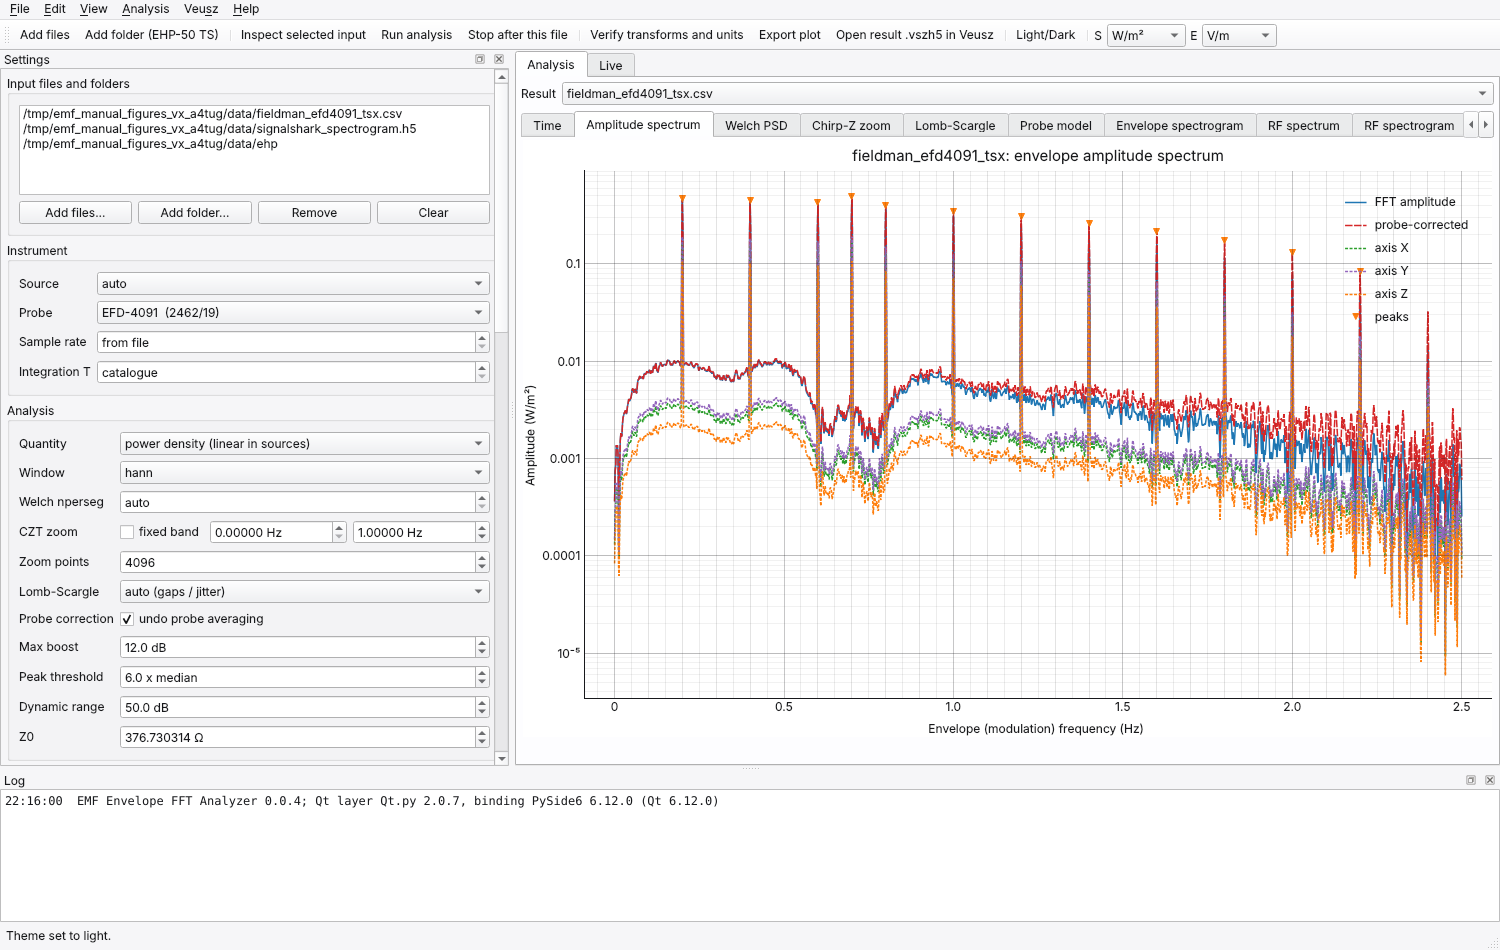
\includegraphics[width=0.92\linewidth]{figures/fig_gui_light.png}}{\fbox{\parbox{0.8\linewidth}{\centering Figure file \path{figures/fig_gui_light.png} not found: run \path{tools/build_manual_pdf.py --figures}.}}}
\caption{Main window, light theme: settings dock (left), toolbar, result selector and tabs (amplitude spectrum of a FieldMan/EFD-4091 log with the probe-corrected trace, X/Y/Z axes and peak markers), log dock and status bar. \emph{(Synthetic data.)}}\label{fig:gui_light}
\end{figure}


\begingroup\footnotesize
\begin{longtable}{@{}L{\dimexpr 0.17\linewidth-2\tabcolsep\relax}L{\dimexpr 0.45\linewidth-2\tabcolsep\relax}L{\dimexpr 0.34\linewidth-2\tabcolsep\relax}@{}}
\caption{Settings panel groups and the matching command-line options.}\label{tab:gui_settings}\\
\toprule
\textbf{Group} & \textbf{Fields} & \textbf{Command line} \\
\midrule
\endfirsthead
\multicolumn{3}{@{}l}{\itshape\footnotesize Table \thetable{} (continued)}\\
\toprule
\textbf{Group} & \textbf{Fields} & \textbf{Command line} \\
\midrule
\endhead
\bottomrule
\endlastfoot
Input files & list, Add files, Add folder, Remove, Clear; drag and drop; right-click menu & positional inputs \\
Instrument & Source, Probe, Sample rate, Integration T & -\kern0pt-source, -\kern0pt-probe, -\kern0pt-fs, -\kern0pt-t-int \\
Analysis & Quantity, Window, Welch nperseg, CZT zoom band and points, Lomb-Scargle, Probe correction, Max boost, Peak threshold, Dynamic range, Z0 & -\kern0pt-quantity, -\kern0pt-window, -\kern0pt-nperseg, -\kern0pt-zoom, -\kern0pt-zoom-points, -\kern0pt-lomb, -\kern0pt-correct-probe, -\kern0pt-max-boost-db, -\kern0pt-snr, -\kern0pt-dyn-range-db, -\kern0pt-z0 \\
Spectrograms & Channels, antenna factor, RBW, ENBW factor & -\kern0pt-rf-channels, -\kern0pt-antenna-factor-db, -\kern0pt-rbw-hz, -\kern0pt-enbw-factor \\
Columns and format & Time column, Value column, Unit, Delimiter, Decimal mark, Day first, HDF5 levels/frequency/time & -\kern0pt-time-col, -\kern0pt-value-col, -\kern0pt-unit, -\kern0pt-sep, -\kern0pt-decimal, -\kern0pt-dayfirst, -\kern0pt-h5-level/-\kern0pt-h5-freq/-\kern0pt-h5-time \\
Output & write files, folder, render with Veusz, pickle, parallel files, GPU & -\kern0pt-out, -\kern0pt-render, -\kern0pt-pickle, -\kern0pt-jobs, -\kern0pt-gpu \\
Units and display & one unit per family (power density, E, H, B, port power, port voltage), Time plot shows, RF levels as, Spectrum y axis (re-plot at once) & -\kern0pt-display-unit LIST, -\kern0pt-time-display, -\kern0pt-rf-level-display \\
Veusz documents in several units & tick list of every unit, layout (sections or files) & -\kern0pt-veusz-units LIST, -\kern0pt-veusz-layout \\
\end{longtable}
\endgroup


\begingroup\footnotesize
\begin{longtable}{@{}L{\dimexpr 0.22\linewidth-2\tabcolsep\relax}L{\dimexpr 0.74\linewidth-2\tabcolsep\relax}@{}}
\caption{Result tabs of the Analysis tab.}\label{tab:gui_tabs}\\
\toprule
\textbf{Tab} & \textbf{Shows} \\
\midrule
\endfirsthead
\multicolumn{2}{@{}l}{\itshape\footnotesize Table \thetable{} (continued)}\\
\toprule
\textbf{Tab} & \textbf{Shows} \\
\midrule
\endhead
\bottomrule
\endlastfoot
Time & power density, E or H (plane wave), the logged field or the analysed quantity, in the chosen units; date axis when the instrument clock is known \\
Amplitude spectrum & FFT amplitude (log, linear or dB), probe-corrected, X/Y/Z axes, peak markers \\
Welch PSD & PSD in dB re 1 (display unit)\textasciicircum{}2/Hz \\
Chirp-Z zoom & dense CZT samples and the FFT bins around the strongest line \\
Lomb-Scargle & amplitude from the raw time stamps against the FFT \\
Probe model & 20 log10 |sinc(f T)| \\
Envelope spectrogram & short-time PSD, time x envelope frequency \\
RF spectrum, RF spectrogram & mean/max-hold spectrum and level image of a spectrogram input in the power-density unit or as plane-wave E or H (RF levels as) \\
Modulation map & envelope spectrum of every frequency bin (dB rel. max) \\
Peaks and families & peak table (frequency, amplitude, SNR, CZT values, period) and harmonic families with rpm \\
Summary & readable summary, files written, and the summary file content (SI) \\
Inspect & how the selected inputs are read \\
Verification & the verify\_transforms table (Analysis > Verify) \\
\end{longtable}
\endgroup


\subsection{Units, display and themes}\label{sec:gui_units}
The \emph{Units and display} group of the settings panel (Figure~\ref{fig:gui_units})
holds one unit selector per quantity family: power density, electric field $E$,
magnetic field $H$, magnetic flux density $B$, port power and port voltage
(the last two for dBm or dB\textmu V levels without an antenna factor); the
same choices are in \emph{View $\rightarrow$ Units}, and the power-density and
E-field units are also on the toolbar. Each family offers linear units and
level (dB) units, 34 in all (Table~\ref{tab:units},
Section~\ref{sec:units}): a result is shown in the unit chosen for the family of
its analysed quantity, so a FieldMan log in mW/cm$^2$ and a SignalShark channel
in dBm at the port can be on screen with their own units at the same time.
\emph{Time plot shows} selects the power density, $E$ or $H$ of the equivalent
plane wave, the logged field, or the analysed quantity (Table~\ref{tab:modes});
when the choice cannot be derived from a record (for example $E$ of a dBm port
log) the analysed quantity is shown and the axis says so. \emph{RF levels as}
shows the spectrum and spectrogram levels of power-density inputs as power
density or as plane-wave $E$ or $H$. \emph{Spectrum y axis} selects a
logarithmic, linear or dB-relative (20\,log10) amplitude axis; level units are
always drawn on a linear axis. Every change re-plots at once without
re-analysing: results are kept in SI units, and the peaks table, the summary
and the live plots follow the same choices.

The \emph{Veusz documents in several units} group lists every unit with a tick
box; the ticked units are added to the Veusz output besides the display units,
either as sections of one document or as one document per unit
(Section~\ref{sec:multiunit}). \emph{Veusz $\rightarrow$ Write .vszh5 again}
(Ctrl+Shift+W) re-writes the selected result's document(s) in the current units
without analysing again, and renders them when \emph{Render} is ticked.

\emph{View $\rightarrow$ Theme} selects System default, Light or Dark
(Figure~\ref{fig:gui_dark}); the theme recolours the window and every plot, and
is remembered.

\begin{figure}[htbp]
\centering
\IfFileExists{figures/fig_gui_units.png}{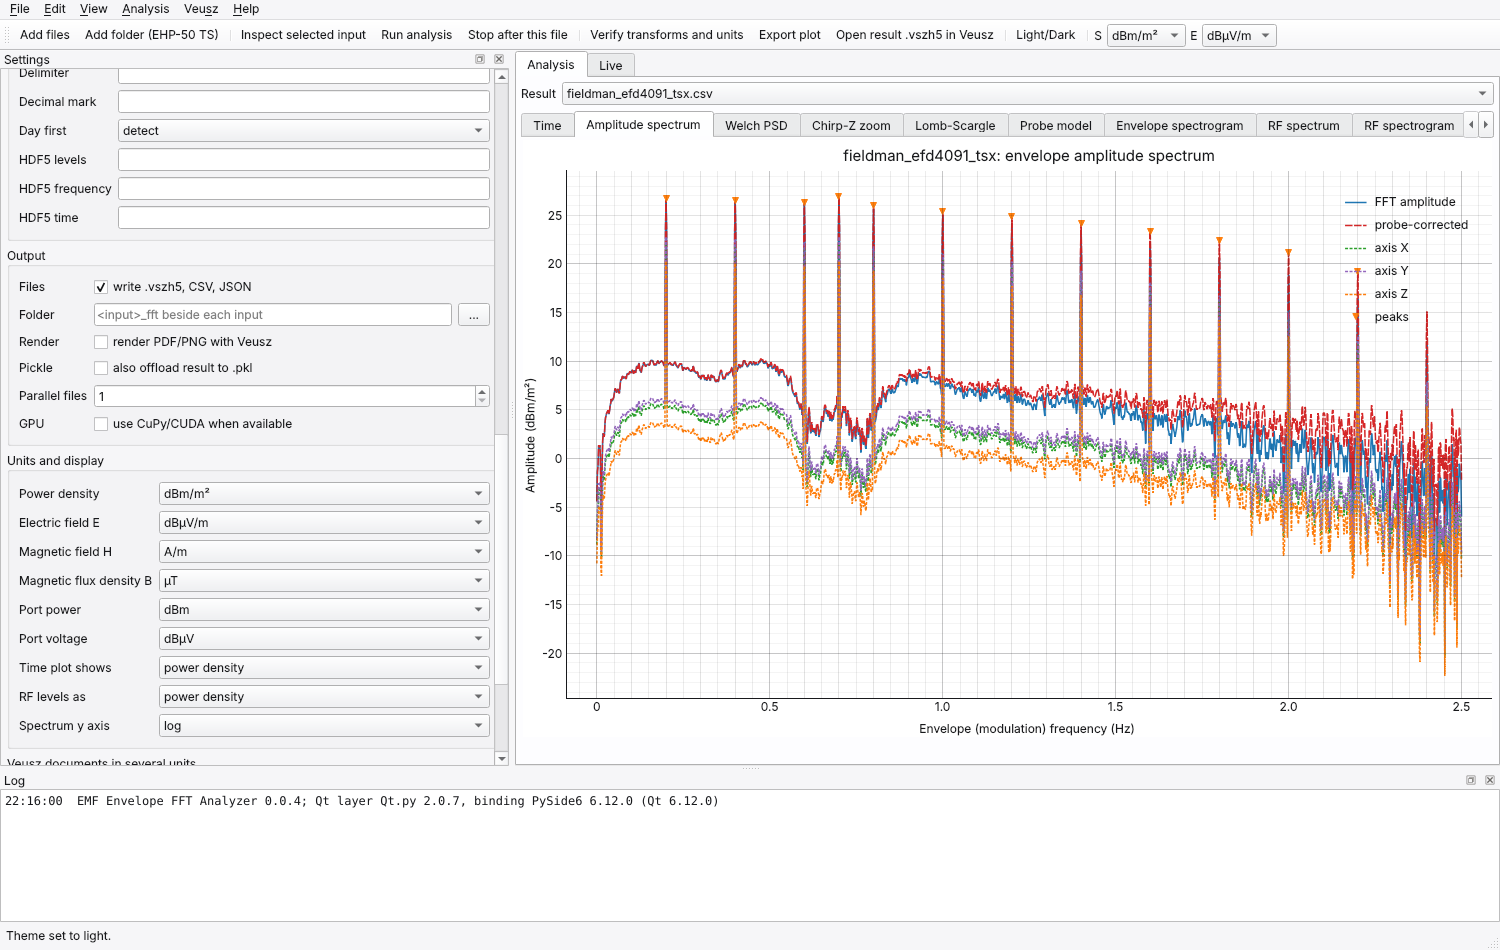
\includegraphics[width=0.92\linewidth]{figures/fig_gui_units.png}}{\fbox{\parbox{0.8\linewidth}{\centering Figure file \path{figures/fig_gui_units.png} not found: run \path{tools/build_manual_pdf.py --figures}.}}}
\caption{Units and display group (left, scrolled into view): one unit per quantity family, time-plot and RF-level modes; the amplitude spectrum in dBm/m$^2$ (a level unit, so a linear axis) and the toolbar S and E unit selectors. \emph{(Synthetic data.)}}\label{fig:gui_units}
\end{figure}


\begin{figure}[htbp]
\centering
\IfFileExists{figures/fig_gui_dark.png}{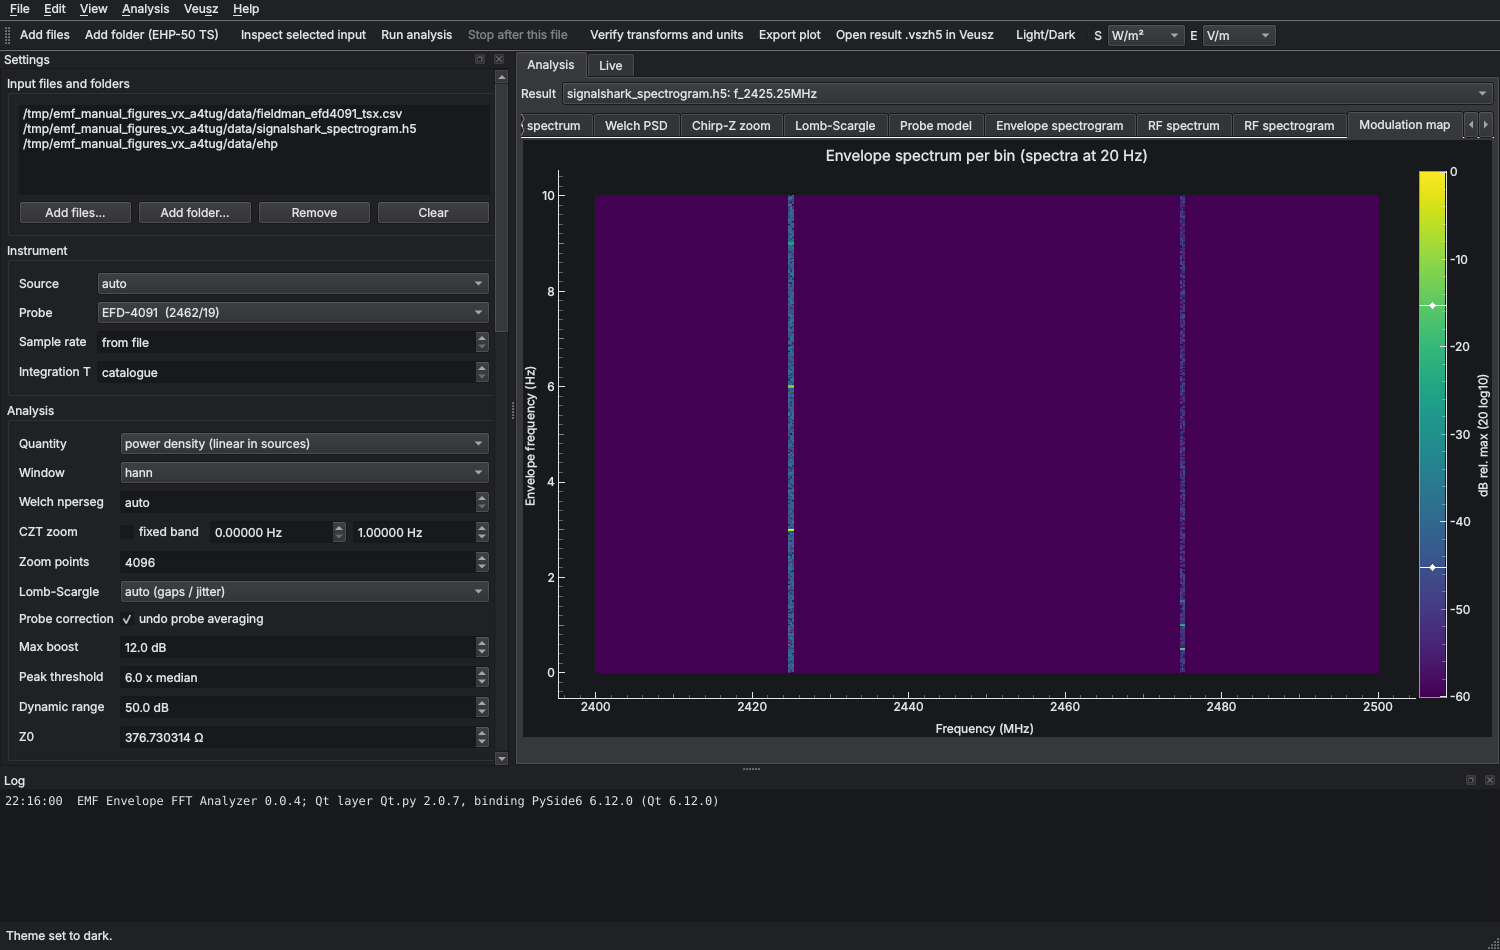
\includegraphics[width=0.92\linewidth]{figures/fig_gui_dark.png}}{\fbox{\parbox{0.8\linewidth}{\centering Figure file \path{figures/fig_gui_dark.png} not found: run \path{tools/build_manual_pdf.py --figures}.}}}
\caption{Dark theme: modulation map of a SignalShark spectrogram channel. \emph{(Synthetic data.)}}\label{fig:gui_dark}
\end{figure}


\subsection{Menus and keyboard shortcuts}
Table~\ref{tab:gui_menus} lists every menu command, read from the running window
when this manual was built; \emph{Help $\rightarrow$ Keyboard shortcuts} shows the
shortcuts and \emph{Help $\rightarrow$ Probe catalogue} the probe table with its
derived limits. Settings, window layout, theme, last folder and the recent inputs
are kept between sessions (QSettings); \emph{File $\rightarrow$ Save settings} and
\emph{Load settings} store and restore the options as JSON, and \emph{Reset
settings to defaults} restores the defaults.

\begingroup\footnotesize
\begin{longtable}{@{}L{\dimexpr 0.3\linewidth-2\tabcolsep\relax}L{\dimexpr 0.48\linewidth-2\tabcolsep\relax}L{\dimexpr 0.18\linewidth-2\tabcolsep\relax}@{}}
\caption{Menu commands of the main window (read from the running window).}\label{tab:gui_menus}\\
\toprule
\textbf{Menu} & \textbf{Command} & \textbf{Shortcut} \\
\midrule
\endfirsthead
\multicolumn{3}{@{}l}{\itshape\footnotesize Table \thetable{} (continued)}\\
\toprule
\textbf{Menu} & \textbf{Command} & \textbf{Shortcut} \\
\midrule
\endhead
\bottomrule
\endlastfoot
File & Add files... & \texttt{Ctrl+O} \\
File & Add folder (EHP-50 TS)... & \texttt{Ctrl+Shift+O} \\
File & Clear inputs &  \\
File & Export current plot (PNG, SVG, CSV)... & \texttt{Ctrl+E} \\
File & Export peaks table (CSV)... &  \\
File & Save log... &  \\
File & Open output folder &  \\
File & Load settings... &  \\
File & Save settings... & \texttt{Ctrl+S} \\
File & Reset settings to defaults &  \\
File & Quit &  \\
Edit & Copy summary & \texttt{Ctrl+Shift+S} \\
Edit & Copy peaks table & \texttt{Ctrl+Shift+P} \\
Edit & Copy log &  \\
Edit & Clear log &  \\
Edit & Clear results &  \\
Edit & Free memory (results, live buffer, GC) &  \\
View > Theme & System default &  \\
View > Theme & Light &  \\
View > Theme & Dark &  \\
View > Units > Power density & one of: W/m², mW/m², µW/m², mW/cm², µW/cm², nW/cm², dBW/m², dBm/m² &  \\
View > Units > Electric field E & one of: V/m, mV/m, µV/m, kV/m, dBV/m, dBµV/m &  \\
View > Units > Magnetic field H & one of: A/m, mA/m, µA/m, dBµA/m &  \\
View > Units > Magnetic flux density B & one of: T, mT, µT, nT, pT &  \\
View > Units > Port power & one of: W, mW, µW, nW, dBW, dBm &  \\
View > Units > Port voltage & one of: V, mV, µV, dBV, dBµV &  \\
View > Time plot shows & one of: power density, E field, H field, logged field, analysed quantity &  \\
View > RF levels as & power density &  \\
View > RF levels as & E field &  \\
View > RF levels as & H field &  \\
View > Spectrum y axis & log &  \\
View > Spectrum y axis & linear &  \\
View > Spectrum y axis & dB rel. max (20 log10) &  \\
View & Auto-range current plot & \texttt{Ctrl+0} \\
View & Toolbar &  \\
View & Settings panel & \texttt{Ctrl+Shift+E} \\
View & Log panel & \texttt{Ctrl+Shift+L} \\
View & Full screen & \texttt{F11} \\
Analysis & Inspect selected input & \texttt{Ctrl+I} \\
Analysis & Run analysis & \texttt{F5} \\
Analysis & Stop after this file & \texttt{Esc} \\
Analysis & Verify transforms and units & \texttt{Ctrl+Shift+V} \\
Analysis & Run self-test &  \\
Analysis & Live mode & \texttt{Ctrl+L} \\
Veusz & Open result .vszh5 in Veusz & \texttt{Ctrl+Shift+Z} \\
Veusz & Write .vszh5 again (current units) & \texttt{Ctrl+Shift+W} \\
Veusz & Render result to PDF/PNG &  \\
Veusz & Open rendered PDF &  \\
Help & User manual (PDF) & \texttt{F1} \\
Help & Keyboard shortcuts &  \\
Help & Probe catalogue &  \\
Help & About EMF Envelope FFT Analyzer &  \\
Help & About Qt &  \\
\end{longtable}
\endgroup


\subsection{About dialog}
\emph{Help $\rightarrow$ About} (Figure~\ref{fig:gui_about}) shows the program name
and version, the author, company and e-mail address, the licence (GNU General
Public License v3.0 or later) with its warranty notice and a link to the licence
text, and under \emph{Show Details} the versions of Python, the Qt layer and
binding, pyqtgraph, NumPy, SciPy, pandas, h5py and the Veusz writer.

\begin{figure}[htbp]
\centering
\IfFileExists{figures/fig_gui_about.png}{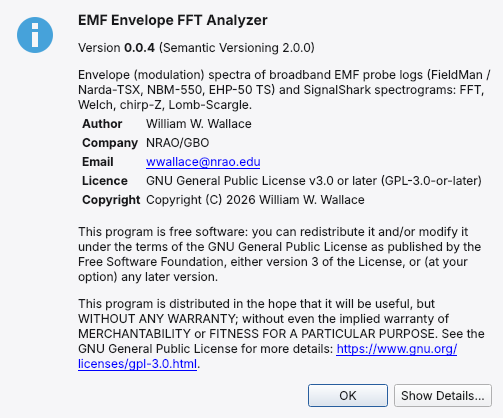
\includegraphics[width=0.92\linewidth]{figures/fig_gui_about.png}}{\fbox{\parbox{0.8\linewidth}{\centering Figure file \path{figures/fig_gui_about.png} not found: run \path{tools/build_manual_pdf.py --figures}.}}}
\caption{Help $\rightarrow$ About: author, version and the GPL-3.0-or-later licence. \emph{(Synthetic data.)}}\label{fig:gui_about}
\end{figure}


% =============================================================================
%    4  INSTRUMENTS AND INPUT FILES
% =============================================================================
\section{Instruments and input files}\label{sec:inputs}

\subsection{Probe catalogue}
Table~\ref{tab:probes} lists the probes the program knows, from the
datasheets. \texttt{--probe} accepts the names in the first column (case and
spaces ignored) and the aliases \texttt{EFD-4091E} (treated as the EFD-4091;
no separate datasheet for an ``E'' variant was found), \texttt{EF-0691},
\texttt{EFD-1891FAST} and the forms without hyphens. The last four columns are
derived: the Nyquist frequency $f_s/2$, the response of the probe's averaging at
that frequency, and the first null $1/T$ of that response
(Section~\ref{sec:sinc}).

\begingroup\footnotesize
\begin{longtable}{@{}L{\dimexpr 0.14\linewidth-2\tabcolsep\relax}L{\dimexpr 0.13\linewidth-2\tabcolsep\relax}L{\dimexpr 0.07\linewidth-2\tabcolsep\relax}L{\dimexpr 0.1\linewidth-2\tabcolsep\relax}L{\dimexpr 0.08\linewidth-2\tabcolsep\relax}L{\dimexpr 0.1\linewidth-2\tabcolsep\relax}L{\dimexpr 0.08\linewidth-2\tabcolsep\relax}L{\dimexpr 0.1\linewidth-2\tabcolsep\relax}L{\dimexpr 0.08\linewidth-2\tabcolsep\relax}L{\dimexpr 0.08\linewidth-2\tabcolsep\relax}@{}}
\caption{Probe catalogue (datasheet values) and the derived envelope limits.}\label{tab:probes}\\
\toprule
\textbf{Probe} & \textbf{RF range} & \textbf{$f_s$ (Hz)} & \textbf{$T$ (ms)} & \textbf{$\nu_N$ (Hz)} & \textbf{$|H(\nu_N)|$ (dB)} & \textbf{$1/T$ (Hz)} & \textbf{True RMS to (V/m)} & \textbf{Axes} & \textbf{Ref.} \\
\midrule
\endfirsthead
\multicolumn{10}{@{}l}{\itshape\footnotesize Table \thetable{} (continued)}\\
\toprule
\textbf{Probe} & \textbf{RF range} & \textbf{$f_s$ (Hz)} & \textbf{$T$ (ms)} & \textbf{$\nu_N$ (Hz)} & \textbf{$|H(\nu_N)|$ (dB)} & \textbf{$1/T$ (Hz)} & \textbf{True RMS to (V/m)} & \textbf{Axes} & \textbf{Ref.} \\
\midrule
\endhead
\bottomrule
\endlastfoot
EFD-4091\newline\footnotesize 2462/19 & 2 MHz -\kern0pt- 40 GHz & 5 & 265 & 2.5 & -7.6 & 3.774 & 65 & rss & \cite{R1} \\
EFD-0691\newline\footnotesize 2462/14B & 100 kHz -\kern0pt- 6 GHz & 5 & 265 & 2.5 & -7.6 & 3.774 & 17 & xyz & \cite{R2} \\
EF 0691 (NBM)\newline\footnotesize NBM probe & 100 kHz -\kern0pt- 6 GHz & 5 & n/p\newline\footnotesize(1/fs used) & 2.5 & -3.9 & 5 & 22 & rss & \cite{R6} \\
EFD-9091\newline\footnotesize 2462/18 & 100 MHz -\kern0pt- 90 GHz & 5 & 275 & 2.5 & -8.3 & 3.636 & 61.4 & rss & \cite{R3} \\
EFD-1891 Fast\newline\footnotesize 2462/23 & 2 MHz -\kern0pt- 18 GHz & 900 & 2.3 & 450 & -29.4 & 434.8 & -- & rss & \cite{R4} \\
\end{longtable}
\endgroup


\subsection{Readers}
The reader is chosen from the file (Table~\ref{tab:readers}); \texttt{--source}
forces one.

\begingroup\small
\begin{longtable}{@{}L{\dimexpr 0.14\linewidth-2\tabcolsep\relax}L{\dimexpr 0.22\linewidth-2\tabcolsep\relax}L{\dimexpr 0.16\linewidth-2\tabcolsep\relax}L{\dimexpr 0.24\linewidth-2\tabcolsep\relax}L{\dimexpr 0.2\linewidth-2\tabcolsep\relax}@{}}
\caption{Readers and how the input is recognised.}\label{tab:readers}\\
\toprule
\textbf{\texttt{--source}} & \textbf{Instrument / software} & \textbf{Files} & \textbf{Auto-detected when} & \textbf{Result} \\
\midrule
\endfirsthead
\multicolumn{5}{@{}l}{\itshape\footnotesize Table \thetable{} (continued)}\\
\toprule
\textbf{\texttt{--source}} & \textbf{Instrument / software} & \textbf{Files} & \textbf{Auto-detected when} & \textbf{Result} \\
\midrule
\endhead
\bottomrule
\endlastfoot
\texttt{fieldman, tsx} & FieldMan or Narda-TSX with EFD-4091, -0691, -9091, -1891 & .csv .txt & default for text files & time series (+ X/Y/Z) \\
\texttt{nbm} & NBM-550 / NBM-TS with EF 0691 & .csv .txt & a column named 'Result ...' & time series \\
\texttt{xlsx} & any of the above saved as Excel & .xlsx .xls & by extension & time series \\
\texttt{ehp} & EHP-50 TS with EHP-50F (1 Hz - 400 kHz) & folder, \path{hh_mm_ss_cc.TXT} & a folder, or the EHP file name & spectrogram (folder), spectrum, or time series (logger file) \\
\texttt{signalshark} & SignalShark & .h5 .hdf5; converter .csv & .h5 extension; 8+ numeric column names or a frequency column & spectrogram (or level time series) \\
\end{longtable}
\endgroup


\subsection{How text exports are read}\label{sec:textreading}
Narda's software is German-made, so semicolon-separated files with a decimal
comma are expected as often as comma-separated files with a decimal point.
\begin{enumerate}
\item \textbf{Encoding}: UTF-8 (with or without byte-order mark), then
Windows-1252, then Latin-1.
\item \textbf{Delimiter}: the first of tab, \texttt{;}, \texttt{,}, \texttt{|}
that occurs the same number of times on the last 50 non-blank lines;
whitespace otherwise. Semicolon is tried before comma because a decimal comma
puts a comma inside every number.
\item \textbf{Decimal mark}: comma when numbers such as \texttt{1,23} appear
and the delimiter is not a comma.
\item \textbf{Header row}: the first row with the same number of fields as the
row below it and more text fields than that row, whose fields are mostly
numbers or date/times. Lines above it are kept as metadata and searched for a
unit.
\item \textbf{Columns}: chosen with the keyword lists of Table~\ref{tab:keywords};
the unit comes from \texttt{--unit}, the value column's header or the
metadata, in that order.
\item \textbf{Time}: numbers are seconds (milliseconds when the header says
\texttt{ms}); anything else is parsed as date/time, day first when dates look
like \texttt{dd.mm.yyyy}. A date column and a clock column are joined. The
first value is the origin of every chunk of a large file, so the time axis is
continuous.
\item \textbf{Size}: the file is read in chunks of 500\,000 rows; columns longer
than 20\,000\,000 samples move to a temporary file on disk (Section~\ref{sec:memory}).
\end{enumerate}

\begingroup\footnotesize
\begin{longtable}{@{}L{\dimexpr 0.2\linewidth-2\tabcolsep\relax}L{\dimexpr 0.46\linewidth-2\tabcolsep\relax}L{\dimexpr 0.3\linewidth-2\tabcolsep\relax}@{}}
\caption{Keywords that select columns (case ignored).}\label{tab:keywords}\\
\toprule
\textbf{Use} & \textbf{Keywords} & \textbf{Note} \\
\midrule
\endfirsthead
\multicolumn{3}{@{}l}{\itshape\footnotesize Table \thetable{} (continued)}\\
\toprule
\textbf{Use} & \textbf{Keywords} & \textbf{Note} \\
\midrule
\endhead
\bottomrule
\endlastfoot
time column & \texttt{time}, \texttt{zeit}, \texttt{uhrzeit}, \texttt{timestamp}, \texttt{date}, \texttt{datum}, \texttt{elapsed}, \texttt{t [s]}, \texttt{t(s)}, \texttt{t/s}, \texttt{sec}, \texttt{hh:mm} & a date column and a clock column are joined; otherwise the first match \\
value column, preferred (+5) & \texttt{actual}, \texttt{act}, \texttt{rss}, \texttt{total}, \texttt{result 1}, \texttt{isotrop}, \texttt{value}, \texttt{wert}, \texttt{e-field}, \texttt{e field}, \texttt{field}, \texttt{level} & +3 more if the header names a unit; leftmost column wins ties \\
value column, avoided (-6) & \texttt{max}, \texttt{min}, \texttt{avg}, \texttt{mean}, \texttt{average}, \texttt{batt}, \texttt{temp}, \texttt{humid}, \texttt{press}, \texttt{lat}, \texttt{lon}, \texttt{alt}, \texttt{gps}, \texttt{index}, \texttt{no.}, \texttt{nr}, \texttt{flag}, \texttt{dist}, \texttt{comment} & statistics and house-keeping columns \\
axis columns & \texttt{X, Y, Z, E\_x, H y, field\_z, ...} & used for per-axis spectra; their RSS is the value when no value column exists \\
\end{longtable}
\endgroup


\subsection{EHP-50 TS spectra}
EHP-50 TS saves one spectrum per file as \path{YYYY/MM/DD/hh_mm_ss_cc.TXT}
($cc$ = hundredths of a second) \cite{R7}. Given a folder, the program reads
every \texttt{.txt}/\texttt{.csv} below it, takes the time of each spectrum from
its path (the file date when the name does not match), sorts them, and puts
every spectrum on the frequency axis of the first one (linear interpolation
when they differ). The total or RSS column is preferred over X, Y, Z. The result
is analysed as a spectrogram (Section~\ref{sec:spectrogram}). Note that EHP-50 TS
records only the EHP-50F (1\,Hz to 400\,kHz); it cannot record the RF probes.

\subsection{SignalShark files}
The layout of SignalShark's \texttt{.h5} files is not published. The reader
takes the largest two-dimensional numeric dataset as levels (time $\times$
frequency, transposed if the axes say so), a one-dimensional dataset of matching
length whose name or values look like frequencies as the frequency axis, and one
that increases as the time axis; otherwise start/stop/centre/span and
time-resolution attributes. \texttt{--h5-level}, \texttt{--h5-freq} and
\texttt{--h5-time} name the datasets explicitly; \texttt{--inspect} prints the
whole HDF5 tree. CSV files made with Narda's NSL \emph{Converter} script
\cite{R8} are read in wide format (one row per spectrum, the header holding the
frequencies), long format (time, frequency, level columns) or transposed wide
format (one row per frequency). Levels in dBm or dB\textmu V are converted to
field strength only when an antenna factor is given (\texttt{--antenna-factor-db}).

\subsection{Overriding the detection}\label{sec:overrides}
\texttt{--source}, \texttt{--time-col} (\texttt{"Date+Time"} joins two columns),
\texttt{--value-col}, \texttt{--unit}, \texttt{--sep}, \texttt{--decimal},
\texttt{--dayfirst} and \texttt{--fs} (for files without a time column) override
the corresponding guess. Column names or zero-based indices are accepted.

% =============================================================================
%    6  METHODS: THEORY AND IMPLEMENTATION
% =============================================================================
\section{Methods: theory and implementation}\label{sec:theory}

This section describes every method the program uses: the physics of the
measurement, the unit conversions, and each time-to-frequency transform
(FFT amplitude spectrum, Welch power spectral density, chirp-Z zoom,
Lomb--Scargle periodogram, short-time FFT), followed by the probe model,
peak finding, harmonic families and the spectrogram methods. For each
transform it gives the idea, the derivation, the algorithm as implemented,
the parameters and their trade-offs, and how its correctness was verified
(Section~\ref{sec:verification}). Table~\ref{tab:methods} is an overview.

\begingroup\footnotesize
\begin{longtable}{@{}L{\dimexpr 0.16\linewidth-2\tabcolsep\relax}L{\dimexpr 0.26\linewidth-2\tabcolsep\relax}L{\dimexpr 0.2\linewidth-2\tabcolsep\relax}L{\dimexpr 0.16\linewidth-2\tabcolsep\relax}L{\dimexpr 0.18\linewidth-2\tabcolsep\relax}@{}}
\caption{The methods at a glance.}\label{tab:methods}\\
\toprule
\textbf{Method} & \textbf{Question it answers} & \textbf{Output (unit)} & \textbf{Resolution} & \textbf{Used} \\
\midrule
\endfirsthead
\multicolumn{5}{@{}l}{\itshape\footnotesize Table \thetable{} (continued)}\\
\toprule
\textbf{Method} & \textbf{Question it answers} & \textbf{Output (unit)} & \textbf{Resolution} & \textbf{Used} \\
\midrule
\endhead
\bottomrule
\endlastfoot
FFT amplitude & how strong is each modulation frequency? & amplitude (W/m2) & fs/N & always \\
Welch PSD & how is envelope power spread? noise floor & PSD ((W/m2)\textasciicircum{}2/Hz) & ENBW fs/L & always \\
Chirp-Z zoom & exact frequency and amplitude of a line & amplitude (W/m2) & fs/N (dense samples) & around the strongest line, or -\kern0pt-zoom \\
Lomb-Scargle & spectrum without resampling irregular stamps & amplitude (W/m2) & 1/T\_span & gaps or jitter, or -\kern0pt-lomb on \\
Short-time FFT & does a modulation come and go? & PSD vs time & fs/L and L/fs & long logs \\
Probe model & how much does the probe's averaging attenuate? & |H| (20 log10) & -- & probe or T known \\
Per-bin modulation & which RF carrier is modulated at which rate? & dB rel. max & spectra rate / N\_t & spectrograms \\
\end{longtable}
\endgroup


\subsection{Square-law detection adds powers}\label{sec:powersum}
A diode detector operated in its square-law region delivers a voltage
proportional to the square of the RF voltage. Let the field at the probe be the
sum of $M$ sources,
\begin{equation}
E(t) = \sum_{i=1}^{M} E_i \cos(2\pi f_i t + \varphi_i).
\end{equation}
The detector output, averaged by a video filter that is much slower than any
difference frequency $|f_i - f_j|$, is
\begin{align}
\overline{E^2} &= \sum_{i}\sum_{j} E_i E_j\,\overline{\cos(2\pi f_i t+\varphi_i)\cos(2\pi f_j t+\varphi_j)} \nonumber\\
&= \sum_{i}\sum_{j} \frac{E_i E_j}{2}\Big[\overline{\cos\big(2\pi(f_i-f_j)t+\varphi_i-\varphi_j\big)}
 + \overline{\cos\big(2\pi(f_i+f_j)t+\varphi_i+\varphi_j\big)}\Big] \nonumber\\
&= \sum_{i} \frac{E_i^2}{2} = \sum_i E_{i,\mathrm{rms}}^2,
\label{eq:powersum}
\end{align}
because every term with $i\neq j$ and every sum-frequency term averages to
zero. Three orthogonal sensors add in the same way,
$E^2 = E_x^2 + E_y^2 + E_z^2$ (the isotropic RSS value). With the probe's
frequency response $r(f)$ and the plane-wave power density
$S = E_\mathrm{rms}^2 / Z_0$, the displayed value is
\begin{equation}
S_\mathrm{disp}(t) = \sum_i r(f_i)\, S_i(t),\qquad
E_\mathrm{disp}(t) = \sqrt{Z_0\, S_\mathrm{disp}(t)}.
\label{eq:sdisp}
\end{equation}
Equation~\eqref{eq:powersum} holds only while every diode stays in its
square-law region, which for the EFD probes is the True-RMS range of
Table~\ref{tab:probes}; above it the program warns.

\subsection{Why the transform is taken of power}\label{sec:whypower}
The Fourier transform is linear, so applying it to \eqref{eq:sdisp} gives
\begin{equation}
\mathcal{F}\{S_\mathrm{disp}\}(\nu) = \sum_i r(f_i)\,\mathcal{F}\{S_i\}(\nu):
\label{eq:linear}
\end{equation}
the envelope spectrum of the log is the weighted sum of the envelope spectra of
the sources, and each source's modulation lines appear unchanged. The field
$E_\mathrm{disp} = \sqrt{Z_0 S_\mathrm{disp}}$ does not have this property. Take
two sources $S_1 = a + b\cos 2\pi\nu_1 t$ and $S_2 = c + d\cos 2\pi\nu_2 t$ with
$A = a+c$ and $x(t) = b\cos 2\pi\nu_1 t + d\cos 2\pi\nu_2 t$, $|x| < A$. The
Taylor series of the square root gives
\begin{align}
\sqrt{A + x} &= \sqrt{A}\left(1 + \frac{x}{2A} - \frac{x^2}{8A^2} + \dots\right),\\
x^2 &= \frac{b^2+d^2}{2} + \frac{b^2}{2}\cos 4\pi\nu_1 t + \frac{d^2}{2}\cos 4\pi\nu_2 t \nonumber\\
 &\quad + bd\,\big[\cos 2\pi(\nu_1-\nu_2)t + \cos 2\pi(\nu_1+\nu_2)t\big],
\end{align}
so the spectrum of $E$ contains lines at $2\nu_1$, $2\nu_2$ and
$\nu_1\pm\nu_2$ that no source produces (intermodulation). The program
therefore analyses power density (W/m$^2$) by default (\texttt{--quantity power});
\texttt{field} and \texttt{db} are available for comparison only.

\subsection{Units, conversions and dB conventions}\label{sec:units}
\paragraph{Electric and magnetic field.}
For a plane wave in free space the Poynting vector has the magnitude
$S = E\,H$ and the fields are in the ratio $E/H = Z_0 = \mu_0 c$, so
\begin{equation}
S = E H = \frac{E^2}{Z_0} = Z_0 H^2,\qquad E = \sqrt{S Z_0},\qquad H = \sqrt{S/Z_0}.
\label{eq:planewave}
\end{equation}
The program uses $Z_0 = 376.730313668\,\Omega$ (from the CODATA~2018 $\mu_0$); the
CODATA~2022 value is $376.730\,313\,412(59)\,\Omega$ \cite{B32}, a difference of
$7\times10^{-10}$. Narda's displays use round conversions near 377\,$\Omega$;
\texttt{--z0 377} reproduces them. Readings of $E$, $H$ or a power density are
converted to $S$ in W/m$^2$ for the analysis; magnetic flux density is analysed
as $B^2$ (proportional to the magnetic energy density), and EHP-50F fields as
the field squared, because at 1\,Hz--400\,kHz the fields are quasi-static and no
plane-wave power density exists. Equation~(\ref{eq:planewave}) holds only in the
far field; the conversions of the time plots below rely on it.

\begingroup\footnotesize
\begin{longtable}{@{}L{\dimexpr 0.2\linewidth-2\tabcolsep\relax}L{\dimexpr 0.3\linewidth-2\tabcolsep\relax}L{\dimexpr 0.3\linewidth-2\tabcolsep\relax}@{}}
\caption{Power-density input units: W/m$^2$ per unit (reading $\times$ factor $=$ W/m$^2$).}\label{tab:input_units}\\
\toprule
\textbf{Key} & \textbf{W/m$^2$ per unit} & \textbf{Label} \\
\midrule
\endfirsthead
\multicolumn{3}{@{}l}{\itshape\footnotesize Table \thetable{} (continued)}\\
\toprule
\textbf{Key} & \textbf{W/m$^2$ per unit} & \textbf{Label} \\
\midrule
\endhead
\bottomrule
\endlastfoot
\texttt{W/m2} & 1 & W/m² \\
\texttt{mW/m2} & 0.001 & mW/m² \\
\texttt{uW/m2} & 1e-06 & µW/m² \\
\texttt{mW/cm2} & 10 & mW/cm² \\
\texttt{uW/cm2} & 0.01 & µW/cm² \\
\texttt{nW/cm2} & 1e-05 & nW/cm² \\
\end{longtable}
\endgroup


\paragraph{Logarithmic input units.}
From dB\textmu V/m: $E = 10^{(L-120)/20}$\,V/m, because
$L = 20\log_{10}(E/1\,\mathrm{\upmu V/m})$ and $1\,\mathrm{\upmu V} = 10^{-6}\,\mathrm{V}$.
From dBm at a 50\,$\Omega$ port, $P = V^2/R$ gives
\begin{align}
L_{\mathrm{dB\upmu V}} &= 20\log_{10}\frac{V}{1\,\mathrm{\upmu V}}
 = 10\log_{10}\frac{P R}{10^{-12}\,\mathrm{V^2}} \nonumber\\
 &= 10\log_{10}\frac{P}{1\,\mathrm{mW}} + 10\log_{10}\frac{10^{-3}\cdot 50}{10^{-12}}
 = L_\mathrm{dBm} + 106.9897,
\end{align}
which the program uses exactly (version 0.0.2 used the rounded 107\,dB). With
the antenna factor $\mathit{AF} = E/V$ in dB(1/m),
$L_{\mathrm{dB\upmu V/m}} = L_{\mathrm{dB\upmu V}} + \mathit{AF}$; without
\texttt{--antenna-factor-db}, dBm levels are analysed as mW at the analyzer port
and dB\textmu V levels as \textmu V$^2$. A power density in dBm/m$^2$ is
$10^{L/10}$\,mW/m$^2$.

\paragraph{Display units: families and the two rules.}
Every analysed quantity belongs to a \emph{family} (Table~\ref{tab:quantity_families}):
power density (base unit W/m$^2$), electric field (V/m), magnetic field (A/m),
flux density (T), port power (mW) and port voltage (\textmu V). One display unit is
chosen per family (\texttt{--display-unit mW/cm2,dBuV/m}: each unit sets its own
family, the others keep their defaults). A value $x$ held in the family's base
unit is shown in a \emph{linear} unit as $k\,x$, where $k$ is the number of display
units per base unit (Table~\ref{tab:units}); for example
$1\,\mathrm{W/m^2} = 10^{-3}\,\mathrm{W}/10^{4}\,\mathrm{cm^2}\cdot 10^{3}\,\mathrm{mW/W}
= 0.1\,\mathrm{mW/cm^2}$, so $k = 0.1$. In a \emph{level} unit it is shown as
\begin{equation}
L = D\,\log_{10}(k\,x)\ \mathrm{dB},\qquad
D = \begin{cases}10 & \text{power quantities (power density, port power)},\\
20 & \text{root-power quantities (}E,\ H,\ \text{port voltage)},\end{cases}
\label{eq:level}
\end{equation}
the convention of IEC~60027-3 and ISO~80000-1 \cite{B41,B42}: the square of a
root-power quantity is proportional to power, so both give the same level
change for the same change of power. Hence $1\,\mathrm{W/m^2} = 0\,\mathrm{dBW/m^2}
= 30\,\mathrm{dBm/m^2}$ ($k = 10^3$), $1\,\mathrm{V/m} = 120\,\mathrm{dB\upmu V/m}$
($k=10^6$, $D=20$), $1\,\mathrm{mW} = 0\,\mathrm{dBm} = -30\,\mathrm{dBW}$. A
factor ten in $x$ changes $L$ by 10\,dB for power and 20\,dB for root-power
quantities. Values at or below zero have no level; they are clipped at
$10^{-15}$ of the largest value of the trace (NaN stays NaN).

\begingroup\footnotesize
\begin{longtable}{@{}L{\dimexpr 0.14\linewidth-2\tabcolsep\relax}L{\dimexpr 0.42\linewidth-2\tabcolsep\relax}L{\dimexpr 0.26\linewidth-2\tabcolsep\relax}L{\dimexpr 0.14\linewidth-2\tabcolsep\relax}@{}}
\caption{Analysed quantities, their origin and their unit family (\texttt{QUANTITY\_FAMILY}); the last column is the default display unit.}\label{tab:quantity_families}\\
\toprule
\textbf{Analysed} & \textbf{Comes from} & \textbf{Family} & \textbf{Default} \\
\midrule
\endfirsthead
\multicolumn{4}{@{}l}{\itshape\footnotesize Table \thetable{} (continued)}\\
\toprule
\textbf{Analysed} & \textbf{Comes from} & \textbf{Family} & \textbf{Default} \\
\midrule
\endhead
\bottomrule
\endlastfoot
\texttt{W/m\textasciicircum{}2} & power density: S logged, E\textasciicircum{}2/Z0, Z0 H\textasciicircum{}2, dBuV/m, or dBm/dBuV with an antenna factor & Power density & W/m² \\
\texttt{V/m} & E with -\kern0pt-quantity field (E logged or sqrt(S Z0)) & Electric field E & V/m \\
\texttt{A/m} & H with -\kern0pt-quantity field & Magnetic field H & A/m \\
\texttt{T} & B with -\kern0pt-quantity field & Magnetic flux density B & µT \\
\texttt{mW} & dBm at the analyzer port, no antenna factor & Port power (no antenna factor) & dBm \\
\texttt{uV\textasciicircum{}2} & dBuV at the analyzer port, no antenna factor & Port voltage (no antenna factor), squared & dB re 1 µV² \\
\texttt{T\textasciicircum{}2} & B logged, analysed as B\textasciicircum{}2 (power-like) & Magnetic flux density B, squared & µT² \\
\texttt{(V/m)\textasciicircum{}2} & EHP-50 TS E field squared (quasi-static, no Z0) & Electric field E, squared & (V/m)² \\
\texttt{(A/m)\textasciicircum{}2} & EHP-50 TS H field squared & Magnetic field H, squared & (A/m)² \\
\texttt{(T)\textasciicircum{}2} & EHP-50 TS B field squared & Magnetic flux density B, squared & µT² \\
\%, dB rel. max, a.u. & \% of standard, -\kern0pt-quantity db, unknown unit & none: shown as analysed & -- \\
\end{longtable}
\endgroup


\paragraph{Squared quantities.}
A field squared ($E^2$ of the EHP-50 TS, $B^2$, \textmu V$^2$) is shown in the
square of the unit chosen for its root family: with factor $k$ for the root,
$k^2 x^2 = (k x)^2$, e.g.\ \textmu T $\rightarrow$ \textmu T$^2$ ($k^2 = 10^{12}$).
For a root level unit, the square is a power level of the same number:
\begin{equation}
10\log_{10}\!\left(k^2 x^2\right) = 20\log_{10}(k x),
\end{equation}
labelled ``dB re 1 (\textmu V/m)$^2$'' for dB\textmu V/m.

\paragraph{Spectra in display units.}
The transforms are linear, so for a linear unit every amplitude (FFT, chirp-Z,
Lomb--Scargle, the peaks) is multiplied by $k$, and a power spectral density by
$k^2$:
\begin{equation}
\hat{P}_\text{display}(\nu) = k^2\,\hat{P}(\nu)
\quad\Rightarrow\quad
10\log_{10}\hat{P}_\text{display} = 10\log_{10}\hat{P} + 20\log_{10}k .
\end{equation}
The PSD is always drawn as $10\log_{10}$ in dB re 1\,(unit)$^2$/Hz; for a level
unit the linear reference is used (dBm/m$^2$ $\rightarrow$ (mW/m$^2$)$^2$/Hz,
$+60$\,dB against (W/m$^2$)$^2$/Hz; mW/cm$^2$ $\rightarrow$ $-20$\,dB). Amplitudes in
a level unit follow Eq.~(\ref{eq:level}) bin by bin; their axis is linear.

\paragraph{Time plots: power density, $E$ and $H$.}
The time plot (and the time pages of the Veusz output) shows the record as power
density, $E$ or $H$ of the equivalent plane wave, using Eq.~(\ref{eq:planewave})
point by point. In level units,
\begin{align}
20\log_{10}\frac{E}{1\,\mathrm{\upmu V/m}} &= 10\log_{10}\frac{S}{1\,\mathrm{W/m^2}}
 + 10\log_{10}\frac{Z_0}{1\,\Omega} + 120 ,\\
20\log_{10}\frac{H}{1\,\mathrm{\upmu A/m}} &= 10\log_{10}\frac{S}{1\,\mathrm{W/m^2}}
 - 10\log_{10}\frac{Z_0}{1\,\Omega} + 120 ,
\end{align}
with $10\log_{10}Z_0 = 25.7603$\,dB: 1\,W/m$^2$ is
145.76\,dB\textmu V/m and 94.24\,dB\textmu A/m, and 1\,mW/cm$^2$
($S = 10$\,W/m$^2$) is $E = 61.378$\,V/m $=$ 155.76\,dB\textmu V/m and
$H = 162.92$\,mA/m. $B$ is shown only when $B$ was logged: for
low-frequency magnetic fields no free-space conversion is assumed.

\paragraph{RF levels.}
Spectrum and spectrogram levels are $\ell = 10\log_{10}x$ of the bin power in its
base unit. In the display unit they are $\ell + 10\log_{10}k$ (label ``dB re 1
mW/cm$^2$'' for a linear unit, ``dBm/m$^2$'' for a level unit). For power-density
inputs they can also be shown as the plane-wave field,
$\ell + 10\log_{10}Z_0 + 20\log_{10}k_E$ for $E$ and
$\ell - 10\log_{10}Z_0 + 20\log_{10}k_H$ for $H$, which is the field level of
the power in the bin.

\begingroup\footnotesize
\begin{longtable}{@{}L{\dimexpr 0.2\linewidth-2\tabcolsep\relax}L{\dimexpr 0.1\linewidth-2\tabcolsep\relax}L{\dimexpr 0.1\linewidth-2\tabcolsep\relax}L{\dimexpr 0.32\linewidth-2\tabcolsep\relax}L{\dimexpr 0.28\linewidth-2\tabcolsep\relax}@{}}
\caption{Display units (\texttt{DISPLAY\_UNITS}, also \texttt{--list-units}): the value shown for a value held in the family's base unit, and the level rule.}\label{tab:units}\\
\toprule
\textbf{Family} & \textbf{Key} & \textbf{Label} & \textbf{Shown value} & \textbf{Rule} \\
\midrule
\endfirsthead
\multicolumn{5}{@{}l}{\itshape\footnotesize Table \thetable{} (continued)}\\
\toprule
\textbf{Family} & \textbf{Key} & \textbf{Label} & \textbf{Shown value} & \textbf{Rule} \\
\midrule
\endhead
\bottomrule
\endlastfoot
Power density & \texttt{W/m2} & W/m² & 1 x value in W/m² & linear \\
Power density & \texttt{mW/m2} & mW/m² & 1000 x value in W/m² & linear \\
Power density & \texttt{uW/m2} & µW/m² & 1e+06 x value in W/m² & linear \\
Power density & \texttt{mW/cm2} & mW/cm² & 0.1 x value in W/m² & linear \\
Power density & \texttt{uW/cm2} & µW/cm² & 100 x value in W/m² & linear \\
Power density & \texttt{nW/cm2} & nW/cm² & 100000 x value in W/m² & linear \\
Power density & \texttt{dBW/m2} & dBW/m² & 10 log10(1 x value in W/m²) & 10 log10 (power level re 1 W/m²) \\
Power density & \texttt{dBm/m2} & dBm/m² & 10 log10(1000 x value in W/m²) & 10 log10 (power level re 1 mW/m²) \\
Electric field E & \texttt{V/m} & V/m & 1 x value in V/m & linear \\
Electric field E & \texttt{mV/m} & mV/m & 1000 x value in V/m & linear \\
Electric field E & \texttt{uV/m} & µV/m & 1e+06 x value in V/m & linear \\
Electric field E & \texttt{kV/m} & kV/m & 0.001 x value in V/m & linear \\
Electric field E & \texttt{dBV/m} & dBV/m & 20 log10(1 x value in V/m) & 20 log10 (root-power level re 1 V/m) \\
Electric field E & \texttt{dBuV/m} & dBµV/m & 20 log10(1e+06 x value in V/m) & 20 log10 (root-power level re 1 µV/m) \\
Magnetic field H & \texttt{A/m} & A/m & 1 x value in A/m & linear \\
Magnetic field H & \texttt{mA/m} & mA/m & 1000 x value in A/m & linear \\
Magnetic field H & \texttt{uA/m} & µA/m & 1e+06 x value in A/m & linear \\
Magnetic field H & \texttt{dBuA/m} & dBµA/m & 20 log10(1e+06 x value in A/m) & 20 log10 (root-power level re 1 µA/m) \\
Magnetic flux density B & \texttt{T} & T & 1 x value in T & linear \\
Magnetic flux density B & \texttt{mT} & mT & 1000 x value in T & linear \\
Magnetic flux density B & \texttt{uT} & µT & 1e+06 x value in T & linear \\
Magnetic flux density B & \texttt{nT} & nT & 1e+09 x value in T & linear \\
Magnetic flux density B & \texttt{pT} & pT & 1e+12 x value in T & linear \\
Port power (no antenna factor) & \texttt{W} & W & 0.001 x value in mW & linear \\
Port power (no antenna factor) & \texttt{mW} & mW & 1 x value in mW & linear \\
Port power (no antenna factor) & \texttt{uW} & µW & 1000 x value in mW & linear \\
Port power (no antenna factor) & \texttt{nW} & nW & 1e+06 x value in mW & linear \\
Port power (no antenna factor) & \texttt{dBW} & dBW & 10 log10(0.001 x value in mW) & 10 log10 (power level re 1 W) \\
Port power (no antenna factor) & \texttt{dBm} & dBm & 10 log10(1 x value in mW) & 10 log10 (power level re 1 mW) \\
Port voltage (no antenna factor) & \texttt{V} & V & 1e-06 x value in µV & linear \\
Port voltage (no antenna factor) & \texttt{mV} & mV & 0.001 x value in µV & linear \\
Port voltage (no antenna factor) & \texttt{uV} & µV & 1 x value in µV & linear \\
Port voltage (no antenna factor) & \texttt{dBV} & dBV & 20 log10(1e-06 x value in µV) & 20 log10 (root-power level re 1 V) \\
Port voltage (no antenna factor) & \texttt{dBuV} & dBµV & 20 log10(1 x value in µV) & 20 log10 (root-power level re 1 µV) \\
\end{longtable}
\endgroup


\begingroup\footnotesize
\begin{longtable}{@{}L{\dimexpr 0.14\linewidth-2\tabcolsep\relax}L{\dimexpr 0.2\linewidth-2\tabcolsep\relax}L{\dimexpr 0.62\linewidth-2\tabcolsep\relax}@{}}
\caption{Time-plot modes (\texttt{--time-display}) and RF-level modes (\texttt{--rf-level-display}).}\label{tab:modes}\\
\toprule
\textbf{Setting} & \textbf{Mode} & \textbf{Shows} \\
\midrule
\endfirsthead
\multicolumn{3}{@{}l}{\itshape\footnotesize Table \thetable{} (continued)}\\
\toprule
\textbf{Setting} & \textbf{Mode} & \textbf{Shows} \\
\midrule
\endhead
\bottomrule
\endlastfoot
Time plot & \texttt{power density} & S in the power-density unit; from a logged E or H through S = E\textasciicircum{}2/Z0 = Z0 H\textasciicircum{}2 \\
Time plot & \texttt{E field} & E in the E-field unit; logged, or E = sqrt(S Z0) = Z0 H of the plane wave \\
Time plot & \texttt{H field} & H in the H-field unit; logged, or H = sqrt(S/Z0) = E/Z0 of the plane wave \\
Time plot & \texttt{logged field} & the field as logged (E, H or B) in its family's unit \\
Time plot & \texttt{analysed quantity} & the transformed quantity in its family's unit \\
RF levels & \texttt{power density} & levels of power-density inputs in dB re 1 (power-density unit), or the level unit \\
RF levels & \texttt{E field} & 20 log10 of the plane-wave E: level + 10 log10(Z0) + 20 log10(k) \\
RF levels & \texttt{H field} & 20 log10 of the plane-wave H: level - 10 log10(Z0) + 20 log10(k) \\
\end{longtable}
\endgroup


\paragraph{Two dB conventions in the envelope analysis.}
RF \emph{levels} are physical powers and follow Eq.~(\ref{eq:level}). The
envelope analysis treats the record $S(t)$ as the \emph{signal} of a
signal-processing chain; as is usual for any signal, its Fourier amplitudes
relative to their maximum and the filter response $|H|$ are expressed as
$20\log_{10}$ of an amplitude ratio (``dB rel.\ max (20\,log10)'',
``20\,log10\,|H|''), and its power spectral density, already a squared quantity,
as $10\log_{10}$. Absolute amplitude spectra in a level unit (dBm/m$^2$,
dB\textmu V/m) use the rule of their unit, Eq.~(\ref{eq:level}). Every dB axis of
the program states which convention it uses.

\subsection{Sampling, probe averaging and aliasing}\label{sec:sinc}
A log sampled at $f_s$ holds envelope content up to the Nyquist frequency
$\nu_N = f_s/2$, with resolution $\Delta\nu = f_s/N = 1/T_\mathrm{rec}$. Each
sample is an average over the integration time $T$. Modelling that average as
a moving (boxcar) average,
\begin{equation}
y(t) = \frac{1}{T}\int_{t-T}^{t} x(\tau)\,d\tau = (h * x)(t),\qquad
h(t) = \begin{cases} 1/T, & 0 \le t < T\\ 0, & \text{otherwise,}\end{cases}
\end{equation}
its frequency response is
\begin{align}
H(\nu) &= \int_0^T \frac{1}{T} e^{-i2\pi\nu t}\,dt
 = \frac{1 - e^{-i2\pi\nu T}}{i2\pi\nu T}
 = e^{-i\pi\nu T}\,\frac{e^{i\pi\nu T} - e^{-i\pi\nu T}}{2i\,\pi\nu T} \nonumber\\
&= e^{-i\pi\nu T}\,\frac{\sin \pi\nu T}{\pi\nu T} = e^{-i\pi\nu T}\sinc(\nu T),
\qquad |H(\nu)| = |\sinc(\nu T)|.
\label{eq:sinc}
\end{align}
For the EFD-4091 ($T = 265$\,ms) this gives $-2.39$\,dB at 1.5\,Hz and
$-7.55$\,dB at the Nyquist frequency 2.5\,Hz, with the first null at
$1/T = 3.774$\,Hz. Sampling folds any content at $\nu$ to
\begin{equation}
\nu_\mathrm{alias} = \left|\,\nu - k f_s\right|,\qquad k = \operatorname{round}(\nu/f_s),
\end{equation}
attenuated only by $|H(\nu)|$: a 3\,Hz envelope line at $f_s = 5$\,Hz appears
at 2\,Hz, $-12.4$\,dB down. The boxcar is a model; Narda publishes only a
nominal integration time. The verification confirms that $|\sinc(\nu T)|$ is
the response of a moving average (closed form at 1\,MHz sampling, error
$<10^{-11}$) and that a simulated 265\,ms average of a 1.5\,Hz modulation is
attenuated by exactly $|\sinc|$. Figure~\ref{fig:probe} shows the model.

\subsection{Putting the log on a uniform grid}\label{sec:grid}
The FFT, Welch and the short-time FFT need equally spaced samples. The sample
interval is the mean of the intervals that are not gaps (an interval longer
than 1.6 times the median is a gap). The mean is used rather than the median
because time stamps rounded to a microsecond make the median of a 900\,Hz log
0.001111\,s, and a grid 0.01\,\% off drifts in phase against the data, which
adds side lines and loses amplitude. When the stamps are within 1\,\% of uniform
(median $|\Delta t - \overline{\Delta t}|/\overline{\Delta t} < 0.01$), with no
gaps and the expected count, the samples are used as they are; otherwise they
are linearly interpolated onto the grid and gaps are bridged. The gap-free
blocks are recorded for Welch, and the raw stamps are kept for Lomb--Scargle.

\subsection{Windows}\label{sec:windows}
A record of finite length is implicitly multiplied by a rectangle, whose
transform has high side lobes: a strong line leaks into every other bin. A
smooth window $w[n]$ that falls to zero at the record ends lowers the side
lobes at the cost of a wider main lobe. Four numbers describe a window for this
program (Table~\ref{tab:windows}, computed by the build tool from the SciPy
windows actually used):
\begin{itemize}
\item the \emph{coherent gain} $\mathrm{CG} = \sum_n w[n]/N$, which the
amplitude scaling divides out (Section~\ref{sec:fft});
\item the \emph{equivalent noise bandwidth}
$\mathrm{ENBW} = N\sum_n w[n]^2 / \big(\sum_n w[n]\big)^2$ in bins, the width of
the rectangular filter that passes the same noise power; it sets the
resolution of Welch and the noise floor of the amplitude spectrum;
\item the \emph{scalloping loss}, the amplitude lost by a line half a bin from a
bin centre, $|W(\tfrac12)|/|W(0)|$; the chirp-Z zoom removes it;
\item the \emph{overlap correlation} at 50\,\% overlap,
$c = \sum_n w[n]\,w[n+L/2] / \sum_n w[n]^2$ \cite{R16}, which limits how
much overlapping Welch segments reduce the variance (Section~\ref{sec:welch}).
\end{itemize}
Hann (the default) is a good general choice; flattop reads amplitudes between
bins almost without scalloping, at the price of a wide main lobe; boxcar
(rectangular) gives the finest resolution and exact Parseval sums but leaks;
Blackman-Harris suppresses side lobes for a high dynamic range.

\begingroup\footnotesize
\begin{longtable}{@{}L{\dimexpr 0.17\linewidth-2\tabcolsep\relax}L{\dimexpr 0.1\linewidth-2\tabcolsep\relax}L{\dimexpr 0.13\linewidth-2\tabcolsep\relax}L{\dimexpr 0.15\linewidth-2\tabcolsep\relax}L{\dimexpr 0.15\linewidth-2\tabcolsep\relax}L{\dimexpr 0.13\linewidth-2\tabcolsep\relax}L{\dimexpr 0.12\linewidth-2\tabcolsep\relax}@{}}
\caption{Window properties computed from the SciPy windows (N = 4096, periodic): coherent gain, equivalent noise bandwidth, scalloping loss at half a bin, highest side lobe, overlap correlation at 50\,\% and Welch variance factor $1+2c^2$.}\label{tab:windows}\\
\toprule
\textbf{Window} & \textbf{CG} & \textbf{ENBW (bins)} & \textbf{Scalloping (dB)} & \textbf{Side lobe (dB)} & \textbf{Overlap $c$} & \textbf{$1+2c^2$} \\
\midrule
\endfirsthead
\multicolumn{7}{@{}l}{\itshape\footnotesize Table \thetable{} (continued)}\\
\toprule
\textbf{Window} & \textbf{CG} & \textbf{ENBW (bins)} & \textbf{Scalloping (dB)} & \textbf{Side lobe (dB)} & \textbf{Overlap $c$} & \textbf{$1+2c^2$} \\
\midrule
\endhead
\bottomrule
\endlastfoot
\texttt{boxcar} & 1.000 & 1.000 & -3.92 & -13.3 & 0.500 & 1.500 \\
\texttt{hann} & 0.500 & 1.500 & -1.42 & -31.5 & 0.167 & 1.056 \\
\texttt{hamming} & 0.540 & 1.363 & -1.75 & -42.7 & 0.234 & 1.109 \\
\texttt{blackman} & 0.420 & 1.727 & -1.10 & -58.1 & 0.090 & 1.016 \\
\texttt{blackmanharris} & 0.359 & 2.004 & -0.83 & -92.0 & 0.038 & 1.003 \\
\texttt{flattop} & 0.216 & 3.770 & -0.01 & 0.0 & -0.015 & 1.000 \\
\end{longtable}
\endgroup


\subsection{FFT amplitude spectrum}\label{sec:fft}
\paragraph{Purpose.} The amplitude of every envelope frequency: a power-density
modulation $S(t) = \bar{S} + A\cos(2\pi\nu_0 t+\varphi)$ reads $A$ (W/m$^2$)
at $\nu_0$, so the peak-to-peak swing is $2A$.

\paragraph{Derivation.} With the mean removed, the windowed DFT of the record is \cite{B39}
\begin{equation}
X[k] = \sum_{n=0}^{N-1} w[n]\,\big(x[n]-\bar{x}\big)\,e^{-i2\pi kn/N},
\qquad \nu_k = k\,\frac{f_s}{N},\quad k = 0,\dots,\lfloor N/2\rfloor.
\end{equation}
For a sinusoid $x[n] = A\cos(2\pi k_0 n/N + \varphi)$ on bin $k_0$,
\begin{equation}
X[k_0] = \frac{A}{2}e^{i\varphi}\sum_n w[n] + \frac{A}{2}e^{-i\varphi}\sum_n w[n]\,e^{-i4\pi k_0 n/N}
\approx \frac{A}{2}e^{i\varphi}\sum_n w[n],
\end{equation}
because the second sum is the window's transform $2k_0$ bins from its centre
(exactly zero for the periodic cosine-sum windows when $2k_0$ exceeds their
few non-zero coefficients). Hence the single-sided amplitude
\begin{equation}
\hat{A}_k = \frac{2\,|X[k]|}{\sum_n w[n]} = \frac{2\,|X[k]|}{N\cdot\mathrm{CG}}\quad(k \ne 0,\ k\ne N/2),
\label{eq:amplitude}
\end{equation}
without the factor 2 at DC and at the Nyquist bin, whose cosine has no mirror
image. For a rectangular window, Parseval's theorem then reads
\begin{equation}
\frac{1}{N}\sum_n (x[n]-\bar{x})^2 = \sum_{0<k<N/2}\frac{\hat{A}_k^2}{2} + \hat{A}_{N/2}^2,
\end{equation}
the variance of the record is the sum of the powers of its sinusoids.

\paragraph{Algorithm.}
\begin{enumerate}
\item put the record on the uniform grid (Section~\ref{sec:grid}) and subtract its mean;
\item multiply by the window (\texttt{scipy.signal.get\_window}, periodic form);
\item real FFT (\texttt{scipy.fft.rfft}, all cores; CuPy on a GPU with \texttt{--gpu});
\item scale by $2/\sum w$, halve DC and (for even $N$) the Nyquist bin;
\item frequencies $\nu_k = k f_s/N$ (\texttt{scipy.fft.rfftfreq}).
\end{enumerate}

\paragraph{Parameters and limits.} The resolution is $\Delta\nu = f_s/N$, the
inverse of the record length; zero padding interpolates the same spectrum but
does not separate closer lines. A line between two bins reads low by the
scalloping loss ($-1.42$\,dB for Hann at half a bin); the chirp-Z zoom
removes it. With \texttt{--correct-probe} the amplitude is divided by the probe
response (Section~\ref{sec:correction}). Verification: on-bin sinusoids read
exactly for five windows (error $<10^{-15}$), the amplitude equals
$\sqrt{2\times}$\texttt{scipy.signal.periodogram} and a brute-force DFT, the
Nyquist bin and Parseval's sum are exact.

\subsection{Welch power spectral density}\label{sec:welch}
\paragraph{Purpose.} How envelope power is distributed over frequency, with a
smooth, statistically stable estimate: noise floors, broadband modulation, and
weak lines that the single FFT shows only as a ragged noise floor.

\paragraph{Why averaging is needed.} The periodogram of the whole record,
$|X[k]|^2$ suitably scaled, is not a consistent estimator: for noise its
standard deviation at each frequency equals its mean, however long the record
is. Welch's method \cite{R11} trades resolution for stability: the record is
cut into $K$ overlapping segments, each segment's periodogram is computed, and
the periodograms are averaged.

\paragraph{Definition.} With segments $x_m[n] = x[n + mD]$ of $L$ samples
(\texttt{--nperseg}) and step $D = L/2$ (50\,\% overlap),
\begin{equation}
\hat{P}(\nu_k) = \frac{c_k}{K f_s \sum_n w[n]^2}\sum_{m=0}^{K-1}
\left|\sum_{n=0}^{L-1} w[n]\big(x_m[n]-\bar{x}_m\big)e^{-i2\pi kn/L}\right|^2,
\qquad c_k = \begin{cases}1 & k = 0,\ L/2\\ 2 & \text{otherwise,}\end{cases}
\label{eq:welch}
\end{equation}
in (unit)$^2$/Hz, e.g.\ (W/m$^2$)$^2$/Hz.

\paragraph{Normalisation.} For white noise of variance $\sigma^2$,
$\mathrm{E}|X_m[k]|^2 = \sigma^2\sum_n w[n]^2$, so $\hat{P} = 2\sigma^2/f_s$ and
$\int_0^{f_s/2}\hat{P}\,d\nu = \sigma^2$ (Parseval). More generally, for any
data, $\sum_k \hat{P}_k\,f_s/L$ equals the mean windowed segment power divided by
$\sum w^2$ exactly; the verification checks this identity to $10^{-16}$.

\paragraph{Variance and resolution.} Averaging $K$ independent periodograms
divides the variance by $K$. Overlapping segments are correlated; with
correlation $c$ between neighbours (Section~\ref{sec:windows}) the normalised
variance is approximately
\begin{equation}
\frac{\operatorname{var}\hat{P}}{P^2} \approx \frac{1}{K}\left(1 + 2c^2\right),
\end{equation}
$1.056/K$ for Hann at 50\,\% overlap ($c = 0.167$), so overlap
almost doubles the number of averages for the same record at little cost. The
price is resolution: the effective bandwidth of each estimate is
$\mathrm{ENBW}\cdot f_s/L$ ($1.50\,f_s/L$ for Hann), coarser than the
single FFT's $f_s/N$.

\paragraph{Algorithm and parameters.}
\begin{enumerate}
\item take the gap-free blocks of the uniform grid (no segment crosses a gap);
\item choose $L$: by default the largest power of two not above a quarter of the
longest block, which with 50\,\% overlap gives at least seven segments;
\item for each block, segment starts every $D = L/2$ samples; process 512
segments at a time (bounded memory; the record may be a disk map);
\item remove each segment's mean, window, real FFT, accumulate $|X|^2$;
\item divide by $K f_s\sum w^2$ and double all bins except DC and Nyquist.
\end{enumerate}
A spectral line of amplitude $A$ appears as a peak whose \emph{area}, not
height, is its power $A^2/2$; read amplitudes from the FFT or chirp-Z pages,
and use Welch for floors and broadband content. Verification: equal to
\texttt{scipy.signal.welch} for four windows and odd and even $L$ (error
$<2\times10^{-15}$), equal to the segment-weighted mean of SciPy's estimate per
block for gappy data, and Parseval exact.

\subsection{Chirp-Z zoom}\label{sec:czt}
\paragraph{Purpose.} Read the frequency and amplitude of a line precisely, for
example a rotation rate, by evaluating the spectrum on a fine grid in a narrow
band, without the scalloping loss of the FFT grid.

\paragraph{The transform.} The windowed record has the discrete-time Fourier
transform (DTFT)
\begin{equation}
X(\nu) = \sum_{n=0}^{N-1} w[n]\big(x[n]-\bar{x}\big)\,e^{-i2\pi\nu n/f_s},
\end{equation}
a continuous function of $\nu$; the FFT samples it only at $k f_s/N$. The
chirp-Z transform \cite{R12} evaluates the $z$-transform
\begin{equation}
X_k = \sum_{n=0}^{N-1} x[n]\,z_k^{-n},\qquad z_k = A\,W^{-k},\quad k = 0,\dots,M-1,
\end{equation}
on an arc of the $z$ plane. For a band from $\nu_1$ to $\nu_2$ on the unit circle,
$A = e^{i2\pi\nu_1/f_s}$ and $W = e^{-i2\pi\Delta\nu/f_s}$ with
$\Delta\nu = (\nu_2-\nu_1)/(M-1)$, so $z_k = e^{i2\pi(\nu_1+k\Delta\nu)/f_s}$ and
$X_k = X(\nu_1 + k\Delta\nu)$: $M$ samples of the DTFT, any $M$, anywhere.

\paragraph{Bluestein's algorithm.} Direct evaluation costs $N M$ operations.
With the identity $nk = \tfrac12\big[n^2 + k^2 - (k-n)^2\big]$ \cite{B19},
\begin{equation}
X_k = W^{k^2/2}\sum_{n=0}^{N-1}\Big(x[n]\,A^{-n}W^{n^2/2}\Big)\,W^{-(k-n)^2/2},
\end{equation}
a convolution of the ``chirped'' sequence $y[n] = x[n]A^{-n}W^{n^2/2}$ with the
chirp $h[m] = W^{-m^2/2}$. The steps are:
\begin{enumerate}
\item form $y[n]$, $n = 0,\dots,N-1$;
\item form $h[m]$ for $m = -(N-1),\dots,M-1$;
\item convolve them with FFTs of length $L_\mathrm{FFT} \ge N + M - 1$;
\item multiply the result by $W^{k^2/2}$ for $k = 0,\dots,M-1$.
\end{enumerate}
The cost is $O\big((N+M)\log(N+M)\big)$. The program calls
\texttt{scipy.signal.zoom\_fft(x, [}$\nu_1,\nu_2$\texttt{], m=M, fs=}$f_s$\texttt{, endpoint=True)}
\cite{B31}, which implements exactly this, and scales the result by $2/\sum w$
as in \eqref{eq:amplitude}.

\paragraph{Resolution versus sampling density.} The zoom samples the same
windowed spectrum more densely; it does \emph{not} improve the resolution,
which stays $f_s/N$: two lines closer than about two bins (the Hann main lobe is
four bins wide between nulls) remain one peak. What improves is the
\emph{reading} of an isolated line: its frequency to a small fraction of a bin
and its amplitude without scalloping loss. Zero padding the FFT by a factor
$P$ samples the DTFT at the same density everywhere at a cost
$O(PN\log PN)$; the zoom spends all $M$ points in the band of interest.

\paragraph{Parameters.} By default the band is $\pm16$ FFT bins around the
strongest line and $M = 4096$ (\texttt{--zoom-points}), a spacing of 1/128 bin;
\texttt{--zoom f1:f2} sets the band. The refined values appear in the summary as
\texttt{f\_hz\_czt} and \texttt{amp\_czt}. Verification: equal to a brute-force
DTFT on 257 zoom frequencies (error $8\times10^{-15}$), equal to the FFT on the
bin frequencies, and a line 0.37 bin off the grid read to better than
$2\times10^{-3}$ bin and $3\times10^{-3}$ in amplitude.

\subsection{Lomb--Scargle periodogram}\label{sec:lomb}
\paragraph{Purpose.} The amplitude spectrum of a record whose time stamps are
not evenly spaced (jitter, gaps, timer logs) without resampling it, so that
interpolation neither smooths the data nor invents values in gaps.

\paragraph{Least-squares model.} At each angular frequency $\omega = 2\pi\nu$ the
centred samples $y_j$ (mean removed) at times $t_j$ are fitted by least squares
\cite{B38,R13} with
\begin{equation}
y_j \approx a\cos\omega(t_j-\tau) + b\sin\omega(t_j-\tau).
\end{equation}
The offset $\tau$ is chosen so that the two basis functions are orthogonal on
the given stamps,
\begin{equation}
\tan 2\omega\tau = \frac{\sum_j \sin 2\omega t_j}{\sum_j \cos 2\omega t_j}
\quad\Longrightarrow\quad \sum_j \cos\omega(t_j-\tau)\sin\omega(t_j-\tau) = 0 .
\end{equation}
Writing $C_j = \cos\omega(t_j-\tau)$ and $S_j = \sin\omega(t_j-\tau)$, the normal
equations then decouple: $\hat{a} = \sum y_j C_j/\sum C_j^2$ and
$\hat{b} = \sum y_j S_j/\sum S_j^2$, and the reduction of the residual sum of
squares by the fit is
\begin{equation}
\Delta\chi^2 = \frac{\big(\sum_j y_j C_j\big)^2}{\sum_j C_j^2} + \frac{\big(\sum_j y_j S_j\big)^2}{\sum_j S_j^2} = 2P(\omega),
\end{equation}
which defines the classical periodogram
\begin{equation}
P(\omega) = \frac12\left\{\frac{\big[\sum_j y_j\cos\omega(t_j-\tau)\big]^2}{\sum_j\cos^2\omega(t_j-\tau)}
 + \frac{\big[\sum_j y_j\sin\omega(t_j-\tau)\big]^2}{\sum_j\sin^2\omega(t_j-\tau)}\right\}.
\end{equation}

\paragraph{Amplitude.} For $y_j = a\cos\omega(t_j-\tau) + b\sin\omega(t_j-\tau)$ with
$a^2+b^2 = A^2$, orthogonality gives $\sum y_j C_j = a\sum C_j^2$ and
$\sum y_j S_j = b\sum S_j^2$, so $P = \tfrac12\big(a^2\sum C_j^2 + b^2\sum S_j^2\big)$.
With samples spread over many cycles, $\sum C_j^2 \approx \sum S_j^2 \approx N/2$, hence
\begin{equation}
P \approx \frac{N A^2}{4}\quad\Longrightarrow\quad \hat{A} = \sqrt{\frac{4P}{N}},
\end{equation}
the amplitude the program reports, in the same unit as the FFT amplitude
\eqref{eq:amplitude}. On uniformly spaced stamps at the Fourier frequencies,
$\sum C_j^2 = \sum S_j^2 = N/2$ exactly and $\hat{A}$ equals the rectangular-window
FFT amplitude for any data; the verification confirms this to $5\times10^{-14}$.

\paragraph{Algorithm and parameters.}
\begin{enumerate}
\item take the raw stamps and values (before any resampling) and subtract the mean;
\item frequency grid: from $1/T_\mathrm{span}$ to $f_s/2$ ($f_s$ from the mean
interval) with $\min(4N, 20\,000)$ points, about four points per resolution
width $1/T_\mathrm{span}$;
\item for a chunk of frequencies (about 64\,MiB of work arrays), compute $\tau$,
the four sums and $P$; on a GPU with \texttt{--gpu};
\item $\hat{A} = \sqrt{4P/N}$.
\end{enumerate}
The cost is $O(NM)$, much more than an FFT, so it runs automatically only when
more than 0.1\,\% of the grid lies in gaps or the stamp jitter exceeds 1\,\%
(\texttt{--lomb auto}); \texttt{on} and \texttt{off} force it. The program uses the
classical form with a fixed mean; SciPy also offers a floating-mean
(generalised) variant \cite{R14}, which differs only for short records with
uneven coverage. The significance of a peak (false-alarm probability) is not
computed in this version. Verification: equal to \texttt{scipy.signal.lombscargle}
(error $1.5\times10^{-14}$) and an irregularly sampled 0.8 amplitude read as
0.798 at the exact frequency.

\subsection{Envelope spectrogram (short-time FFT)}\label{sec:stft}
For records of at least 16 Welch segments, the envelope is also shown as a
short-time PSD (time $\times$ envelope frequency): the Welch segment PSD of
\eqref{eq:welch} for each slice, without averaging. It is computed with
\texttt{scipy.signal.ShortTimeFFT(win, hop, fs, fft\_mode="onesided2X",
scale\_to="psd")} \cite{B30}: windows centred at multiples of the hop, mean
removed per slice, one-sided and PSD-scaled; only slices lying wholly inside the
record are kept (\texttt{lower\_border\_end}, \texttt{upper\_border\_begin}).
The hop is a quarter of the segment or larger, so that at most 2000 slices are
produced. Time and frequency resolution trade against each other: a slice of
$L$ samples resolves $f_s/L$ in frequency and $L/f_s$ in time. It shows whether a
modulation is steady or comes and goes. Verification: equal to
\texttt{scipy.signal.spectrogram} on the 125 common slices (error $6\times10^{-16}$).

\subsection{Probe correction}\label{sec:correction}
\texttt{--correct-probe} divides out the averaging \eqref{eq:sinc} where that is
possible. A plain inverse $1/|H|$ grows without bound near the null at $1/T$ and
amplifies noise, so the gain is limited to $g_\mathrm{max}$ (\texttt{--max-boost-db},
default 12\,dB, $g_\mathrm{max} = 3.981$):
\begin{equation}
G(\nu) = \begin{cases}\min\!\big(1/|H(\nu)|,\ g_\mathrm{max}\big), & \nu T < 1,\\
\text{undefined (NaN)}, & \nu T \ge 1.\end{cases}
\end{equation}
The exact inverse is used wherever it is at most $g_\mathrm{max}$; beyond that the
line is under-corrected but never over-amplified, and nothing at or beyond the
first null can be recovered. $G$ is continuous. (Version 0.0.2 used a
Wiener-type gain $h/(h^2+\varepsilon)$ below $|H| = 1/g_\mathrm{max}$, which jumped
by 1.94\,dB at the switch; the verification found it and 0.0.3 replaced it.) For
the 5\,Hz probes $|H| > 1/g_\mathrm{max}$ up to the Nyquist frequency
($-7.55$\,dB at 2.5\,Hz), so the exact inverse applies throughout; the clip
matters only for probes whose first null lies below their Nyquist frequency
(EFD-1891 fast: 434.8\,Hz against 450\,Hz). Verification: a
simulated 265\,ms average of a 1.5\,Hz modulation is restored to
$4\times10^{-6}$; the gain never exceeds 12\,dB and changes by at most 0.002\,dB
between neighbouring frequencies.

\subsection{Peaks and their exact frequency}\label{sec:peaks}
Peaks are local maxima of the amplitude spectrum (the probe-corrected one when
correction is on) that stand at least \texttt{--snr} times (default 6) above the
median spectrum level, with a prominence of $(\mathrm{snr}-1)$ times the median,
within \texttt{--dyn-range-db} (default 50\,dB, 20\,log10) of the strongest peak; at
most 12, DC and the first bin excluded. Each peak frequency is refined by a
parabola through the logarithms of the three bins around it,
$\alpha = \ln\hat{A}_{k-1}$, $\beta = \ln\hat{A}_k$, $\gamma = \ln\hat{A}_{k+1}$.
Fitting $p(x) = a x^2 + bx + c$ through $(-1,\alpha)$, $(0,\beta)$, $(1,\gamma)$ gives
$c = \beta$, $b = (\gamma-\alpha)/2$, $a = (\alpha - 2\beta + \gamma)/2$, and the vertex
\begin{equation}
\delta = -\frac{b}{2a} = \frac{1}{2}\,\frac{\alpha - \gamma}{\alpha - 2\beta + \gamma},
\qquad \hat{\nu} = \nu_k + \delta\,\Delta\nu .
\end{equation}
The parabola is exact for a Gaussian window and a close approximation for
Hann (verified: 0.016 bin error for a line 0.3 bin off centre). The chirp-Z
zoom then gives the frequency and amplitude of the strongest line.

\subsection{Harmonic families and rotation rate}\label{sec:families}
A rotating antenna passes its beam over the probe once per turn, which gives a
line at the rotation frequency $\nu_0$ and harmonics $k\nu_0$ from the beam
shape; a keyed or scanned source does the same at its repetition rate. The
algorithm is:
\begin{enumerate}
\item take every peak above two bins as a candidate fundamental $\nu_0$;
\item its members are the peaks within $\max(1.5\,\Delta\nu,\,0.01\,\nu_0)$ of a
whole multiple $k\nu_0$, $k\ge1$;
\item keep the candidate whose members have the largest total amplitude,
remove its members, and repeat (three families at most).
\end{enumerate}
Each family is reported with $\nu_0$, the period $1/\nu_0$ and the rate
$60\,\nu_0$ in rpm. In Figure~\ref{fig:amplitude} the 12\,rpm family (0.2\,Hz and
its harmonics) and the separate 0.7\,Hz source are found this way.

\subsection{Spectrograms: envelope spectrum per frequency bin and channels}\label{sec:spectrogram}
For a spectrogram $L(t_m, f_j)$ (SignalShark, EHP-50 TS folder), the levels are
converted to linear power $S(t_m, f_j)$ (Section~\ref{sec:units}), put on a
uniform time grid at the mean spectrum interval, and transformed along time for
every bin $j$ at once, with the scaling of \eqref{eq:amplitude}:
\begin{equation}
\hat{A}_j(\nu_k) = \frac{2}{\sum_m w[m]}\left|\sum_m w[m]\big(S(t_m,f_j) - \bar{S}_j\big)e^{-i2\pi km/N_t}\right|
\end{equation}
(DC and Nyquist rows not doubled; version 0.0.2 doubled the Nyquist row, which
the verification found). The \emph{modulation map} (Figure~\ref{fig:modmap})
shows this in dB relative to its maximum (20\,log10), and the strongest
envelope frequency of every bin is plotted separately.

\paragraph{Channels and channel power.} \emph{Channels} are analysed like probe
logs, using the power summed over a band: the whole span (\texttt{total}) and the
strongest spectral peaks (\texttt{--rf-channels auto:N}, $\pm2$ bins or
$\pm1.5$\,RBW) or bands in Hz (\texttt{--rf-channels f1:f2,f3:f4}). A trace bin
holds the power that passes the resolution filter centred on it, so a carrier
appears in every bin under the filter. For a Gaussian filter of 3\,dB bandwidth
$B$ (power response $e^{-4\ln 2\,(f-f_c)^2/B^2}$), the bins of a carrier of power
$P_c$, spaced $\Delta f$, sum to
\begin{equation}
\sum_j P_j \approx \frac{P_c}{\Delta f}\int_{-\infty}^{\infty} e^{-4\ln 2\,f^2/B^2}\,df
 = \frac{P_c\,B}{\Delta f}\sqrt{\frac{\pi}{4\ln 2}} = \frac{P_c\,B\cdot 1.0645}{\Delta f},
\end{equation}
so the absolute channel power is $P_c = \sum_j P_j\,\Delta f/(B\cdot\kappa)$ with the
noise-bandwidth factor $\kappa = 1.0645$ for a Gaussian filter. With
\texttt{--rbw-hz} (and \texttt{--enbw-factor} for another filter shape) the program
applies this; without it the channel level is the plain bin sum, too high by
$B\kappa/\Delta f$, and the summary says so. Envelope frequencies are not
affected either way. Verification: a carrier of $10^{-3}$\,W/m$^2$ on a
4$\times$ oversampled Gaussian-RBW trace is recovered to $10^{-4}$.
Images larger than 1500 pixels per side are reduced by taking the maximum
of neighbouring cells for display; the full-resolution arrays go to the
\texttt{.npz} file.

% =============================================================================
%    6  COMMAND-LINE REFERENCE
% =============================================================================
\section{Command-line reference}\label{sec:cli}
Table~\ref{tab:options} is generated from the program's own argument parser,
so it always matches \texttt{python} \path{emf_envelope_fft_v0_0_4.py} \texttt{--help}.

\begingroup\footnotesize
\begin{longtable}{@{}L{\dimexpr 0.3\linewidth-2\tabcolsep\relax}L{\dimexpr 0.14\linewidth-2\tabcolsep\relax}L{\dimexpr 0.52\linewidth-2\tabcolsep\relax}@{}}
\caption{Command-line options (from the program's parser).}\label{tab:options}\\
\toprule
\textbf{Option} & \textbf{Default} & \textbf{Description} \\
\midrule
\endfirsthead
\multicolumn{3}{@{}l}{\itshape\footnotesize Table \thetable{} (continued)}\\
\toprule
\textbf{Option} & \textbf{Default} & \textbf{Description} \\
\midrule
\endhead
\bottomrule
\endlastfoot
\texttt{-h, -\kern0pt-help} & -- & show the help text and exit \\
\texttt{inputs ...} & -- & files or EHP-50 TS folders (none: the GUI opens) \\
\texttt{-\kern0pt-gui} & -- & open the GUI with the given inputs listed \\
\texttt{-\kern0pt-probe TEXT} & -- & probe model (EFD-4091, EFD-0691, EF0691, EFD-9091, EFD-1891F); sets fs and T\_int defaults \\
\texttt{-\kern0pt-source TEXT} & \texttt{auto} & force a reader instead of auto-detection (choices: auto, fieldman, tsx, nbm, ehp, signalshark, xlsx) \\
\texttt{-\kern0pt-fs FLOAT} & -- & sample rate (Hz) when the file has no time column \\
\texttt{-\kern0pt-t-int FLOAT} & -- & probe integration time (s), overrides the catalogue \\
\texttt{-\kern0pt-quantity TEXT} & \texttt{power} & quantity transformed: power (linear in sources), field or dB (choices: power, field, db) \\
\texttt{-\kern0pt-window TEXT} & \texttt{hann} & SciPy window name (hann, blackmanharris, flattop, ...) \\
\texttt{-\kern0pt-nperseg INT} & -- & Welch segment length (samples) \\
\texttt{-\kern0pt-zoom TEXT} & -- & CZT zoom band 'f1:f2' in Hz (default: around the strongest peak) \\
\texttt{-\kern0pt-zoom-points INT} & \texttt{4096} & number of CZT points in the zoom band \\
\texttt{-\kern0pt-lomb TEXT} & \texttt{auto} & Lomb-Scargle on the raw stamps (auto: with gaps or jitter) (choices: auto, on, off) \\
\texttt{-\kern0pt-correct-probe} & -- & undo the integration roll-off \\
\texttt{-\kern0pt-max-boost-db FLOAT} & \texttt{12.0} & largest gain the correction may apply \\
\texttt{-\kern0pt-rf-channels TEXT} & \texttt{auto:3} & spectrogram channels: 'auto:N' or 'f1:f2,f3:f4' (Hz) \\
\texttt{-\kern0pt-antenna-factor-db FLOAT} & -- & AF (dB/m) for dBm/dBuV spectrogram levels \\
\texttt{-\kern0pt-rbw-hz FLOAT} & -- & spectrogram resolution bandwidth (Hz): absolute channel power \\
\texttt{-\kern0pt-enbw-factor FLOAT} & \texttt{1.064467019} & noise bandwidth / RBW of the analyzer filter (1.0645 = Gaussian) \\
\texttt{-\kern0pt-display-unit TEXT} & \texttt{W/m2} & display units, one per family, comma separated, e.g. 'mW/cm2,dBuV/m,mA/m' (-\kern0pt-list-units; data files stay in SI units) \\
\texttt{-\kern0pt-time-display TEXT} & \texttt{power density} & what time plots and time pages show (E/H of power-density logs: plane wave, Z0) (choices: power density, E field, H field, logged field, analysed quantity) \\
\texttt{-\kern0pt-rf-level-display TEXT} & \texttt{power density} & spectrogram levels of power-density inputs as power density or plane-wave E/H (choices: power density, E field, H field) \\
\texttt{-\kern0pt-veusz-units TEXT} & -- & extra units for the Veusz documents, e.g. 'W/m2,dBm/m2,dBuV/m' \\
\texttt{-\kern0pt-veusz-layout TEXT} & \texttt{sections} & several units: one document with a section per unit, or one document per unit (choices: sections, files) \\
\texttt{-\kern0pt-list-units} & -- & print every display unit and exit \\
\texttt{-\kern0pt-z0 FLOAT} & \texttt{376.730313668} & wave impedance (ohm); 377 matches Narda displays \\
\texttt{-\kern0pt-snr FLOAT} & \texttt{6.0} & peak threshold over the median level (linear) \\
\texttt{-\kern0pt-dyn-range-db FLOAT} & \texttt{50.0} & ignore peaks more than this many dB below the strongest \\
\texttt{-\kern0pt-out TEXT} & -- & output folder (default <input>\_fft) \\
\texttt{-\kern0pt-jobs INT} & \texttt{1} & parallel processes for several inputs \\
\texttt{-\kern0pt-gpu} & -- & use CuPy/CUDA FFTs when available \\
\texttt{-\kern0pt-render} & -- & PDF/PNG via vszh5\_writer.py + Veusz \\
\texttt{-\kern0pt-pickle} & -- & also offload the full result to .pkl \\
\texttt{-\kern0pt-time-col TEXT} & -- & time column name/index ('Date+Time' joins two) \\
\texttt{-\kern0pt-value-col TEXT} & -- & value column name/index \\
\texttt{-\kern0pt-unit TEXT} & -- & unit of the values, e.g. 'V/m', 'mW/cm2', 'dBuV/m' \\
\texttt{-\kern0pt-sep TEXT} & -- & delimiter (default: sniffed) \\
\texttt{-\kern0pt-decimal TEXT} & -- & decimal mark (default: sniffed) \\
\texttt{-\kern0pt-dayfirst} & -- & dates are day-first \\
\texttt{-\kern0pt-h5-level TEXT} & -- & SignalShark .h5: level dataset path \\
\texttt{-\kern0pt-h5-freq TEXT} & -- & SignalShark .h5: frequency dataset path \\
\texttt{-\kern0pt-h5-time TEXT} & -- & SignalShark .h5: time dataset path \\
\texttt{-\kern0pt-inspect} & -- & only report how each input is read \\
\texttt{-\kern0pt-live FILE} & -- & follow a growing file and update live \\
\texttt{-\kern0pt-window-s FLOAT} & \texttt{120.0} & live: rolling window (s) \\
\texttt{-\kern0pt-update FLOAT} & \texttt{1.0} & live: update interval (s) \\
\texttt{-\kern0pt-live-seconds FLOAT} & -- & live: stop after this many seconds \\
\texttt{-\kern0pt-no-gui} & -- & live: console output only \\
\texttt{-\kern0pt-selftest DIR} & -- & run the built-in self-test (optionally keep outputs in DIR) \\
\texttt{-\kern0pt-verify} & -- & verify every transform and unit conversion (analytic, reference, identity checks) \\
\texttt{-\kern0pt-version} & -- & show program's version number and exit \\
\end{longtable}
\endgroup


% =============================================================================
%    7  OUTPUT FILES
% =============================================================================
\section{Output files}\label{sec:outputs}
Results go to the folder \path{<stem>_fft} beside the input, or to \texttt{--out}.

\begingroup\small
\begin{longtable}{@{}L{\dimexpr 0.36\linewidth-2\tabcolsep\relax}L{\dimexpr 0.44\linewidth-2\tabcolsep\relax}L{\dimexpr 0.16\linewidth-2\tabcolsep\relax}@{}}
\caption{Output files (folder \texttt{<stem>\_fft}).}\label{tab:outputs}\\
\toprule
\textbf{File} & \textbf{Content} & \textbf{Written} \\
\midrule
\endfirsthead
\multicolumn{3}{@{}l}{\itshape\footnotesize Table \thetable{} (continued)}\\
\toprule
\textbf{File} & \textbf{Content} & \textbf{Written} \\
\midrule
\endhead
\bottomrule
\endlastfoot
\path{<stem>_envelope_fft.vszh5} & Veusz document: all datasets and pages & always \\
\path{<name>_amplitude.csv} & f\_hz, amplitude [, amplitude\_corrected, amplitude\_X/Y/Z] & per series / channel \\
\path{<name>_welch.csv} & f\_hz, psd (unit\textasciicircum{}2/Hz) & per series / channel \\
\path{<name>_zoom.csv} & f\_hz, amplitude (chirp-Z) & when a peak or -\kern0pt-zoom \\
\path{<name>_lomb.csv} & f\_hz, amplitude (Lomb-Scargle) & gaps/jitter or -\kern0pt-lomb on \\
\path{<stem>_modulation.npz} & full-resolution spectrum, modulation image and dominant modulation per bin & spectrograms \\
\path{<stem>_summary.json} & peaks, families, warnings, settings & always \\
\path{<stem>_result.pkl} & the whole result object & -\kern0pt-pickle \\
\path{<stem>_envelope_fft_<unit>.vszh5} & the document in one extra unit & -\kern0pt-veusz-units with -\kern0pt-veusz-layout files \\
\path{<stem>_envelope_fft.pdf} & all pages, bookmarked & -\kern0pt-render \\
\path{<stem>_envelope_fft_pNN_<page>.png} & one image per page (150 dpi) & -\kern0pt-render \\
\path{<input>.live.f64} & live mode: every sample, float64 (t, value) pairs & -\kern0pt-live \\
\end{longtable}
\endgroup


\subsection{The Veusz document}
The \texttt{.vszh5} file is Veusz's native HDF5 format, written directly by
\path{vszh5_writer.py} (Appendix~\ref{app:writer}): the datasets with their types
and the plots as the Veusz command script, so the file opens with \emph{File
$\rightarrow$ Open} and every plot can be edited there. It is written to
\path{<name>.part} and moved into place at the end, so an open copy is never
half-written. Tables~\ref{tab:pages} and~\ref{tab:overview} list the pages; the
page titles are also the PDF bookmark titles.

\begingroup\small
\begin{longtable}{@{}L{\dimexpr 0.14\linewidth-2\tabcolsep\relax}L{\dimexpr 0.3\linewidth-2\tabcolsep\relax}L{\dimexpr 0.4\linewidth-2\tabcolsep\relax}L{\dimexpr 0.12\linewidth-2\tabcolsep\relax}@{}}
\caption{Pages written for every time series (prefix \texttt{ch<k>\_} for spectrogram channels).}\label{tab:pages}\\
\toprule
\textbf{Page} & \textbf{Bookmark title} & \textbf{Content} & \textbf{When} \\
\midrule
\endfirsthead
\multicolumn{4}{@{}l}{\itshape\footnotesize Table \thetable{} (continued)}\\
\toprule
\textbf{Page} & \textbf{Bookmark title} & \textbf{Content} & \textbf{When} \\
\midrule
\endhead
\bottomrule
\endlastfoot
\texttt{summary} & Summary (units, timing, peaks, warnings) & text: input, units, timing, probe model, peaks, families, notes & always \\
\texttt{overview} & Overview (time, spectrum, PSD, zoom) & four graphs: time series, amplitude spectrum, Welch PSD, chirp-Z zoom & always \\
\texttt{time} & Logged field vs time & the logged field (E, H or B) in its family's unit; a date axis when the start is known & always \\
\texttt{density} & Power density vs time & power density against time in the power-density unit & S known \\
\texttt{efield} & Electric field E vs time (plane wave) & E of the equivalent plane wave, sqrt(S Z0), in the E-field unit & E chosen, not logged \\
\texttt{hfield} & Magnetic field H vs time (plane wave) & H of the equivalent plane wave, sqrt(S/Z0), in the H-field unit & H chosen, not logged \\
\texttt{amplitude} & Envelope amplitude spectrum (FFT) & single-sided amplitude spectrum, log scale; probe-corrected and X/Y/Z traces & always \\
\texttt{welch} & Welch power spectral density & Welch PSD in dB, number and length of segments in the title & always \\
\texttt{zoom} & Chirp-Z zoom around the strongest peak & chirp-Z samples (line) and FFT bins (markers) around the strongest line & a peak \\
\texttt{lomb} & Lomb-Scargle periodogram (raw stamps) & Lomb-Scargle amplitude from the raw stamps against the FFT & Lomb on \\
\texttt{probe} & Probe integration model |sinc| & |sinc(f T)| of the probe averaging in dB & T known \\
\texttt{spectrogram} & Envelope spectrogram & image: time x envelope frequency, PSD in dB (60 dB range) & long logs \\
\end{longtable}
\endgroup


\begingroup\small
\begin{longtable}{@{}L{\dimexpr 0.22\linewidth-2\tabcolsep\relax}L{\dimexpr 0.34\linewidth-2\tabcolsep\relax}L{\dimexpr 0.4\linewidth-2\tabcolsep\relax}@{}}
\caption{Overview pages of a spectrogram (SignalShark, EHP-50 TS), before the channel pages.}\label{tab:overview}\\
\toprule
\textbf{Page} & \textbf{Bookmark title} & \textbf{Content} \\
\midrule
\endfirsthead
\multicolumn{3}{@{}l}{\itshape\footnotesize Table \thetable{} (continued)}\\
\toprule
\textbf{Page} & \textbf{Bookmark title} & \textbf{Content} \\
\midrule
\endhead
\bottomrule
\endlastfoot
\texttt{summary} & Summary (units, channels, warnings) & text: input, spectra, levels, channels with their rates, notes \\
\texttt{spectrum} & Mean and max-hold spectrum & mean and max-hold level per frequency (dB re W/m\textasciicircum{}2 or as given) \\
\texttt{spectrogram} & Spectrogram (level vs time and frequency) & image: frequency x time, level in dB \\
\texttt{modulation\_map} & Envelope spectrum per frequency bin & image: frequency x envelope frequency, dB rel. maximum \\
\texttt{dominant\_modulation} & Strongest envelope frequency per bin & strongest envelope frequency of every bin \\
\end{longtable}
\endgroup


\subsection{Several units in the Veusz output}\label{sec:multiunit}
The pages are written in the display units (\texttt{--display-unit}, the GUI
\emph{Units and display} group). \texttt{--veusz-units} (GUI: \emph{Veusz
documents in several units}) adds further units; \texttt{--veusz-layout}
chooses how:
\begin{description}
\item[\texttt{sections}] (default) one document. After the pages in the display
units comes one section per extra unit, holding its own summary page and only
the pages whose values are in that unit's family
(Table~\ref{tab:unit_pages}): an extra power-density unit gets the overview,
power density against time and all spectra; an extra $E$ or $H$ unit gets the
field against time (and, for spectrograms, the RF levels as that field); a unit
of a family the record does not have gets no pages. Page names start with
\texttt{u<k>\_\_} and value datasets with \texttt{u<k>\_}; the time and frequency
axes are written once and shared. A unit equal to the display unit of its family
adds only the pages the first set lacks.
\item[\texttt{files}] one complete document per extra unit,
\path{<stem>_envelope_fft_<unit>.vszh5} (e.g.\ \path{_dBmm2}, \path{_mAm}), in which
that unit replaces the display unit of its family and the time and RF-level
modes follow it.
\end{description}
The text datasets \texttt{display\_unit} (one title per section, ``no pages''
marked) and \texttt{unit\_sections} (JSON of each section's choices) record the
units in the document. The same options apply in the GUI, in batch runs and to
the live snapshots. The bookmark tree of a document written while this manual
was built (synthetic FieldMan log, \texttt{--display-unit mW/cm2,dBuV/m --veusz-units W/m2,dBm/m2,mA/m}) was read back
from the document with \texttt{vszh5\_writer.page\_names}:
\begin{Verbatim}
Display units: mW/cm², dBµV/m
  Summary (units, timing, peaks, warnings)  (page 1)
  Overview (time, spectrum, PSD, zoom)  (page 2)
  Logged field vs time  (page 3)
  Power density vs time  (page 4)
  Envelope amplitude spectrum (FFT)  (page 5)
  Welch power spectral density  (page 6)
  Chirp-Z zoom around the strongest peak  (page 7)
  Lomb-Scargle periodogram (raw stamps)  (page 8)
  Probe integration model |sinc|  (page 9)
In W/m² (Power density)
  Summary (units, timing, peaks, warnings)  (page 10)
  Overview (time, spectrum, PSD, zoom)  (page 11)
  Power density vs time  (page 12)
  Envelope amplitude spectrum (FFT)  (page 13)
  Welch power spectral density  (page 14)
  Chirp-Z zoom around the strongest peak  (page 15)
  Lomb-Scargle periodogram (raw stamps)  (page 16)
In dBm/m² (Power density)
  Summary (units, timing, peaks, warnings)  (page 17)
  Overview (time, spectrum, PSD, zoom)  (page 18)
  Power density vs time  (page 19)
  Envelope amplitude spectrum (FFT)  (page 20)
  Welch power spectral density  (page 21)
  Chirp-Z zoom around the strongest peak  (page 22)
  Lomb-Scargle periodogram (raw stamps)  (page 23)
In mA/m (Magnetic field H)
  Summary (units, timing, peaks, warnings)  (page 24)
  Magnetic field H vs time (plane wave)  (page 25)
\end{Verbatim}

\begingroup\footnotesize
\begin{longtable}{@{}L{\dimexpr 0.24\linewidth-2\tabcolsep\relax}L{\dimexpr 0.42\linewidth-2\tabcolsep\relax}L{\dimexpr 0.3\linewidth-2\tabcolsep\relax}@{}}
\caption{Pages of an extra unit section (layout sections), by the family of the extra unit.}\label{tab:unit_pages}\\
\toprule
\textbf{Extra unit of} & \textbf{Pages of a probe log or channel} & \textbf{Spectrogram overview} \\
\midrule
\endfirsthead
\multicolumn{3}{@{}l}{\itshape\footnotesize Table \thetable{} (continued)}\\
\toprule
\textbf{Extra unit of} & \textbf{Pages of a probe log or channel} & \textbf{Spectrogram overview} \\
\midrule
\endhead
\bottomrule
\endlastfoot
the analysed quantity's family & summary, overview, amplitude, welch, zoom, lomb, spectrogram (+ density for power density) & spectrum, spectrogram (levels in that unit) \\
power density (record in W/m2) & summary, density & spectrum, spectrogram \\
E or H & summary, time (if logged) or efield / hfield (plane wave) & spectrum, spectrogram as plane-wave E or H (power-density inputs) \\
a family the record lacks & none (marked 'no pages') & none \\
-\kern0pt-veusz-layout files & a complete document per unit & complete, with the modulation pages \\
\end{longtable}
\endgroup


\subsection{Rendering to PDF and PNG}
With \texttt{--render}, \texttt{vszh5\_writer.render\_pages} drives Veusz in
listen mode and writes one multipage PDF and one PNG per page
(\path{<stem>_envelope_fft_pNN_<page>.png}) for every document. The PDF gets a
bookmark tree: the pages of a single log as a flat list; for a spectrogram an
\emph{Overview} entry, then one entry per channel (\emph{Channel 0: \dots})
holding its pages; with unit sections, one top-level entry per unit holding that
structure. \emph{Veusz $\rightarrow$ Render} in the GUI reads the section titles
back from the document, so a document written earlier gets the same tree.

\subsection{Summary file}
\path{<stem>_summary.json} holds the input and quantity (\texttt{unit\_in},
\texttt{quantity}, \texttt{quantity\_note}), timing (\texttt{fs\_hz},
\texttt{nyquist\_hz}, \texttt{samples}, \texttt{duration\_s},
\texttt{resolution\_hz}, \texttt{start}, \texttt{t\_int\_s}), the Welch settings,
\texttt{peaks} (\texttt{f\_hz}, \texttt{amp}, \texttt{snr\_db}, and
\texttt{f\_hz\_czt}, \texttt{amp\_czt} for the zoomed line),
\texttt{harmonic\_families} (\texttt{f0\_hz}, \texttt{period\_s}, \texttt{rpm},
\texttt{harmonics}), the \texttt{warnings}, the compute back end and the program
version. For a spectrogram it holds the frequency range and bin count, the
spectrum rate and one such block per channel.

\subsection{Examples}
Figures~\ref{fig:summary}--\ref{fig:units_hfield} were rendered by this program
from the synthetic files of its self-test (the FieldMan example with
\texttt{--display-unit mW/cm2}; Figures~\ref{fig:units_time}--\ref{fig:units_hfield}
with \texttt{--display-unit mW/cm2,dBuV/m --veusz-units W/m2,dBm/m2,mA/m}). Every document starts with a summary page and
gives each measurement an overview page (vszh5\_writer \texttt{text\_page} and
\texttt{grid\_page}, Appendix~\ref{app:writer}).

\begin{figure}[htbp]
\centering
\IfFileExists{figures/fig_summary.png}{
\includegraphics[width=0.92\linewidth]{figures/fig_summary.png}}{\fbox{\parbox{0.8\linewidth}{\centering Figure file \path{figures/fig_summary.png} not found: run \path{tools/build_manual_pdf.py --figures}.}}}
\caption{Veusz summary page: input, units, timing, probe model, peaks, harmonic families and notes, in the chosen display unit (here mW/cm$^2$). \emph{(Synthetic data.)}}\label{fig:summary}
\end{figure}

\begin{figure}[htbp]
\centering
\IfFileExists{figures/fig_overview.png}{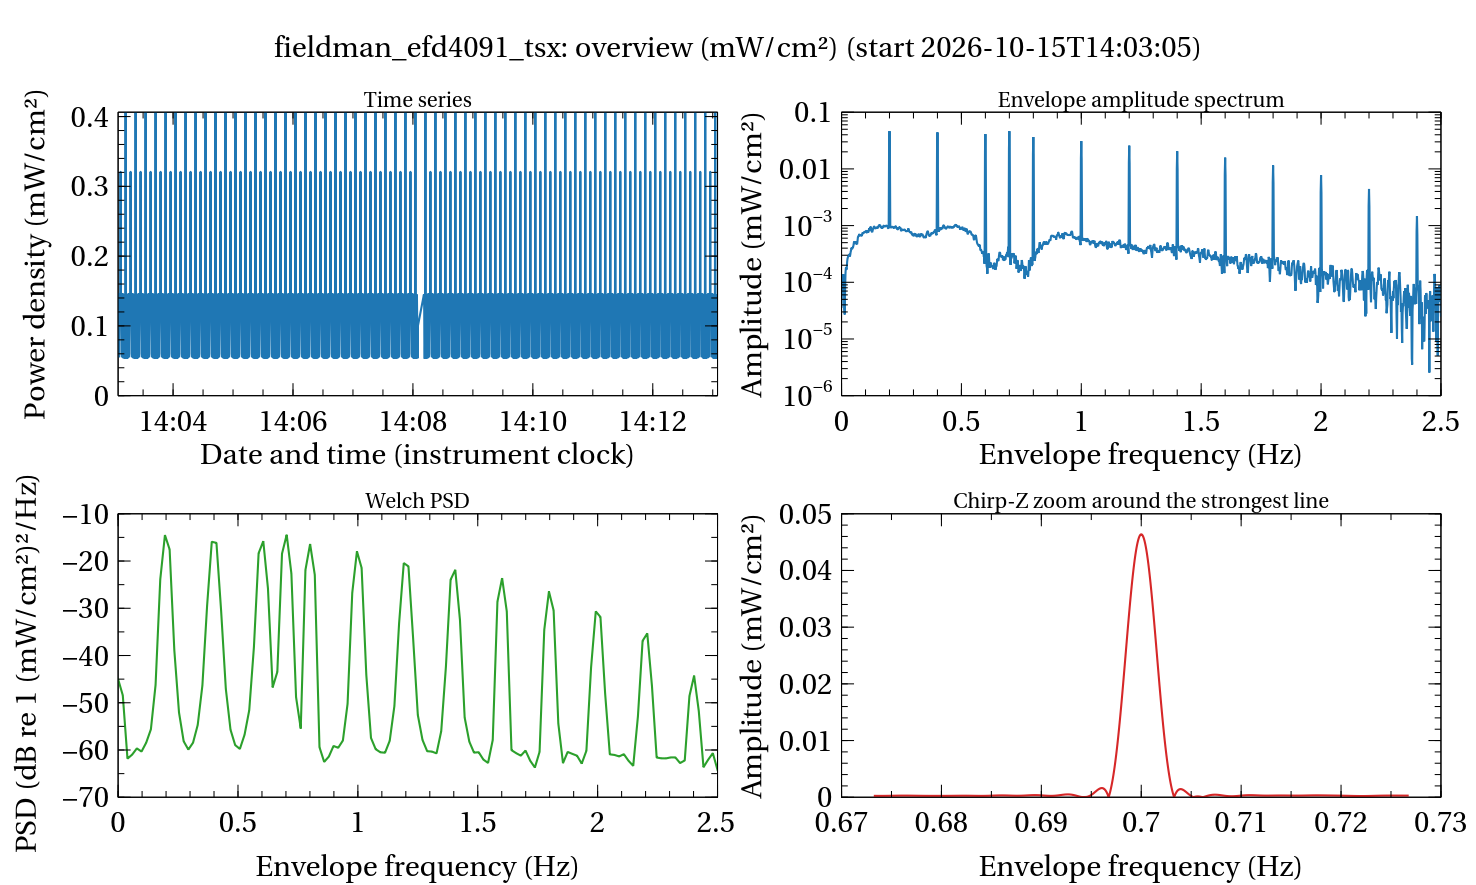
\includegraphics[width=0.92\linewidth]{figures/fig_overview.png}}{\fbox{\parbox{0.8\linewidth}{\centering Figure file \path{figures/fig_overview.png} not found: run \path{tools/build_manual_pdf.py --figures}.}}}
\caption{Veusz overview page: time series, amplitude spectrum, Welch PSD and chirp-Z zoom of one log. \emph{(Synthetic data.)}}\label{fig:overview}
\end{figure}

\begin{figure}[htbp]
\centering
\IfFileExists{figures/fig_fieldman_time.png}{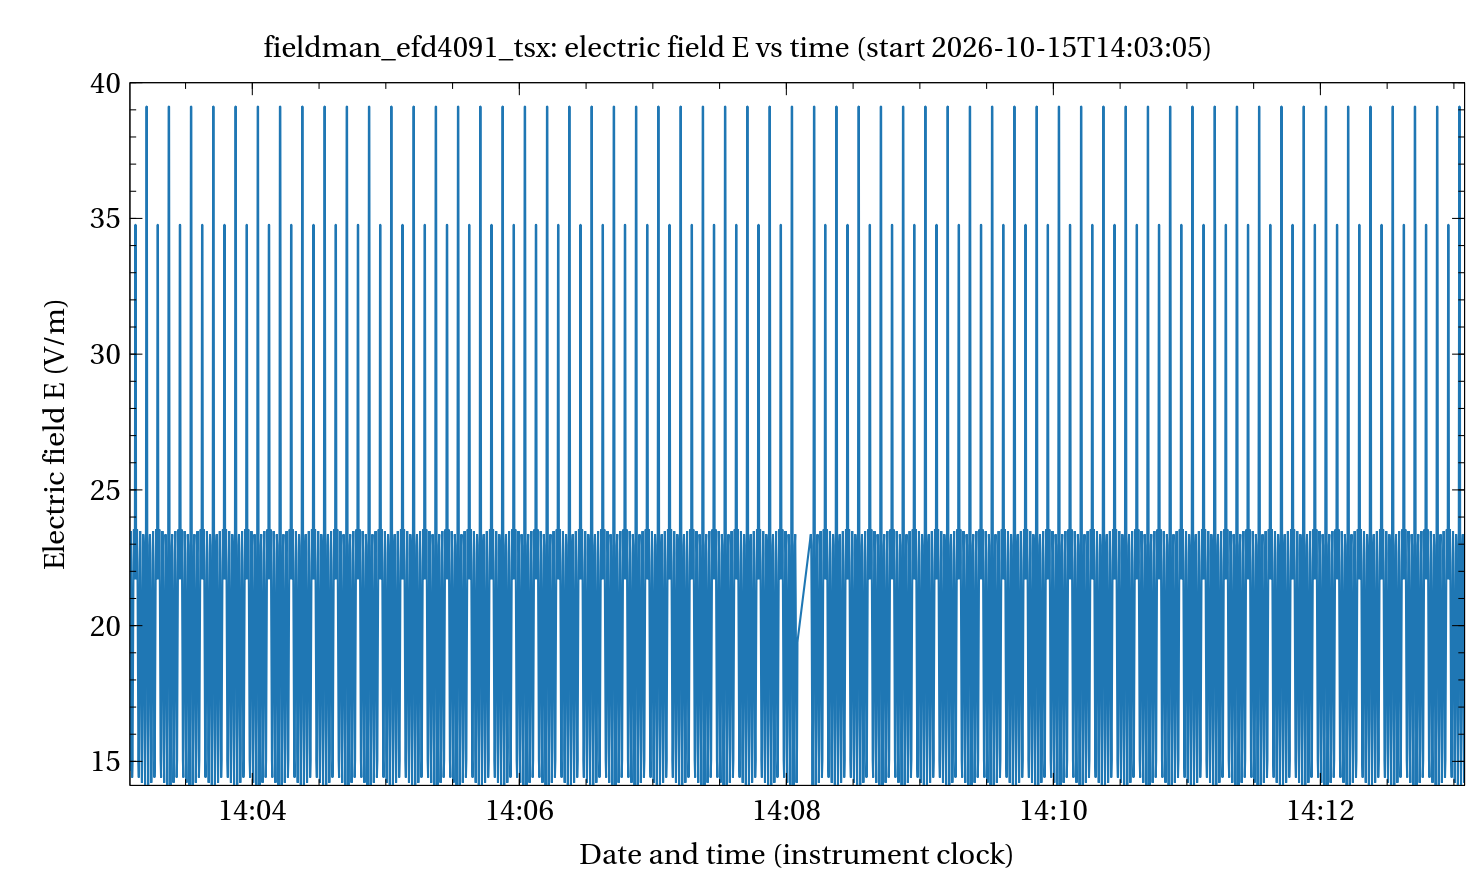
\includegraphics[width=0.92\linewidth]{figures/fig_fieldman_time.png}}{\fbox{\parbox{0.8\linewidth}{\centering Figure file \path{figures/fig_fieldman_time.png} not found: run \path{tools/build_manual_pdf.py --figures}.}}}
\caption{Synthetic FieldMan/Narda-TSX log (EFD-4091): field against the instrument clock on a date axis. The 6\,s gap at 300\,s is deliberate. \emph{(Synthetic data.)}}\label{fig:time}
\end{figure}

\begin{figure}[htbp]
\centering
\IfFileExists{figures/fig_fieldman_amplitude.png}{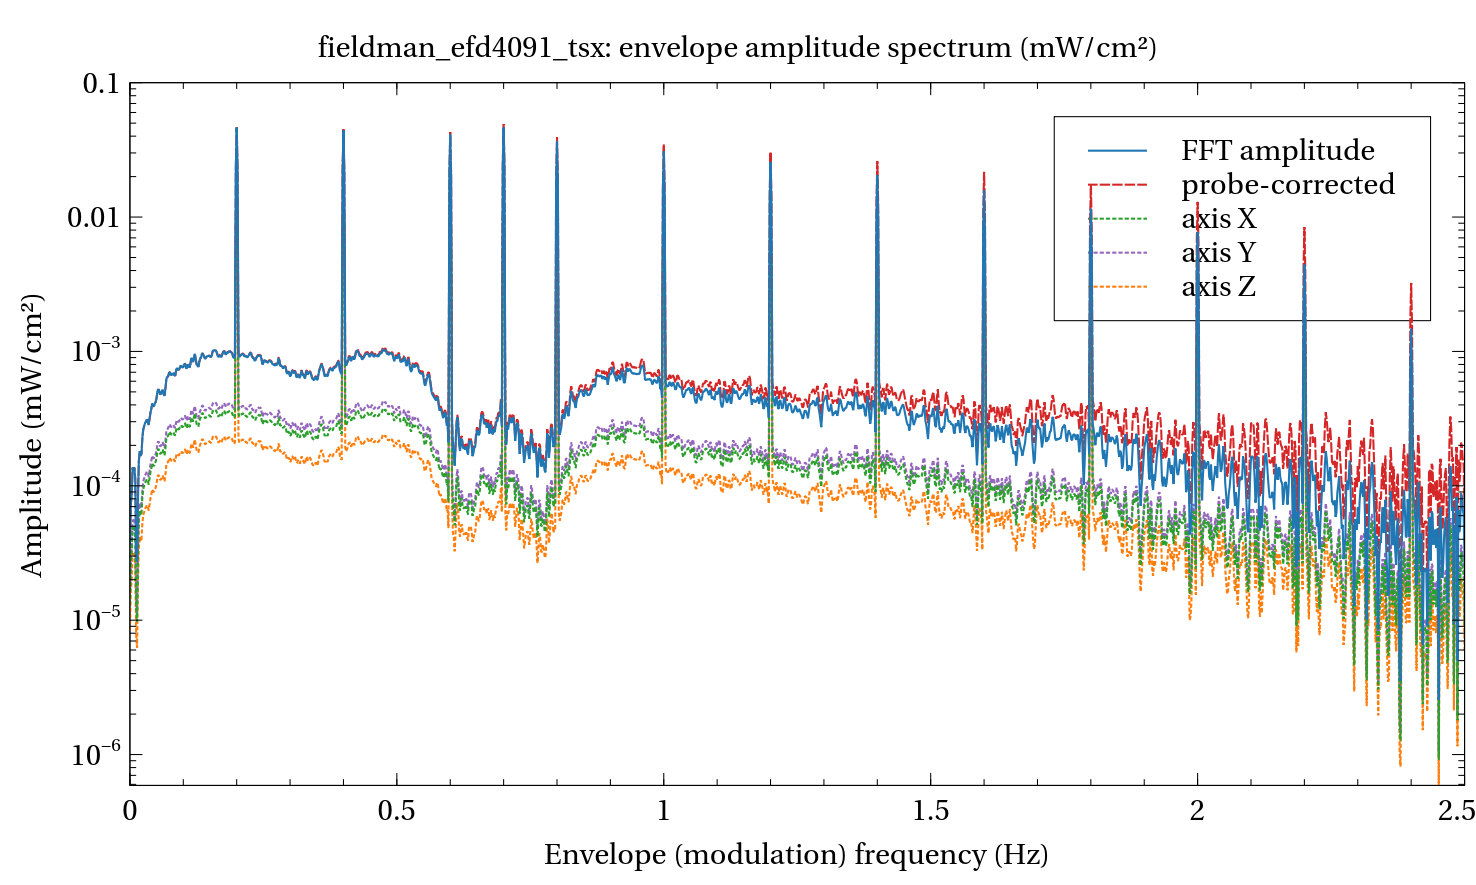
\includegraphics[width=0.92\linewidth]{figures/fig_fieldman_amplitude.png}}{\fbox{\parbox{0.8\linewidth}{\centering Figure file \path{figures/fig_fieldman_amplitude.png} not found: run \path{tools/build_manual_pdf.py --figures}.}}}
\caption{Envelope amplitude spectrum of the same log: the 12\,rpm radar family (0.2\,Hz and harmonics), the 0.7\,Hz source, the probe-corrected trace (dashed) and the X/Y/Z axes (dotted). \emph{(Synthetic data.)}}\label{fig:amplitude}
\end{figure}

\begin{figure}[htbp]
\centering
\IfFileExists{figures/fig_fieldman_zoom.png}{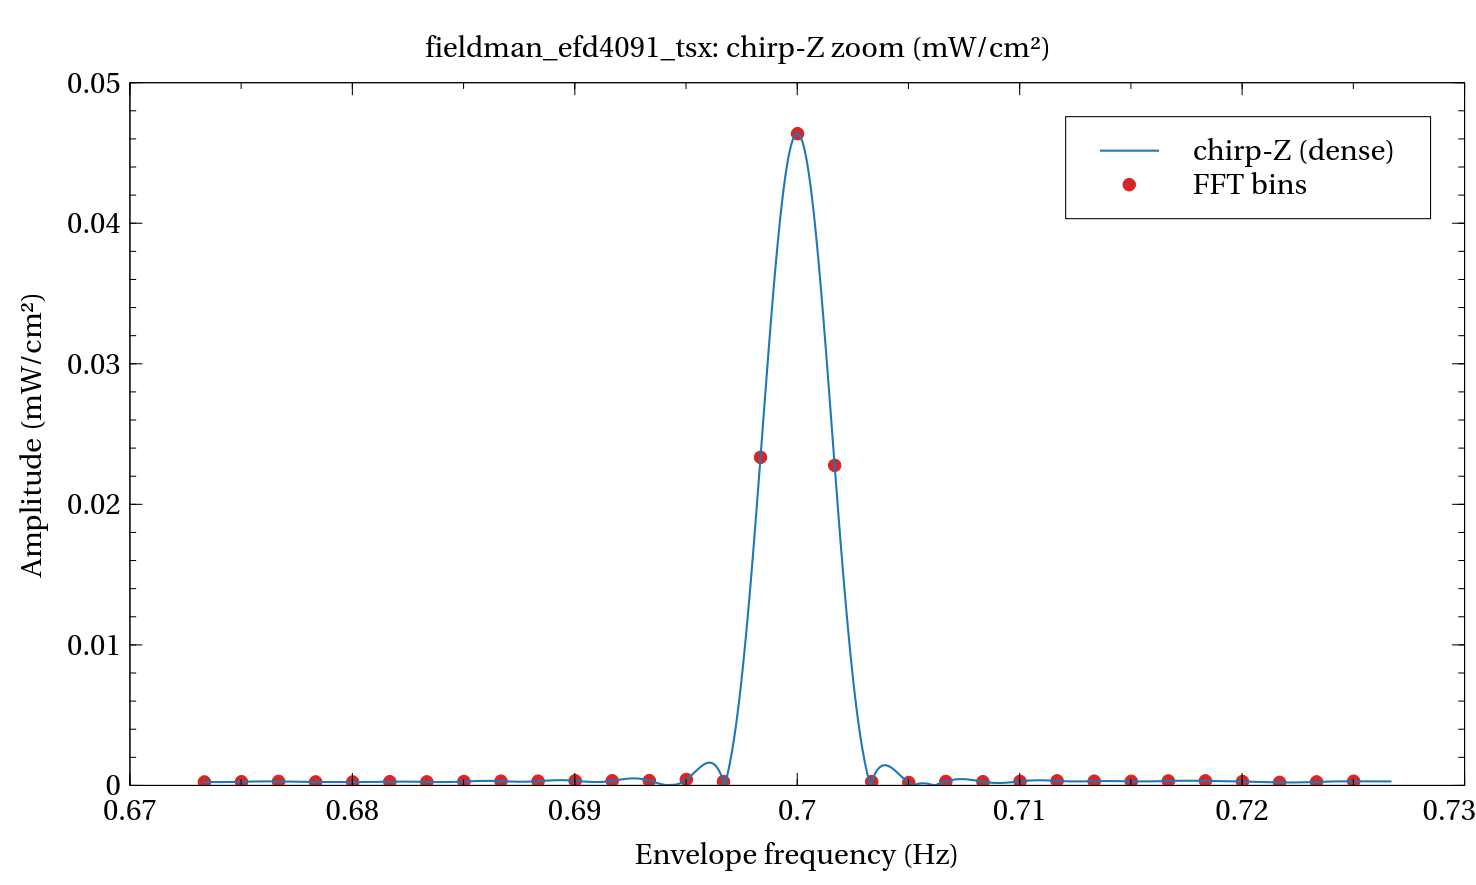
\includegraphics[width=0.92\linewidth]{figures/fig_fieldman_zoom.png}}{\fbox{\parbox{0.8\linewidth}{\centering Figure file \path{figures/fig_fieldman_zoom.png} not found: run \path{tools/build_manual_pdf.py --figures}.}}}
\caption{Chirp-Z zoom around the strongest line: the dense CZT samples (line) between the FFT bins (markers). \emph{(Synthetic data.)}}\label{fig:zoom}
\end{figure}

\begin{figure}[htbp]
\centering
\IfFileExists{figures/fig_fieldman_probe.png}{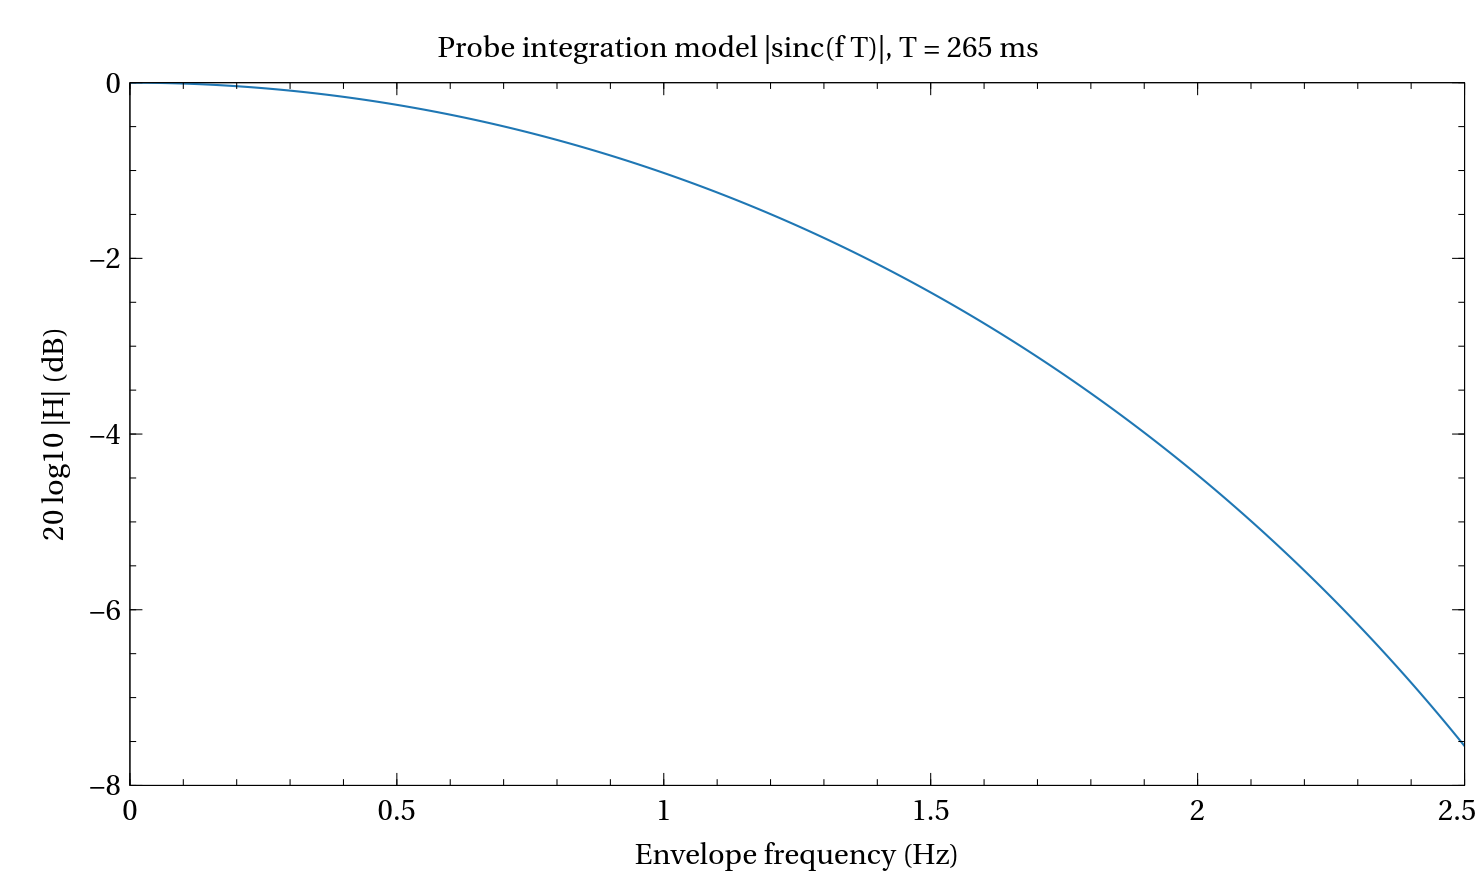
\includegraphics[width=0.92\linewidth]{figures/fig_fieldman_probe.png}}{\fbox{\parbox{0.8\linewidth}{\centering Figure file \path{figures/fig_fieldman_probe.png} not found: run \path{tools/build_manual_pdf.py --figures}.}}}
\caption{Probe integration model $|H(\nu)| = |\operatorname{sinc}(\nu T)|$ for $T = 265$\,ms up to the Nyquist frequency. \emph{(Synthetic data.)}}\label{fig:probe}
\end{figure}

\begin{figure}[htbp]
\centering
\IfFileExists{figures/fig_signalshark_spectrogram.png}{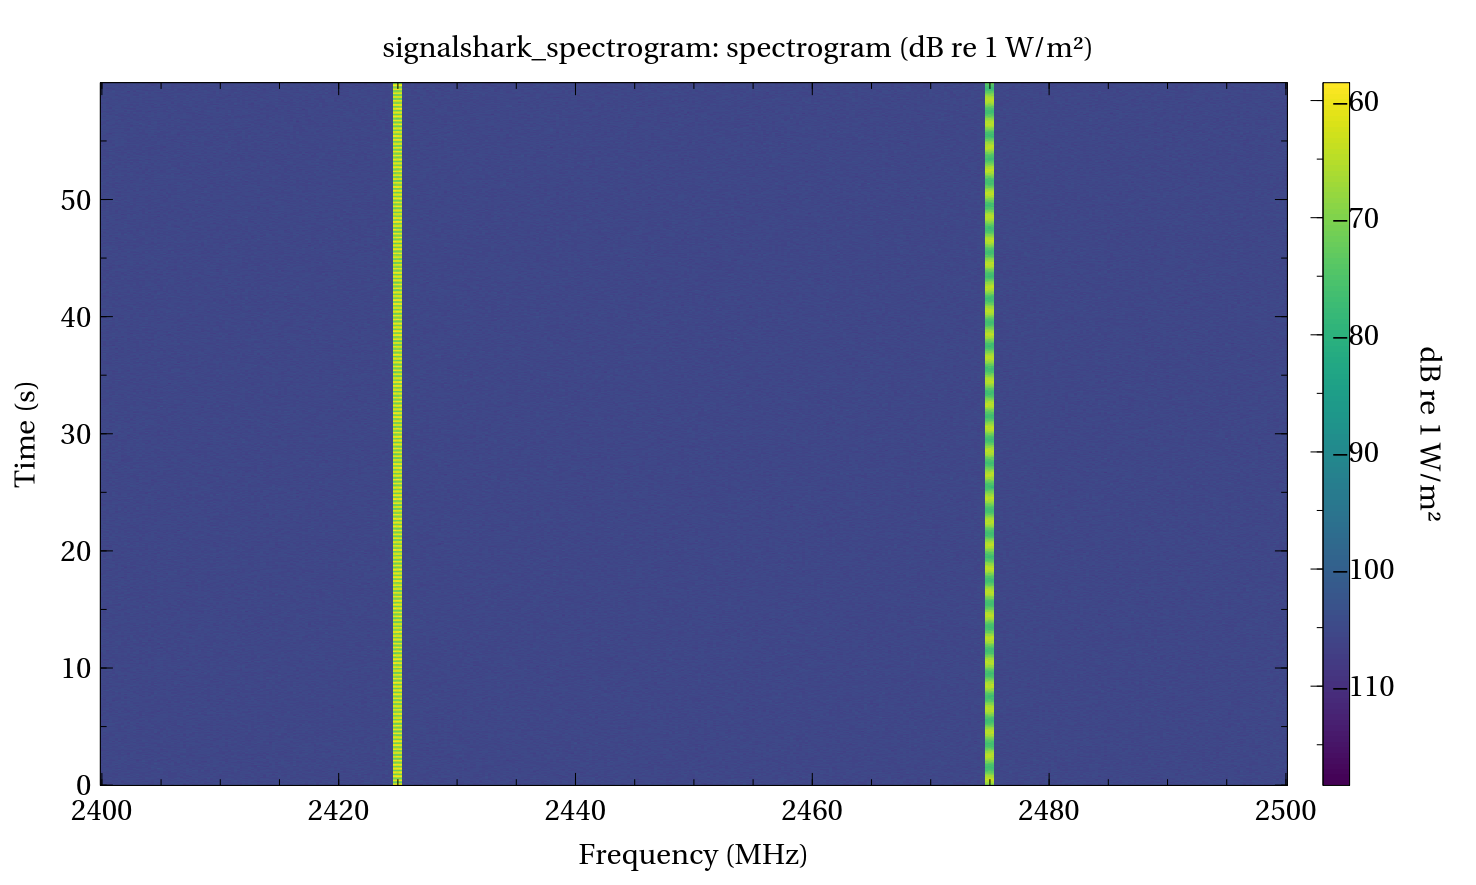
\includegraphics[width=0.92\linewidth]{figures/fig_signalshark_spectrogram.png}}{\fbox{\parbox{0.8\linewidth}{\centering Figure file \path{figures/fig_signalshark_spectrogram.png} not found: run \path{tools/build_manual_pdf.py --figures}.}}}
\caption{Synthetic SignalShark spectrogram: two carriers whose levels vary at 3\,Hz and 0.5\,Hz. \emph{(Synthetic data.)}}\label{fig:spectrogram}
\end{figure}

\begin{figure}[htbp]
\centering
\IfFileExists{figures/fig_signalshark_modulation_map.png}{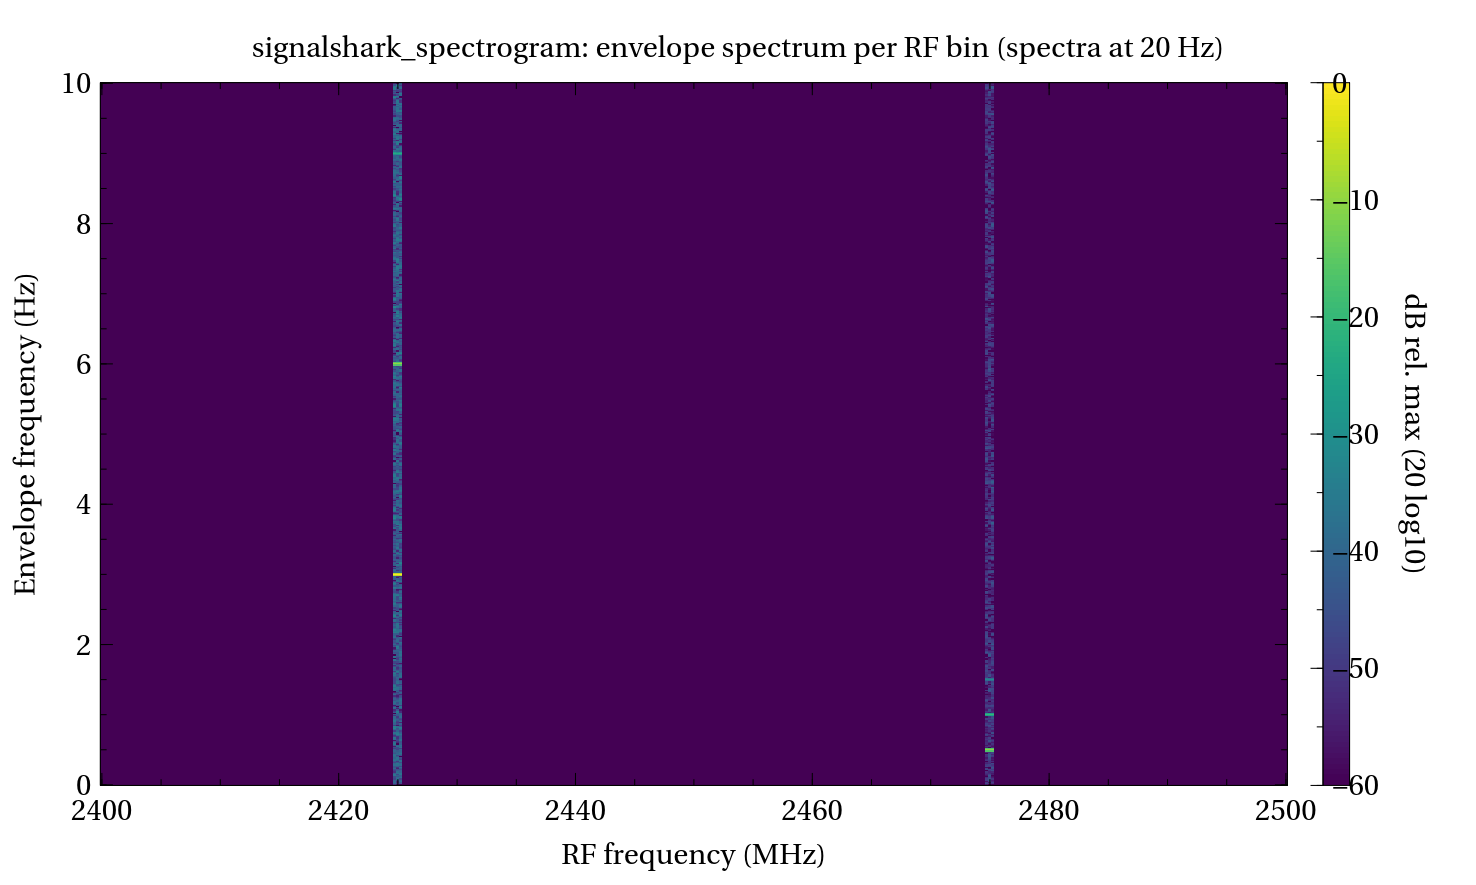
\includegraphics[width=0.92\linewidth]{figures/fig_signalshark_modulation_map.png}}{\fbox{\parbox{0.8\linewidth}{\centering Figure file \path{figures/fig_signalshark_modulation_map.png} not found: run \path{tools/build_manual_pdf.py --figures}.}}}
\caption{Envelope spectrum of every RF bin of that spectrogram: each carrier shows its own modulation frequency. \emph{(Synthetic data.)}}\label{fig:modmap}
\end{figure}

\begin{figure}[htbp]
\centering
\IfFileExists{figures/fig_units_time.png}{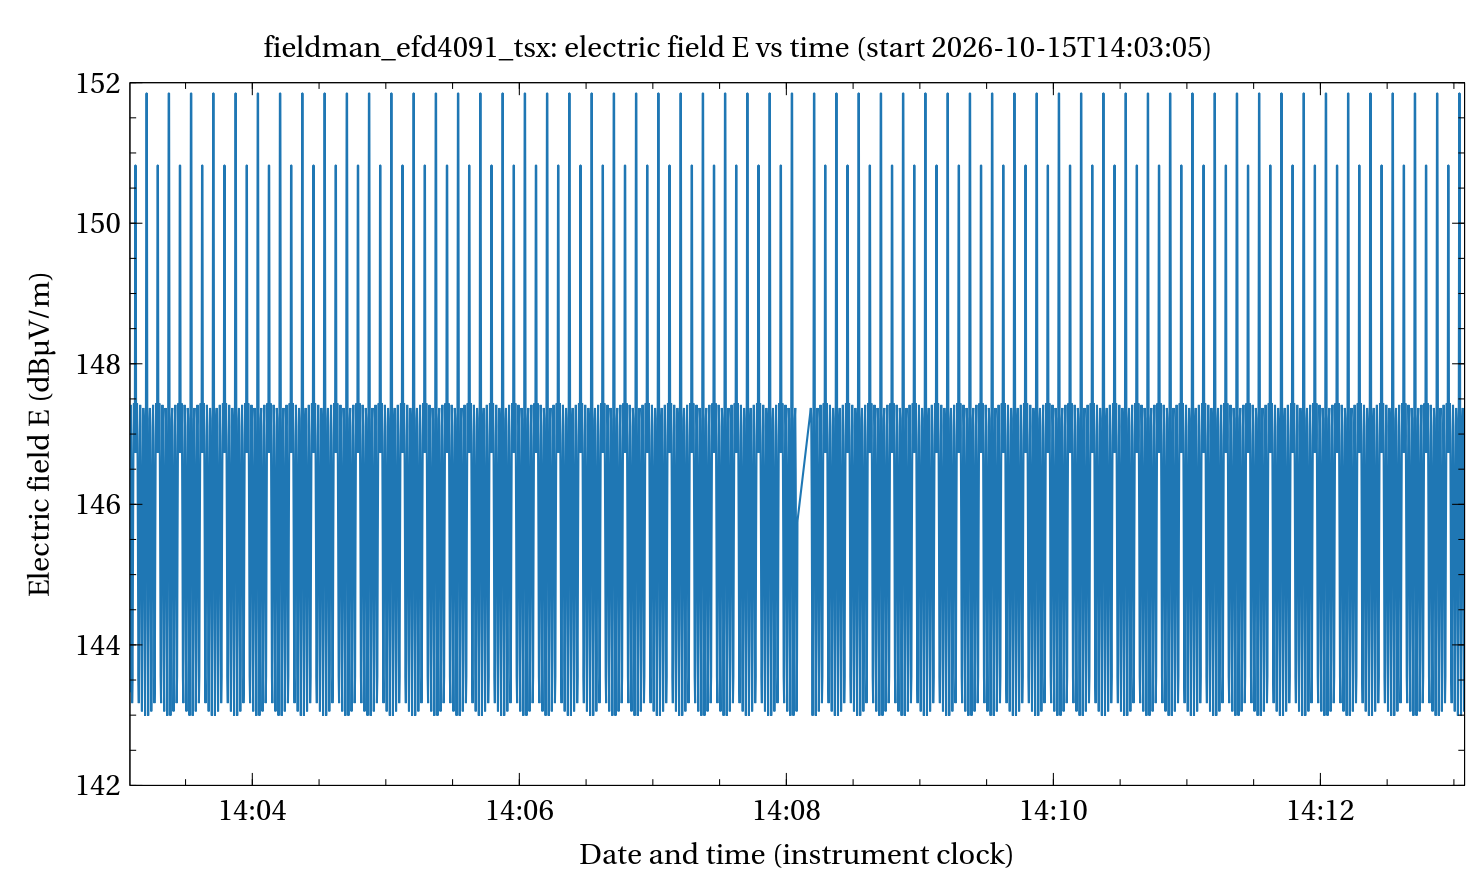
\includegraphics[width=0.92\linewidth]{figures/fig_units_time.png}}{\fbox{\parbox{0.8\linewidth}{\centering Figure file \path{figures/fig_units_time.png} not found: run \path{tools/build_manual_pdf.py --figures}.}}}
\caption{Logged field of the same log shown as $E$ in dB\textmu V/m (display units \texttt{mW/cm2,dBuV/m}). \emph{(Synthetic data.)}}\label{fig:units_time}
\end{figure}

\begin{figure}[htbp]
\centering
\IfFileExists{figures/fig_units_amplitude_dbm.png}{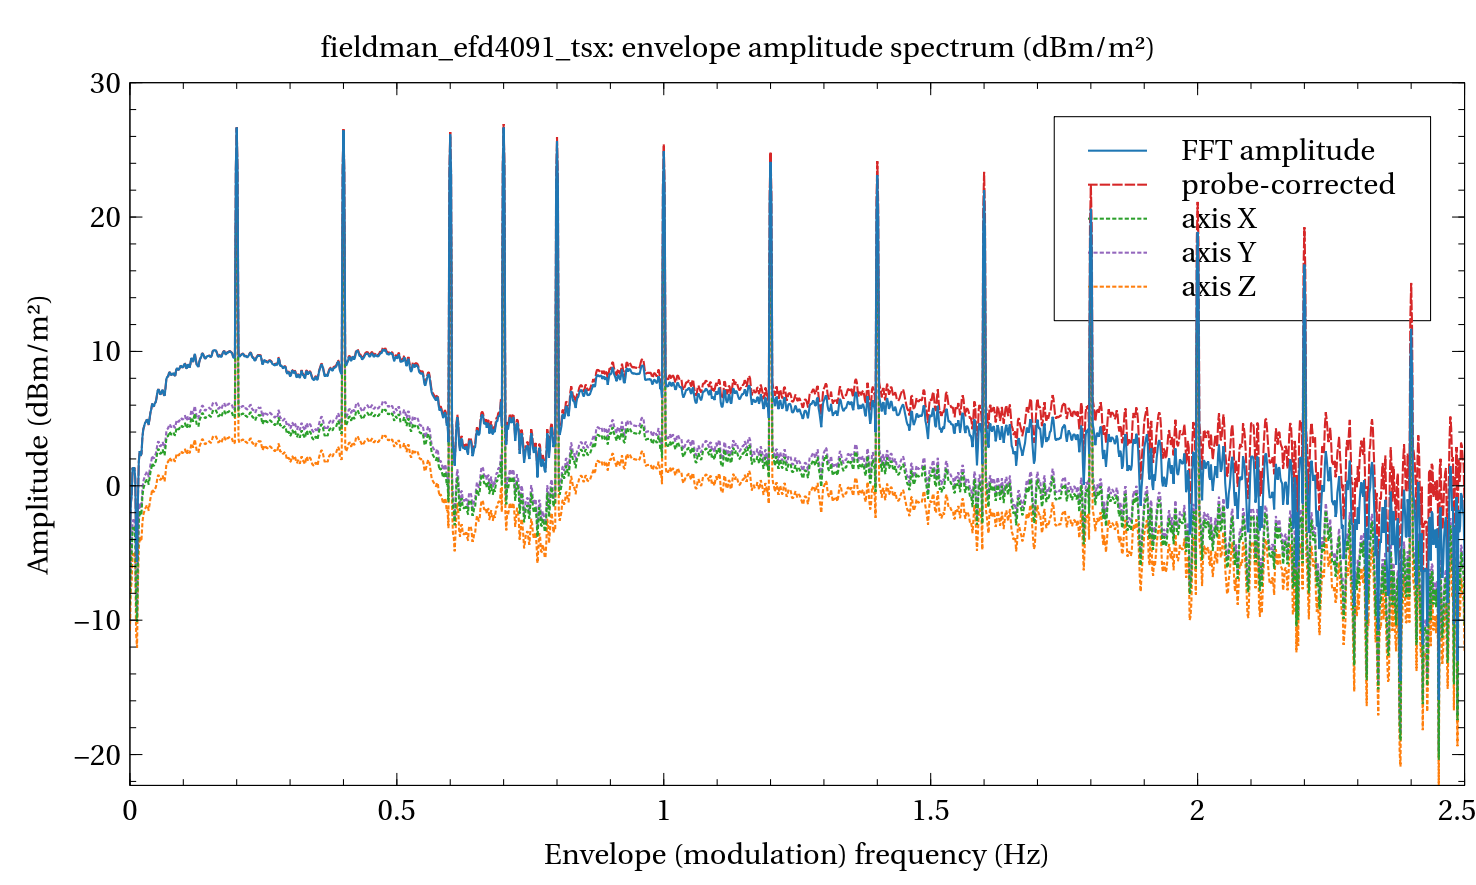
\includegraphics[width=0.92\linewidth]{figures/fig_units_amplitude_dbm.png}}{\fbox{\parbox{0.8\linewidth}{\centering Figure file \path{figures/fig_units_amplitude_dbm.png} not found: run \path{tools/build_manual_pdf.py --figures}.}}}
\caption{Page of an extra unit section (\texttt{--veusz-units dBm/m2}): the amplitude spectrum in dBm/m$^2$, $10\log_{10}$ of the amplitude in mW/m$^2$, on a linear axis. \emph{(Synthetic data.)}}\label{fig:units_amplitude}
\end{figure}

\begin{figure}[htbp]
\centering
\IfFileExists{figures/fig_units_hfield.png}{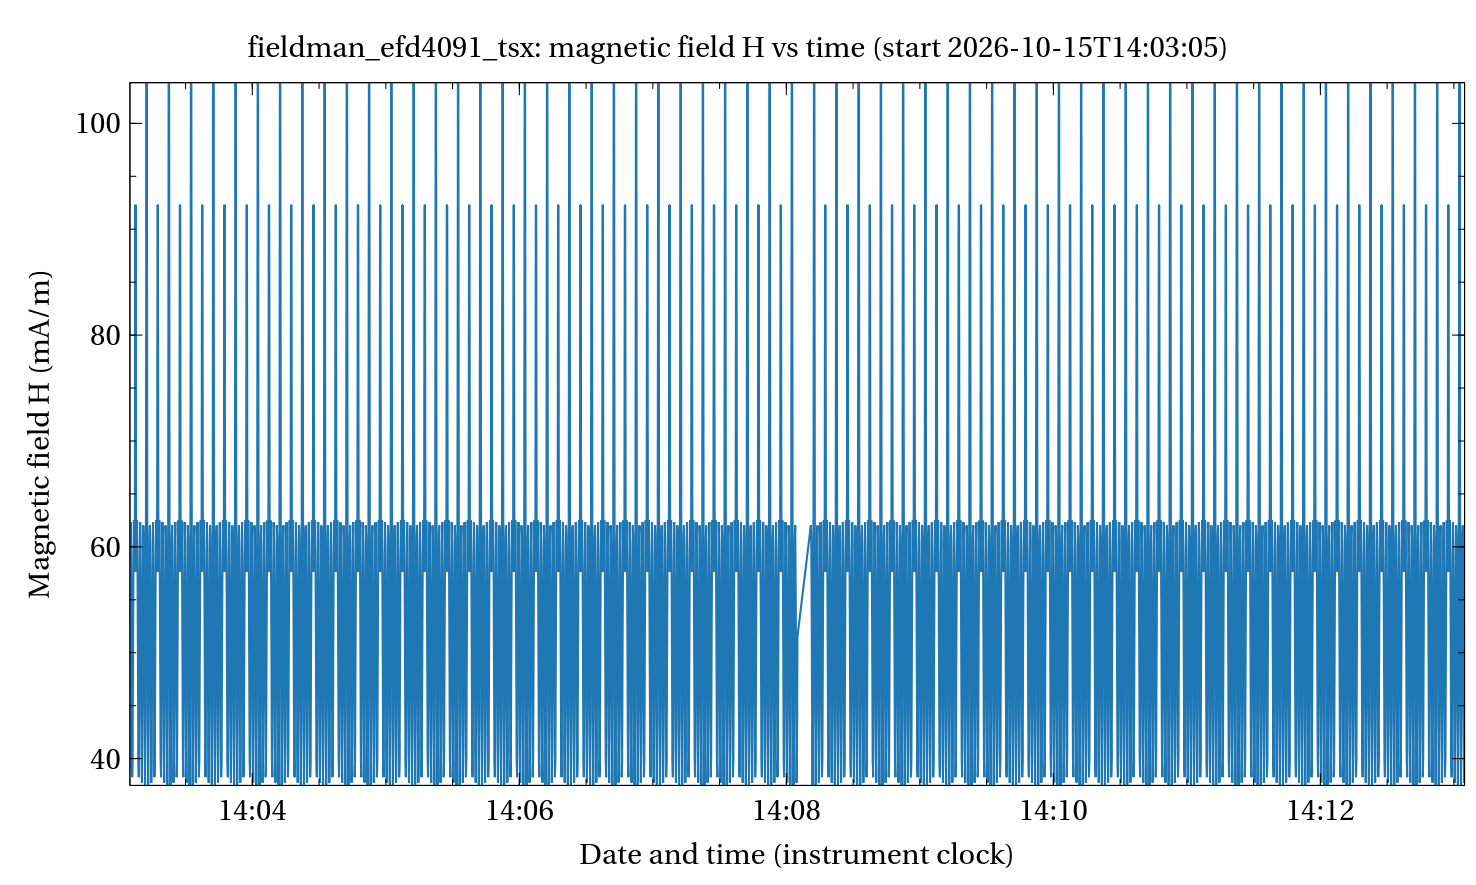
\includegraphics[width=0.92\linewidth]{figures/fig_units_hfield.png}}{\fbox{\parbox{0.8\linewidth}{\centering Figure file \path{figures/fig_units_hfield.png} not found: run \path{tools/build_manual_pdf.py --figures}.}}}
\caption{Page of the \texttt{mA/m} section: $H=\sqrt{S/Z_0}$ of the equivalent plane wave against time. \emph{(Synthetic data.)}}\label{fig:units_hfield}
\end{figure}

\clearpage

% =============================================================================
%    8  LIVE MODE
% =============================================================================
\section{Live mode}\label{sec:live}
The \emph{Live} tab of the GUI (or \texttt{--live FILE}) follows a text file that
another program appends to. New
complete lines are read every \texttt{--update} seconds (default 1\,s; an
unfinished last line waits for the next poll), kept in a ring buffer twice the
size of the analysis window \texttt{--window-s} (default 120\,s), and the
envelope amplitude spectrum and Welch PSD of the latest window are recomputed
and drawn. Every sample is also appended to \path{<file>.live.f64}, raw float64
pairs (time, value) that can be read back with
\verb|np.fromfile(path).reshape(-1, 2)|. The plots follow the unit control of
the settings panel exactly as the Analysis tab does: the time plot in the
\emph{Time plot shows} mode, the spectra in the unit of the analysed quantity's
family, the PSD in dB re 1\,(unit)$^2$/Hz, re-plotted at once when a unit
changes; the console mode (\texttt{--no-gui}) prints the peak amplitudes in that
unit. \emph{Save snapshot} analyses the current window fully and writes the
usual output files, including the extra Veusz units and layout, and \emph{Clear buffer} empties the RAM buffer (the disk
log keeps every sample). \texttt{--no-gui} prints the strongest lines and families
instead; \texttt{--live-seconds} stops after a time.

Neither FieldMan nor Narda-TSX documents a continuously written file or a
streaming interface for the broadband probes \cite{R5,R9}, so whether live mode
works with them depends on how they write data; it was tested with a file
written in real time by a script. NBM-550 remote output (\texttt{MEAS\_START},
5, 50 or 60 samples per second \cite{R6}) logged to a file by another tool is a
documented route.

\begin{figure}[htbp]
\centering
\IfFileExists{figures/fig_gui_live.png}{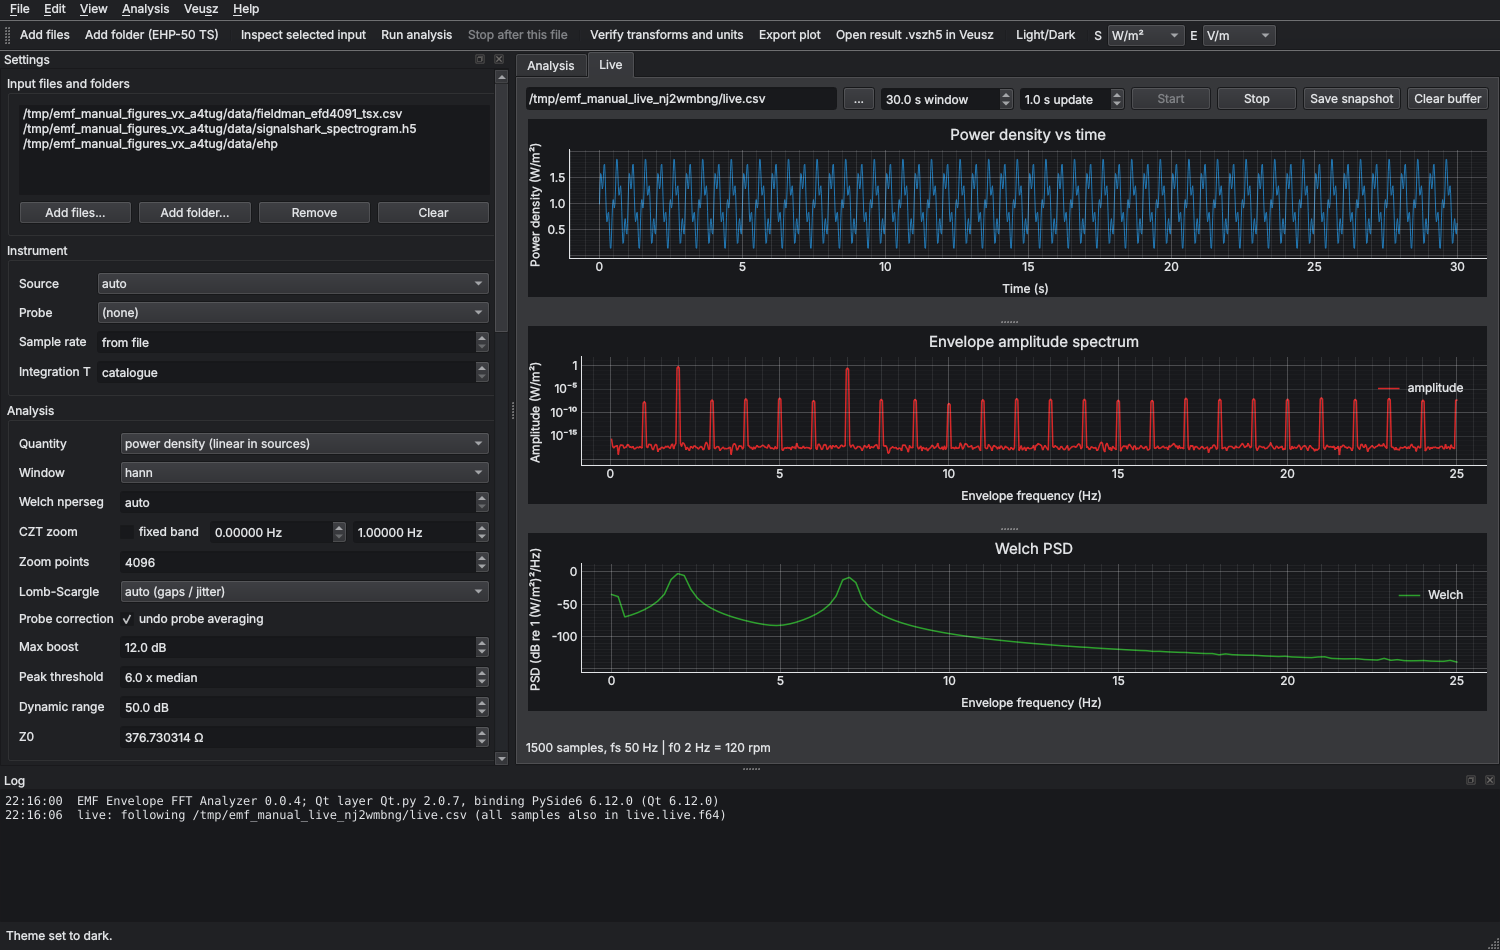
\includegraphics[width=0.92\linewidth]{figures/fig_gui_live.png}}{\fbox{\parbox{0.8\linewidth}{\centering Figure file \path{figures/fig_gui_live.png} not found: run \path{tools/build_manual_pdf.py --figures}.}}}
\caption{Live tab (dark theme) following a growing file with 2\,Hz and 7\,Hz envelope tones. \emph{(Synthetic data.)}}\label{fig:live}
\end{figure}


% =============================================================================
%    9  MEMORY, PARALLEL PROCESSING AND GPU
% =============================================================================
\section{Memory, parallel processing and GPU}\label{sec:memory}
\begin{itemize}
\item \textbf{Spill to disk}: a column longer than 20\,000\,000 samples is moved
from RAM to a temporary raw file and used as a memory map; the files are
deleted when the program exits. A 2.4-million-row, 900\,Hz test log was
analysed this way.
\item \textbf{Chunks and batches}: text files are read 500\,000 rows at a time;
Welch processes 512 segments at a time; Lomb--Scargle about 64\,MiB of
frequencies at a time; the per-bin modulation spectra in batches of about
256\,MiB.
\item \textbf{Freeing memory}: \texttt{flush\_memory()} runs the garbage
collector and empties the CuPy memory pools; batch mode calls it after each
file and after every GUI analysis run, and so do the \emph{Clear buffer} button of
the Live tab (empties the ring buffer; the disk log is kept) and \emph{Edit
$\rightarrow$ Free memory} (forgets the results shown and empties the live buffer).
\texttt{--pickle} also writes the whole result object to
\path{<stem>_result.pkl} (load it with \texttt{load\_pickle}, only from files you
trust).
\item \textbf{Parallel}: \texttt{--jobs N} analyses N files in separate processes;
each process then uses one FFT thread so that the cores are not
oversubscribed. With one job, SciPy's FFTs use every core.
\item \textbf{GPU}: \texttt{--gpu} moves the FFTs, Welch segments, modulation
spectra and Lomb--Scargle sums to an NVIDIA GPU through CuPy \cite{B27}. Without
CuPy or a CUDA device the program continues on the CPU and says why in the
summary (\texttt{backend}).
\end{itemize}

% =============================================================================
%    10  WORKING IN SPYDER
% =============================================================================
\section{Working in Spyder}\label{sec:spyder}
The script is organised in Spyder cells, each opened by a banner
\verb|# %% ====| and a title line. Table~\ref{tab:cells} lists them with the
functions and classes each defines (generated from the script). Run the cells
from the top; the last cell is a commented scratch cell:
\begin{Verbatim}
opts = Options(probe="EFD-4091", correct_probe=True, lomb="on",
               display_unit="mW/cm2,dBuV/m", veusz_units="dBm/m2,mA/m")
print(inspect_input(r"C:\path\to\export.csv", opts))
series = load_any(r"C:\path\to\export.csv", opts)
result = analyse_timeseries(series, opts)
print(result.peaks[:5], result.families)
print("\n".join(summary_lines(result, "uW/cm2,dBuV/m")))
write_outputs(result, Path(r"C:\path\to\out"), opts)
opts.veusz_units, opts.veusz_layout = "W/m2,uW/cm2", "files"     # other units,
write_veusz(result, Path(r"C:\path\to\out"), opts)             # no re-analysis
print_unit_table()
flush_memory()
\end{Verbatim}

\begingroup\footnotesize
\begin{longtable}{@{}L{\dimexpr 0.06\linewidth-2\tabcolsep\relax}L{\dimexpr 0.27\linewidth-2\tabcolsep\relax}L{\dimexpr 0.07\linewidth-2\tabcolsep\relax}L{\dimexpr 0.58\linewidth-2\tabcolsep\relax}@{}}
\caption{Spyder cells of emf\_envelope\_fft\_v0\_0\_4.py.}\label{tab:cells}\\
\toprule
\textbf{No.} & \textbf{Cell} & \textbf{Line} & \textbf{Definitions} \\
\midrule
\endfirsthead
\multicolumn{4}{@{}l}{\itshape\footnotesize Table \thetable{} (continued)}\\
\toprule
\textbf{No.} & \textbf{Cell} & \textbf{Line} & \textbf{Definitions} \\
\midrule
\endhead
\bottomrule
\endlastfoot
1 & MODULE HEADER & 6 & \textit{(constants, imports or comments)} \\
2 & IMPORTS & 329 & \textit{(constants, imports or comments)} \\
3 & CONSTANTS, PROBE CATALOGUE AND UNITS & 392 & ProbeSpec, lookup\_probe, parse\_unit, to\_power\_like, to\_field\_like, DisplayUnit, UnitFamily, lookup\_display\_unit, \_split\_units, ... (32 in all) \\
4 & DATA MODEL & 1036 & TimeSeries, SpectrumSet, Options \\
5 & MEMORY HELPERS (bounded RAM for long logs) & 1140 & \_remove\_spill\_files, SpillBuffer, flush\_memory, save\_pickle, load\_pickle \\
6 & COMPUTE BACKEND (CPU / optional GPU) & 1253 & Backend \\
7 & TEXT EXPORT SNIFFING AND READING & 1294 & TextLayout, \_read\_head, \_is\_number, \_split, sniff\_text, \_pick\_columns, TimeOrigin, \_to\_seconds, \_origin\_text, ... (23 in all) \\
8 & PRE-PROCESSING: TIMING, GAPS, UNIFORM GRID & 1967 & UniformSeries, make\_uniform, analysis\_quantity \\
9 & SPECTRAL ESTIMATORS & 2049 & amplitude\_spectrum, welch\_blocks, czt\_zoom, lomb\_scargle, envelope\_spectrogram, modulation\_spectra, probe\_response, correction\_gain, correct\_probe \\
10 & PEAKS AND HARMONIC FAMILIES & 2229 & find\_spectral\_peaks, harmonic\_families \\
11 & ANALYSIS DRIVERS & 2296 & SeriesResult, \_default\_nperseg, analyse\_timeseries, SpectrogramResult, \_decimate\_max, analyse\_spectrumset \\
12 & VEUSZ .vszh5 OUTPUT (through the author's vszh5\_writer.py) & 2632 & \_freq\_unit, \_outline\_for, bookmark\_outline, UnitView, primary\_view, \_focus\_view, veusz\_views, safe\_unit\_tag, \_result\_units, ... (23 in all) \\
13 & OTHER OUTPUTS: CSV, NPZ, JSON SUMMARY, OPTIONAL RENDER & 3292 & \_summary\_series, \_summary\_spectrogram, \_jsonable, \_write\_csv, write\_outputs, write\_veusz, render\_documents, render\_vszh5 \\
14 & BATCH (PARALLEL) PROCESSING & 3451 & analyse\_path, output\_folder, analyse\_and\_write, process\_file, process\_files \\
15 & LIVE MODE: FOLLOW A GROWING FILE & 3519 & LiveTail, RingBuffer, live\_update, live\_record, \_live\_ring, run\_live\_console \\
16 & GUI: QT BINDING (Qt.py or QtPy abstraction layer, PySide6 binding) & 3711 & \_QtMissingMeta, \_QtMissing, \_import\_qt \\
17 & GUI: THEME MANAGER (light / dark / system, as in the QuickSyn controller) & 3804 & ThemeManager \\
18 & GUI: SMALL WIDGETS AND HELPERS & 3890 & make\_double\_spin, make\_int\_spin, make\_combo, import\_qt\_module, export\_widget\_svg, monospace\_font, \_finite\_positive \\
19 & GUI: PLOT PANELS (pyqtgraph) & 3978 & PlotPanel, ImagePanel \\
20 & GUI: BACKGROUND TASKS (analysis, inspect, verification in a QThread) & 4231 & TaskThread, analysis\_job \\
21 & GUI: SETTINGS PANEL (inputs, analysis options, output, display units) & 4300 & SettingsPanel \\
22 & GUI: RESULTS VIEW (plots, peaks, summary, inspect, verification) & 4750 & ResultsView \\
23 & GUI: LIVE PANEL (follow a growing file) & 5070 & LivePanel \\
24 & GUI: ABOUT DIALOG CONTENT & 5254 & \_module\_version, build\_about\_content \\
25 & GUI: MAIN WINDOW & 5323 & MainWindow \\
26 & GUI: ENTRY POINT & 6115 & launch\_gui, run\_live\_gui \\
27 & VERIFICATION OF TRANSFORMS AND UNIT CONVERSIONS (0.0.3) & 6177 & Check, verify\_transforms \\
28 & SELF-TEST WITH SYNTHETIC EXPORTS & 6543 & \_synthetic\_radar, \_probe\_filter, make\_synthetic\_files, self\_test \\
29 & COMMAND LINE & 6751 & build\_parser, options\_from\_args, \_unit\_list\_argument, print\_unit\_table, main \\
30 & INTERACTIVE SCRATCH CELL (Spyder) & 6906 & \textit{(constants, imports or comments)} \\
\end{longtable}
\endgroup


% =============================================================================
%    11  VERIFICATION
% =============================================================================
\section{Verification}\label{sec:verification}
\texttt{--selftest} checks the estimators against known answers and then runs
every reader on synthetic files written in the styles expected from the
instruments (semicolon and decimal comma with German dates, a 1\,s NBM timer
log, an EHP-50 TS folder, a SignalShark-like HDF5 file and a converter CSV).
Table~\ref{tab:selftest} is the result of the run made while building this
manual.

\begingroup\footnotesize
\begin{longtable}{@{}L{\dimexpr 0.42\linewidth-2\tabcolsep\relax}L{\dimexpr 0.42\linewidth-2\tabcolsep\relax}L{\dimexpr 0.1\linewidth-2\tabcolsep\relax}@{}}
\caption{Self-test result (program 0.0.4, run during this build).}\label{tab:selftest}\\
\toprule
\textbf{Check} & \textbf{Measured} & \textbf{Result} \\
\midrule
\endfirsthead
\multicolumn{3}{@{}l}{\itshape\footnotesize Table \thetable{} (continued)}\\
\toprule
\textbf{Check} & \textbf{Measured} & \textbf{Result} \\
\midrule
\endhead
\bottomrule
\endlastfoot
streamed Welch == scipy.signal.welch & max rel err 3.6e-15 & PASS \\
FFT amplitude of 0.8 sinusoid & 0.802 & PASS \\
CZT peak frequency & 0.21000 Hz & PASS \\
Lomb-Scargle amplitude and frequency & 0.799 at 0.2100 Hz & PASS \\
|sinc| at 1.5 Hz, T=265 ms & -2.39 dB & PASS \\
transform and unit verification (-\kern0pt-verify) & 54/54 checks & PASS \\
FieldMan/TSX & radar 12 rpm family: [12.0, 42.0] & PASS \\
FieldMan/TSX & 0.7 Hz source found & PASS \\
NBM timer log & 6 rpm: [6.0] & PASS \\
EHP-50 TS spectra folder & 0.05 Hz modulation of 50 Hz line: [0.05, 0.05] & PASS \\
signalshark & per-channel envelope 0.5 and 3 Hz: [0.5, 3.0] & PASS \\
signalshark\_csv & per-channel envelope 0.5 and 3 Hz: [0.5, 3.0] & PASS \\
.vszh5 layout (Veusz format 1) & signalshark\_converted\_envelope\_fft.vszh5 & PASS \\
Veusz sections & W/m2, dBm/m2 and mA/m sections in one document: 42 datasets; sections ['Display units: mW/cm², dBµV/m', 'In W/m² (Power density)', 'In dBm/m² (Power density)', 'In mA/m (Magnetic field H)'] & PASS \\
Veusz values in mW/cm2 (x0.1) and dBm/m2 (10 log10(x1e3)) at the strongest line & 0.04637 mW/cm2, 26.6624 dBm/m2 & PASS \\
bookmarks grouped per unit section & ['Display units: mW/cm², dBµV/m', 'In W/m² (Power density)'] & PASS \\
Veusz one document per unit & fieldman\_efd4091\_tsx\_envelope\_fft.vszh5, fieldman\_efd4091\_tsx\_envelope\_fft\_Wm2.vszh5, fieldman\_efd4091\_tsx\_envelope\_fft\_dBmm2.vszh5, fieldman\_efd4091\_tsx\_envelope\_fft\_mAm.vszh5 & PASS \\
\end{longtable}
\endgroup


\subsection{Verification of the transforms and unit conversions}\label{sec:verify_table}
\texttt{--verify} (also \emph{Analysis $\rightarrow$ Verify transforms and units} in
the GUI, and part of the self-test) checks every time-to-frequency transform and
every unit conversion three independent ways:
\begin{description}
\item[analytic] a signal whose answer is known exactly: on-bin sinusoids, a line
half a bin off, hand-worked unit values, the sinc of a moving average, a
Gaussian-RBW carrier;
\item[reference] an independent implementation: \texttt{scipy.signal.periodogram},
\texttt{welch}, \texttt{spectrogram} and \texttt{lombscargle} \cite{R10}, or a
brute-force DFT or DTFT sum;
\item[identity] a law the result must obey: Parseval's theorem, Lomb--Scargle
equal to the FFT on a uniform grid, the zoom equal to the FFT on the bin
frequencies, conversion round trips.
\end{description}
Table~\ref{tab:verify} is the result of the run made while building this manual
(54 checks). It found, and version 0.0.3 fixed: the Nyquist row of the
per-bin modulation spectra was doubled; the unit headers mW/m$^2$, \textmu W/m$^2$
and dB(\textmu V/m) were not recognised and dBm/m$^2$ was read as dBm; the dBm to
dB\textmu V constant was rounded to 107\,dB; the probe-correction gain jumped by
1.94\,dB. Version 0.0.4 added the group \emph{Display units}: spellings, hand-worked
values in every family, round trips of all 34 units, the 10/20\,dB level
rule, squared units, PSD offsets, the plane-wave relations $E/H = Z_0$ and
$E H = S$, the conversion of 1\,mW/cm$^2$ to $E$ and $H$, RF levels in dBm/m$^2$,
dB\textmu V/m and dBW, and the per-family unit selection.

\begingroup\scriptsize
\begin{longtable}{@{}L{\dimexpr 0.11\linewidth-2\tabcolsep\relax}L{\dimexpr 0.09\linewidth-2\tabcolsep\relax}L{\dimexpr 0.4\linewidth-2\tabcolsep\relax}L{\dimexpr 0.2\linewidth-2\tabcolsep\relax}L{\dimexpr 0.1\linewidth-2\tabcolsep\relax}L{\dimexpr 0.08\linewidth-2\tabcolsep\relax}@{}}
\caption{Verification of transforms and units (program 0.0.4, run during this build).}\label{tab:verify}\\
\toprule
\textbf{Group} & \textbf{Method} & \textbf{Check} & \textbf{Measured} & \textbf{Limit} & \textbf{Result} \\
\midrule
\endfirsthead
\multicolumn{6}{@{}l}{\itshape\footnotesize Table \thetable{} (continued)}\\
\toprule
\textbf{Group} & \textbf{Method} & \textbf{Check} & \textbf{Measured} & \textbf{Limit} & \textbf{Result} \\
\midrule
\endhead
\bottomrule
\endlastfoot
Units & analytic & parse\_unit on 25 header spellings & all recognised & all & PASS \\
Units & analytic & to\_power\_like: 14 hand-worked values (V/m, dBuV/m, W/m2, mW/cm2, A/m, ...) & 0.00e+00 & <= 1e-12 & PASS \\
Units & analytic & dBm -> dBuV (+106.99 dB, 50 ohm) -> + AF -> E\textasciicircum{}2/Z0 & 0.00e+00 & <= 1e-12 & PASS \\
Units & analytic & dBm without AF -> mW (0 dBm = 1 mW); dBuV -> uV\textasciicircum{}2 (20 dBuV = 100 uV\textasciicircum{}2) & 0.00e+00 & <= 1e-12 & PASS \\
Units & identity & round trip E -> S = E\textasciicircum{}2/Z0 -> E = sqrt(S Z0) & 9.19e-17 & <= 1e-12 & PASS \\
Units & analytic & E in dBuV/m: 1 V/m = 120, 1 mV/m = 60 & 0.00e+00 & <= 1e-09 & PASS \\
Units & analytic & display units: 1 W/m2 = 1e3 mW/m2 = 1e6 uW/m2 = 0.1 mW/cm2 = 100 uW/cm2 & 0.00e+00 & <= 1e-15 & PASS \\
Units & identity & display units of a PSD scale with the factor squared & 0.00e+00 & <= 1e-15 & PASS \\
Units & analytic & to\_field\_like: 1 mW/cm2 -> sqrt(10 Z0) = 61.38 V/m & 0.00e+00 & <= 1e-12 & PASS \\
Display units & analytic & lookup\_display\_unit on 13 spellings (µ/μ/u, \textasciicircum{}2/², dB(...)) & all recognised & all & PASS \\
Display units & analytic & 25 hand-worked values: 1 W/m2 = 0.1 mW/cm2 = 30 dBm/m2, 1 V/m = 120 dBuV/m, 1 mW = -30 dBW, ... & 0.00e+00 & <= 1e-12 & PASS \\
Display units & identity & round trip to\_display -> from\_display for all 34 units & 1.84e-15 & <= 1e-12 & PASS \\
Display units & analytic & level rule: x10 in value = +10 dB (power units), +20 dB (root-power units) & 0.00e+00 & <= 1e-12 & PASS \\
Display units & identity & squared quantities: (k x)\textasciicircum{}2 for linear units; dB re 1 (ref)\textasciicircum{}2 of x\textasciicircum{}2 = level of x & 2.84e-14 & <= 1e-12 & PASS \\
Display units & analytic & PSD in dB re 1 (unit)\textasciicircum{}2/Hz: mW/cm2 -20 dB, dBm/m2 (mW/m2) +60 dB, dBuV/m +120 dB & 0.00e+00 & <= 1e-12 & PASS \\
Display units & identity & plane wave: E/H = Z0 and E x H = S for the time-plot conversions & 3.35e-16 & <= 1e-12 & PASS \\
Display units & analytic & 1 mW/cm2 as E = 155.760 dBuV/m and H = 162.924 mA/m & 0.00e+00 & <= 1e-12 & PASS \\
Display units & analytic & RF levels: 0 dB(W/m2) = 30 dBm/m2 = 145.76 dBuV/m (plane wave); 0 dBm = -30 dBW & 0.00e+00 & <= 1e-09 & PASS \\
Display units & analytic & unit\_selection: each unit sets its own family (0.0.3 single keys accepted) & consistent & all & PASS \\
FFT & analytic & on-bin sinusoid amplitude, hann window & 1.39e-16 & <= 1e-09 & PASS \\
FFT & analytic & on-bin sinusoid amplitude, hamming window & 1.39e-16 & <= 1e-09 & PASS \\
FFT & analytic & on-bin sinusoid amplitude, blackmanharris window & 1.39e-16 & <= 1e-09 & PASS \\
FFT & analytic & on-bin sinusoid amplitude, flattop window & 2.78e-16 & <= 1e-09 & PASS \\
FFT & analytic & on-bin sinusoid amplitude, boxcar window & 0.00e+00 & <= 1e-09 & PASS \\
FFT & reference & amplitude = sqrt(2 x scipy periodogram 'spectrum'), hann, random data & 1.23e-15 & <= 1e-10 & PASS \\
FFT & reference & amplitude = sqrt(2 x scipy periodogram 'spectrum'), flattop, random data & 7.94e-16 & <= 1e-10 & PASS \\
FFT & reference & brute-force DFT sum at 4 bins (Hann) & 6.65e-14 & <= 1e-10 & PASS \\
FFT & analytic & Nyquist bin not doubled: cos(pi n) of amplitude 0.5 reads 0.5 & 0.00e+00 & <= 1e-12 & PASS \\
FFT & identity & Parseval (boxcar): sum A\_k\textasciicircum{}2/2 + A\_Nyq\textasciicircum{}2 = variance & 1.11e-16 & <= 1e-12 & PASS \\
FFT & analytic & Hann scalloping at half a bin equals the window response (-1.42 dB) & -1.424 dB & <= 1e-02 & PASS \\
Welch & reference & = scipy.signal.welch, hann, nperseg 256 & 1.04e-15 & <= 1e-10 & PASS \\
Welch & reference & = scipy.signal.welch, hamming, nperseg 255 & 9.32e-16 & <= 1e-10 & PASS \\
Welch & reference & = scipy.signal.welch, blackmanharris, nperseg 128 & 2.28e-15 & <= 1e-10 & PASS \\
Welch & reference & = scipy.signal.welch, flattop, nperseg 64 & 1.44e-15 & <= 1e-10 & PASS \\
Welch & reference & gap-aware: = segment-weighted mean of scipy welch per block & 9.33e-16 & <= 1e-10 & PASS \\
Welch & identity & Parseval: sum P df = mean windowed segment power / sum w\textasciicircum{}2 & 1.11e-16 & <= 1e-10 & PASS \\
CZT & reference & = brute-force DTFT on the 257 zoom frequencies & 8.33e-15 & <= 1e-09 & PASS \\
CZT & identity & zoom on the FFT bin frequencies = FFT amplitudes & 8.10e-15 & <= 1e-09 & PASS \\
CZT & analytic & off-bin line (k0 + 0.37): frequency error / bin width & 0.00e+00 & <= 2e-03 & PASS \\
CZT & analytic & off-bin line: amplitude error (no scalloping loss) & 8.11e-04 & <= 3e-03 & PASS \\
Lomb-Scargle & reference & = scipy.signal.lombscargle, amplitude sqrt(4P/N) & 9.24e-15 & <= 1e-08 & PASS \\
Lomb-Scargle & analytic & irregular stamps: amplitude 0.8 at 0.21 Hz & 0.7988 at 0.21000 Hz & <= 2e-02 & PASS \\
Lomb-Scargle & identity & uniform stamps at Fourier frequencies = boxcar FFT amplitude & 3.99e-14 & <= 1e-09 & PASS \\
Spectrogram & reference & = scipy.signal.spectrogram on 125 common slices & 7.64e-16 & <= 1e-09 & PASS \\
Probe model & reference & |sinc(f T)| = moving average of T at 1 MHz (closed form) & 4.32e-12 & <= 1e-06 & PASS \\
Probe model & analytic & simulated 265 ms average of a 1.5 Hz modulation: ratio = |sinc| & 0.75962 vs 0.75962 & <= 1e-03 & PASS \\
Probe model & analytic & correction restores the 0.5 modulation amplitude & 3.70e-06 & <= 1e-03 & PASS \\
Probe model & identity & correction gain <= g\_max, continuous, NaN from the first null & max 12.00 dB, largest step 0.0023 dB & <= 12 dB, step < 0.01 dB & PASS \\
Peaks & analytic & parabolic interpolation of an off-bin line (k + 0.3), Hann & 0.0160 bin & <= 5e-02 & PASS \\
Peaks & analytic & harmonic families: 0.2 Hz (12 rpm, 5 members) and 0.7 Hz & 0.00e+00 & <= 1e-09 & PASS \\
Modulation map & identity & every bin = amplitude\_spectrum of its power series (incl. Nyquist row) & 1.47e-14 & <= 1e-12 & PASS \\
Units & analytic & channel power from an oversampled Gaussian-RBW trace = carrier (W/m2) & 9.998960e-04 W/m2 & <= 1e-03 & PASS \\
Grid & analytic & 900 Hz stamps rounded to 1 us: rate from the mean interval, samples untouched & 1.11e-08 & <= 1e-06 & PASS \\
Grid & analytic & a 6 s gap gives two gap-free blocks and \textasciitilde{}1 \% bridged & 2 blocks, 1.03 \% & <= 2e-03 & PASS \\
\end{longtable}
\endgroup


\subsection{Further checks}
Further checks (made for version 0.0.4 unless another version is named):
\begin{itemize}
\item Unit control in the GUI, offscreen, with Qt.py and QtPy: \emph{View
$\rightarrow$ Units} with six families, the amplitude axis in dBm/m$^2$ (linear axis,
peak table equal to $10\log_{10}(10^3 A)$), all five time-plot modes, RF levels as
dB\textmu V/m, the settings round trip, \emph{Write .vszh5 again} in sections and
files layouts, and the live tab in dB\textmu V/m and \textmu W/cm$^2$ with a
snapshot in two units.
\item Every synthetic input in unusual families (EHP-50 TS field squared in
(mV/m)$^2$ with pT, \textmu T and dB\textmu V/m sections; SignalShark levels as
$E$; a field analysis in dB\textmu V/m with $H$ against time; an NBM log in
\textmu W/cm$^2$ with one file per unit): written without error, labels and
section titles as expected. Rendered pages checked by eye: 1\,mW/cm$^2$-scale
peaks read 26.7\,dBm/m$^2$ and the logged field 143--152\,dB\textmu V/m, as
computed by hand.
\item (0.0.3) Every CSV of the self-test compared with version 0.0.2: identical; the
summaries differ only by the new channel-power note and by the last bit of
floating-point values (about $10^{-16}$).
\item (0.0.3) Rendering in Veusz 4.2.1 of a probe log (9 pages, plots in mW/cm$^2$) and a
SignalShark spectrogram (23 pages): summary text page, overview grid, date
axis, line styles, markers, colour bars and the bookmark tree checked by eye
and with pypdf.
\item GUI, offscreen, with both Qt.py and QtPy over PySide6 (0.0.3, repeated for 0.0.4): analysis of three
inputs in the worker thread, display units (axis labels and values in
mW/cm$^2$), time-plot modes, light and dark themes, About content (author,
version, licence), verification from the menu (all pass), plot export to PNG,
SVG and CSV, peaks table, cursor readout, shortcut and probe dialogs, live tab
following a file written at 50 samples per second with 2\,Hz and 7\,Hz tones
(both found).
\item A 2.4-million-row 900\,Hz log through the spill-to-disk path (0.0.2): lines
at 37.0 and 120.0\,Hz found exactly.
\item (0.0.3) Three files with \texttt{--jobs 3 --gpu} on a machine without CuPy: all
analysed, CPU fallback reported.
\end{itemize}

% =============================================================================
%    12  LIMITATIONS AND KNOWN ISSUES
% =============================================================================
\section{Limitations and known issues}\label{sec:limits}
\begin{enumerate}
\item The readers are heuristic until real exports of FieldMan, Narda-TSX,
NBM-TS, EHP-50 TS and SignalShark have been examined; use \texttt{--inspect}.
\item ``EFD-4091E'' is treated as the EFD-4091; no datasheet for an E variant
was found.
\item The probe averaging is modelled as a boxcar of the nominal integration
time; the EF\,0691's integration time is not published, so $1/f_s$ is assumed.
\item The probe correction holds the gain at $g_\mathrm{max}$ where $|H|$ is small
(Section~\ref{sec:correction}); lines there are under-corrected.
\item Spectrogram channel power is absolute only with \texttt{--rbw-hz}; the
ENBW factor assumes a Gaussian filter unless \texttt{--enbw-factor} is given.
\item The significance (false-alarm probability) of Lomb--Scargle peaks is not
computed.
\item Content above the Nyquist frequency aliases; nothing in the data can
remove it after the fact.
\item Above the True-RMS range the diodes leave square-law operation and powers
no longer add; the envelope spectrum is then distorted (a warning is given).
\item The time page plots every sample, so very long logs make large PDFs, and
each extra unit section adds its pages again.
\item $E$ and $H$ derived from a power density (and power density from $E$ or
$H$) assume a far-field plane wave, Eq.~(\ref{eq:planewave}); near a source they
are only equivalent values. $B$ is never converted.
\item CSV, NPZ and JSON files stay in SI units whatever the display units.
\item Live mode depends on how the instrument software writes its files
(Section~\ref{sec:live}).
\item The GUI and the verification were tested offscreen on Linux; the GUI follows
the QuickSyn controller, which runs on Windows.
\end{enumerate}

% =============================================================================
%    13  TROUBLESHOOTING
% =============================================================================
\section{Troubleshooting}\label{sec:troubleshooting}

\begingroup\small
\begin{longtable}{@{}L{\dimexpr 0.3\linewidth-2\tabcolsep\relax}L{\dimexpr 0.32\linewidth-2\tabcolsep\relax}L{\dimexpr 0.34\linewidth-2\tabcolsep\relax}@{}}
\caption{Troubleshooting.}\label{tab:trouble}\\
\toprule
\textbf{Symptom} & \textbf{Likely cause} & \textbf{Remedy} \\
\midrule
\endfirsthead
\multicolumn{3}{@{}l}{\itshape\footnotesize Table \thetable{} (continued)}\\
\toprule
\textbf{Symptom} & \textbf{Likely cause} & \textbf{Remedy} \\
\midrule
\endhead
\bottomrule
\endlastfoot
'no value column found' & unusual column names & -\kern0pt-value-col NAME (or index) \\
time axis wrong or 'cannot parse' & unusual date format, month/day order & -\kern0pt-time-col, -\kern0pt-dayfirst; check with -\kern0pt-inspect \\
numbers 1000x too large & decimal comma read as thousands & -\kern0pt-decimal , -\kern0pt-sep ; \\
'measured sample rate differs' & logging interval longer than the probe rate & expected with timer logs; Nyquist is then lower \\
lines at 2f, f1+f2 & -\kern0pt-quantity field & use the default -\kern0pt-quantity power \\
SignalShark axes look wrong & unknown .h5 layout & -\kern0pt-inspect, then -\kern0pt-h5-level/-\kern0pt-h5-freq/-\kern0pt-h5-time \\
dBm levels, no W/m\textasciicircum{}2 & no antenna factor & -\kern0pt-antenna-factor-db AF \\
-\kern0pt-render: 'Veusz not found' & Veusz not on PATH & set VEUSZ\_EXE to veusz.exe; the .vszh5 is written anyway \\
ImportError: vszh5\_writer too old & an older copy imported first (Spyder) & restart the kernel; keep 0.0.13 next to the script \\
'unknown display unit' & misspelt unit & -\kern0pt-list-units shows every key; µ, \textasciicircum{}2 and dB(...) spellings are accepted \\
an extra Veusz unit has no pages & its family is not in the record, or the display units already show it & see the display\_unit dataset ('no pages'); choose a unit of the record's family \\
time plot shows the analysed quantity, not E/H & E/H cannot be derived (e.g. dBm without antenna factor) & give -\kern0pt-antenna-factor-db, or choose another time-plot mode \\
-\kern0pt-gpu but 'CPU' in backend & no CuPy or CUDA device & mamba install -c conda-forge cupy; NVIDIA only \\
live: 'waiting for data' & file has no complete row yet, or other layout & check the file grows; -\kern0pt-inspect it once \\
no window opens; help text printed & no Qt binding installed & mamba install -c conda-forge qt.py qtpy pyside6 pyqtgraph \\
Spyder: window opens and closes at once & graphics backend 'inline' & Preferences > IPython console > Graphics > Qt, or run in a terminal \\
values show '(x0.001)' on an axis & (fixed in 0.0.3) & update to 0.0.3 \\
channel level too high & oversampled trace summed without RBW & give -\kern0pt-rbw-hz (GUI: RBW in Spectrograms) \\
\end{longtable}
\endgroup


% =============================================================================
%    APPENDIX A  PYTHON MODULES USED
% =============================================================================
\clearpage
\appendix
\section{Python modules used}\label{app:modules}
This appendix lists every Python module the analyzer uses, the functions,
classes and methods it calls, how it calls them and why that module was
chosen. Table~\ref{tab:modules} is the overview; the following subsections
give the details, module by module. Versions are those of the tested
environment (2026-10-15).

\begingroup\small
\begin{longtable}{@{}L{\dimexpr 0.17\linewidth-2\tabcolsep\relax}L{\dimexpr 0.1\linewidth-2\tabcolsep\relax}L{\dimexpr 0.3\linewidth-2\tabcolsep\relax}L{\dimexpr 0.39\linewidth-2\tabcolsep\relax}@{}}
\caption{Python modules used by the analyzer.}\label{tab:modules}\\
\toprule
\textbf{Module} & \textbf{Tested} & \textbf{Needed for} & \textbf{Why this module} \\
\midrule
\endfirsthead
\multicolumn{4}{@{}l}{\itshape\footnotesize Table \thetable{} (continued)}\\
\toprule
\textbf{Module} & \textbf{Tested} & \textbf{Needed for} & \textbf{Why this module} \\
\midrule
\endhead
\bottomrule
\endlastfoot
\texttt{numpy} & 2.5.4 & all arrays and array maths & common array type of every library used \\
\texttt{scipy} & 1.18.1 & FFT, windows, CZT, short-time FFT, peaks, interpolation & tested implementations of every estimator needed; scikit-rf has none of them \\
\texttt{pandas} & 3.0.6 & reading text and Excel exports & fast chunked CSV reader, tolerant date parsing \\
\texttt{openpyxl} & 3.1.5 & .xlsx (engine of pandas) & pandas' reader for .xlsx \\
\texttt{h5py} & 3.16.0 & SignalShark .h5; .vszh5 output & direct HDF5 access incl. references \\
\texttt{vszh5\_writer} & 0.0.13 & Veusz documents, rendering & the author's Veusz writer \\
\texttt{Qt.py / QtPy + PySide6} & 2.0.7 / 2.4.3 / 6.12 & GUI & one Qt API over any binding; PySide6 binding \\
\texttt{pyqtgraph} & 0.14.0 & GUI plots & fast repeated plot updates, exporters \\
\texttt{cupy} & optional & -\kern0pt-gpu & NumPy interface on NVIDIA GPUs \\
\texttt{pypdf} & 6.20.1 & PDF bookmarks (-\kern0pt-render, manual check) & pure Python PDF editing \\
\texttt{veusz} & 4.2.1 & rendering (-\kern0pt-render) & the plotting program of the documents \\
standard library & 3.12.13 & CLI, files, processes, time, JSON, ... & no extra dependency \\
\end{longtable}
\endgroup


\subsection{NumPy}\label{app:numpy}
NumPy \cite{B20} holds every array of the program. It was chosen because SciPy,
pandas, h5py, CuPy and pyqtgraph all exchange data as NumPy arrays, so no
conversion is needed anywhere.

\begingroup\footnotesize
\begin{longtable}{@{}L{\dimexpr 0.26\linewidth-2\tabcolsep\relax}L{\dimexpr 0.22\linewidth-2\tabcolsep\relax}L{\dimexpr 0.48\linewidth-2\tabcolsep\relax}@{}}
\caption{NumPy calls.}\label{tab:numpy}\\
\toprule
\textbf{Call} & \textbf{Where (function)} & \textbf{How and why} \\
\midrule
\endfirsthead
\multicolumn{3}{@{}l}{\itshape\footnotesize Table \thetable{} (continued)}\\
\toprule
\textbf{Call} & \textbf{Where (function)} & \textbf{How and why} \\
\midrule
\endhead
\bottomrule
\endlastfoot
\texttt{np.\allowbreak{}asarray,\allowbreak{} np.\allowbreak{}ascontiguousarray} & everywhere & convert inputs to float64; contiguous arrays for FFTs and HDF5 writes \\
\texttt{np.\allowbreak{}argsort(\allowbreak{}kind=\allowbreak{}'stable'),\allowbreak{} np.\allowbreak{}unique} & make\_\allowbreak{}uniform, read\_\allowbreak{}signalshark\_\allowbreak{}csv & sort time stamps keeping equal stamps in order, drop duplicates; pivot long-format CSV \\
\texttt{np.\allowbreak{}diff,\allowbreak{} np.\allowbreak{}median,\allowbreak{} ndarray.\allowbreak{}mean} & make\_\allowbreak{}uniform, analyse\_\allowbreak{}spectrumset & sample interval = mean of gap-free intervals; jitter = median deviation \\
\texttt{np.\allowbreak{}interp} & make\_\allowbreak{}uniform, read\_\allowbreak{}ehp\_\allowbreak{}folder & linear interpolation onto the uniform grid / common frequency axis: local, no overshoot, O(N) \\
\texttt{np.\allowbreak{}memmap,\allowbreak{} ndarray.\allowbreak{}tofile} & SpillBuffer, RingBuffer & long columns live in a raw file mapped into memory, so RAM stays bounded; live log on disk \\
\texttt{np.\allowbreak{}sinc} & probe\_\allowbreak{}response & normalised sinc sin(pi x)/(pi x), the boxcar response of eq. (sinc) \\
\texttt{np.\allowbreak{}log10,\allowbreak{} np.\allowbreak{}maximum} & all dB conversions & dB values with a floor, so log10(0) never occurs \\
\texttt{np.\allowbreak{}nanmean,\allowbreak{} np.\allowbreak{}nanmax,\allowbreak{} np.\allowbreak{}nansum,\allowbreak{} np.\allowbreak{}where} & analyse\_\allowbreak{}spectrumset & spectrogram statistics with missing cells (NaN) ignored \\
\texttt{np.\allowbreak{}stack,\allowbreak{} np.\allowbreak{}column\_\allowbreak{}stack,\allowbreak{} np.\allowbreak{}vstack} & welch\_\allowbreak{}blocks, readers, outputs & batch of Welch segments; tables for CSV; spectra of an EHP folder \\
\texttt{np.\allowbreak{}linspace,\allowbreak{} np.\allowbreak{}arange} & czt\_\allowbreak{}zoom, lomb\_\allowbreak{}scargle, synthetic files & frequency grids and time axes \\
\texttt{np.\allowbreak{}convolve} & \_\allowbreak{}probe\_\allowbreak{}filter (self-test) & boxcar-average synthetic data like a probe \\
\texttt{np.\allowbreak{}savetxt,\allowbreak{} np.\allowbreak{}savez\_\allowbreak{}compressed} & \_\allowbreak{}write\_\allowbreak{}csv, write\_\allowbreak{}outputs & CSV and compressed .npz outputs \\
\texttt{np.\allowbreak{}random.\allowbreak{}default\_\allowbreak{}rng} & self-test & reproducible synthetic noise and jitter \\
\end{longtable}
\endgroup


\subsection{SciPy}\label{app:scipy}
SciPy \cite{R10} supplies the spectral estimators. It provides, in one tested
library, everything the problem needs: real FFTs with multithreading, standard
windows, the chirp-Z zoom, the short-time FFT and peak finding. scikit-rf
\cite{R15} was considered and not used: it is built for network parameters
(S-parameters, Touchstone files, calibration), not for spectral analysis of time
series.

\begingroup\footnotesize
\begin{longtable}{@{}L{\dimexpr 0.26\linewidth-2\tabcolsep\relax}L{\dimexpr 0.22\linewidth-2\tabcolsep\relax}L{\dimexpr 0.48\linewidth-2\tabcolsep\relax}@{}}
\caption{SciPy calls.}\label{tab:scipy}\\
\toprule
\textbf{Call} & \textbf{Where (function)} & \textbf{How and why} \\
\midrule
\endfirsthead
\multicolumn{3}{@{}l}{\itshape\footnotesize Table \thetable{} (continued)}\\
\toprule
\textbf{Call} & \textbf{Where (function)} & \textbf{How and why} \\
\midrule
\endhead
\bottomrule
\endlastfoot
\texttt{scipy.\allowbreak{}fft.\allowbreak{}rfft(\allowbreak{}x,\allowbreak{} n,\allowbreak{} axis,\allowbreak{} workers)} & amplitude\_\allowbreak{}spectrum, welch\_\allowbreak{}blocks, analyse\_\allowbreak{}spectrumset & FFT of real data (half the work of a complex FFT); workers = threads (-1 all, 1 per process in batch mode) \\
\texttt{scipy.\allowbreak{}fft.\allowbreak{}rfftfreq(\allowbreak{}n,\allowbreak{} d)} & same & frequency of every rfft bin \\
\texttt{scipy.\allowbreak{}signal.\allowbreak{}get\_\allowbreak{}window(\allowbreak{}name,\allowbreak{} N)} & every estimator & any SciPy window by name (-\kern0pt-window); periodic form (fftbins=True), correct for spectral analysis \\
\texttt{scipy.\allowbreak{}signal.\allowbreak{}zoom\_\allowbreak{}fft(\allowbreak{}x,\allowbreak{} [f1,\allowbreak{} f2],\allowbreak{} m,\allowbreak{} fs,\allowbreak{} endpoint=\allowbreak{}True)} & czt\_\allowbreak{}zoom & chirp-Z zoom (Bluestein), dense spectrum samples in a band \\
\texttt{scipy.\allowbreak{}signal.\allowbreak{}ShortTimeFFT(\allowbreak{}win,\allowbreak{} hop,\allowbreak{} fs,\allowbreak{} fft\_\allowbreak{}mode=\allowbreak{}'onesided2X',\allowbreak{} scale\_\allowbreak{}to=\allowbreak{}'psd')} & envelope\_\allowbreak{}spectrogram & spectrogram(detr='constant', p0, p1), lower\_border\_end, upper\_border\_begin, t(), f: one-sided PSD slices without the slices hanging over the ends (SciPy >= 1.12) \\
\texttt{scipy.\allowbreak{}signal.\allowbreak{}find\_\allowbreak{}peaks(\allowbreak{}x,\allowbreak{} height,\allowbreak{} prominence)} & find\_\allowbreak{}spectral\_\allowbreak{}peaks, analyse\_\allowbreak{}spectrumset & local maxima above a level and prominence: envelope lines; carriers for channels \\
\texttt{scipy.\allowbreak{}signal.\allowbreak{}welch,\allowbreak{} periodogram,\allowbreak{} spectrogram,\allowbreak{} lombscargle} & verify\_\allowbreak{}transforms, self\_\allowbreak{}test & independent reference implementations the program's estimators are checked against \\
\texttt{scipy.\allowbreak{}interpolate.\allowbreak{}interp1d(\allowbreak{}x,\allowbreak{} y,\allowbreak{} axis=\allowbreak{}0)} & analyse\_\allowbreak{}spectrumset & all frequency bins of a spectrogram onto a uniform time grid in one call (a legacy SciPy class, still supported) \\
\end{longtable}
\endgroup


\subsection{pandas and openpyxl}\label{app:pandas}
pandas \cite{B21} reads the text and Excel exports. Its CSV reader is fast (C
engine), reads in chunks, and its date parser copes with the many date and time
formats instrument software writes \cite{B33}. openpyxl \cite{B34} is not imported by the
program; pandas uses it as the engine for \texttt{.xlsx} files.

\begingroup\footnotesize
\begin{longtable}{@{}L{\dimexpr 0.26\linewidth-2\tabcolsep\relax}L{\dimexpr 0.22\linewidth-2\tabcolsep\relax}L{\dimexpr 0.48\linewidth-2\tabcolsep\relax}@{}}
\caption{pandas calls.}\label{tab:pandas}\\
\toprule
\textbf{Call} & \textbf{Where (function)} & \textbf{How and why} \\
\midrule
\endfirsthead
\multicolumn{3}{@{}l}{\itshape\footnotesize Table \thetable{} (continued)}\\
\toprule
\textbf{Call} & \textbf{Where (function)} & \textbf{How and why} \\
\midrule
\endhead
\bottomrule
\endlastfoot
\texttt{pd.\allowbreak{}read\_\allowbreak{}csv(\allowbreak{}sep,\allowbreak{} decimal,\allowbreak{} encoding,\allowbreak{} skiprows,\allowbreak{} header=\allowbreak{}None,\allowbreak{} usecols,\allowbreak{} dtype=\allowbreak{}str,\allowbreak{} chunksize,\allowbreak{} engine,\allowbreak{} on\_\allowbreak{}bad\_\allowbreak{}lines=\allowbreak{}'skip')} & read\_\allowbreak{}text\_\allowbreak{}timeseries, read\_\allowbreak{}text\_\allowbreak{}spectrum, read\_\allowbreak{}signalshark\_\allowbreak{}csv & reads only the needed columns as text, in chunks (bounded memory); bad lines skipped; numbers converted afterwards so decimal commas and thousands dots are handled \\
\texttt{Series.\allowbreak{}str.\allowbreak{}strip/\allowbreak{}.\allowbreak{}replace/\allowbreak{}.\allowbreak{}match} & \_\allowbreak{}num, \_\allowbreak{}to\_\allowbreak{}seconds & clean quotes and spaces; decimal comma \\
\texttt{pd.\allowbreak{}to\_\allowbreak{}numeric(\allowbreak{}errors=\allowbreak{}'coerce')} & \_\allowbreak{}num, \_\allowbreak{}to\_\allowbreak{}seconds & text to numbers, NaN where not a number \\
\texttt{pd.\allowbreak{}to\_\allowbreak{}datetime(\allowbreak{}format=\allowbreak{}'mixed',\allowbreak{} dayfirst,\allowbreak{} errors=\allowbreak{}'coerce')} & \_\allowbreak{}to\_\allowbreak{}seconds, LiveTail.\allowbreak{}poll & date/time strings of any common format; .dt.tz\_convert(None), .dt.total\_seconds() give seconds \\
\texttt{pd.\allowbreak{}read\_\allowbreak{}excel(\allowbreak{}sheet\_\allowbreak{}name=\allowbreak{}0,\allowbreak{} header=\allowbreak{}None,\allowbreak{} dtype=\allowbreak{}str)} & read\_\allowbreak{}xlsx\_\allowbreak{}timeseries & first sheet as text (openpyxl engine), then the CSV reader path \\
\texttt{DataFrame.\allowbreak{}to\_\allowbreak{}csv(\allowbreak{}sep=\allowbreak{}';')} & read\_\allowbreak{}xlsx\_\allowbreak{}timeseries & temporary CSV of the sheet \\
\end{longtable}
\endgroup


\subsection{h5py}\label{app:h5py}
h5py \cite{B22} reads SignalShark \texttt{.h5} files and, through
\path{vszh5_writer.py}, writes the Veusz \texttt{.vszh5} documents, which are
HDF5 files. It gives direct access to groups, datasets, attributes and object
references, which the Veusz format needs.

\begingroup\footnotesize
\begin{longtable}{@{}L{\dimexpr 0.26\linewidth-2\tabcolsep\relax}L{\dimexpr 0.22\linewidth-2\tabcolsep\relax}L{\dimexpr 0.48\linewidth-2\tabcolsep\relax}@{}}
\caption{h5py calls.}\label{tab:h5py}\\
\toprule
\textbf{Call} & \textbf{Where (function)} & \textbf{How and why} \\
\midrule
\endfirsthead
\multicolumn{3}{@{}l}{\itshape\footnotesize Table \thetable{} (continued)}\\
\toprule
\textbf{Call} & \textbf{Where (function)} & \textbf{How and why} \\
\midrule
\endhead
\bottomrule
\endlastfoot
\texttt{h5py.\allowbreak{}File(\allowbreak{}path,\allowbreak{} 'r')} & read\_\allowbreak{}signalshark\_\allowbreak{}h5, describe\_\allowbreak{}h5, self\_\allowbreak{}test & open HDF5 read-only \\
\texttt{File.\allowbreak{}visititems(\allowbreak{}callback)} & read\_\allowbreak{}signalshark\_\allowbreak{}h5, describe\_\allowbreak{}h5 & walk every group and dataset to find level and axis datasets / print the tree \\
\texttt{Dataset.\allowbreak{}ndim/\allowbreak{}.\allowbreak{}shape/\allowbreak{}.\allowbreak{}dtype,\allowbreak{} .\allowbreak{}attrs,\allowbreak{} .\allowbreak{}parent} & read\_\allowbreak{}signalshark\_\allowbreak{}h5 & choose datasets by shape and type; gather attributes up to the root (units, start/stop) \\
\texttt{h5py.\allowbreak{}File(\allowbreak{}path,\allowbreak{} 'w'),\allowbreak{} create\_\allowbreak{}group,\allowbreak{} create\_\allowbreak{}dataset(\allowbreak{}compression=\allowbreak{}'gzip',\allowbreak{} compression\_\allowbreak{}opts=\allowbreak{}4,\allowbreak{} shuffle=\allowbreak{}True)} & vszh5\_\allowbreak{}writer.\allowbreak{}VeuszWriter & the .vszh5 layout, gzip for arrays of 4096+ values \\
\texttt{Dataset.\allowbreak{}ref (\allowbreak{}object reference)} & vszh5\_\allowbreak{}writer.\allowbreak{}VeuszWriter.\allowbreak{}dataset\_\allowbreak{}2d & links an image to its axis arrays (vsz\_xrange etc.), as Veusz itself does \\
\texttt{File['Veusz/\allowbreak{}Data/\allowbreak{}<name>/\allowbreak{}data'][(\allowbreak{})],\allowbreak{} File['Veusz/\allowbreak{}Document/\allowbreak{}document']} & vszh5\_\allowbreak{}writer.\allowbreak{}read\_\allowbreak{}text\_\allowbreak{}dataset, page\_\allowbreak{}names, self\_\allowbreak{}test & reading a written document back: text datasets, page order, stored values (0.0.4) \\
\end{longtable}
\endgroup


\subsection{vszh5\_writer (the author's module, 0.0.13)}\label{app:writer}
\path{vszh5_writer.py} writes Veusz's native HDF5 document format without
Veusz, and renders it to PDF and PNG when Veusz is installed. It came from the
author's \path{isp_speed_monitor.py} and the QuickSyn package (0.0.10); for this
program it was extended to 0.0.11 (two-dimensional datasets, line and image
page helpers), 0.0.12 (overview grid pages and text pages) and 0.0.13 (reading
a written document back: dataset names, text datasets, page order), without
changing any existing call; the 2-D layout follows the Veusz source \cite{B29}. The analyzer uses it for every
Veusz document, so the pages look the same as in the author's other programs.

\begingroup\footnotesize
\begin{longtable}{@{}L{\dimexpr 0.26\linewidth-2\tabcolsep\relax}L{\dimexpr 0.22\linewidth-2\tabcolsep\relax}L{\dimexpr 0.48\linewidth-2\tabcolsep\relax}@{}}
\caption{vszh5\_writer calls.}\label{tab:writer}\\
\toprule
\textbf{Call} & \textbf{Where (function)} & \textbf{How and why} \\
\midrule
\endfirsthead
\multicolumn{3}{@{}l}{\itshape\footnotesize Table \thetable{} (continued)}\\
\toprule
\textbf{Call} & \textbf{Where (function)} & \textbf{How and why} \\
\midrule
\endhead
\bottomrule
\endlastfoot
\texttt{VeuszWriter(\allowbreak{}path,\allowbreak{} compress=\allowbreak{}True,\allowbreak{} writer\_\allowbreak{}tag)} & write\_\allowbreak{}vszh5\_\allowbreak{}series, write\_\allowbreak{}vszh5\_\allowbreak{}spectrogram & context manager; writes <path>.part, publishes with finish(), deletes on error (abort) \\
\texttt{dataset\_\allowbreak{}1d /\allowbreak{} dataset\_\allowbreak{}date /\allowbreak{} dataset\_\allowbreak{}text} & \_\allowbreak{}write\_\allowbreak{}series\_\allowbreak{}pages & typed Veusz datasets: numbers, dates (seconds since 2009-01-01), the JSON summary \\
\texttt{dataset\_\allowbreak{}2d(\allowbreak{}name,\allowbreak{} data,\allowbreak{} xcent=\allowbreak{},\allowbreak{} ycent=\allowbreak{})} & \_\allowbreak{}write\_\allowbreak{}series\_\allowbreak{}pages, write\_\allowbreak{}vszh5\_\allowbreak{}spectrogram & images; regular centres stored as xrange/yrange like Veusz (new in 0.0.11) \\
\texttt{VszDoc(\allowbreak{}).\allowbreak{}text(\allowbreak{})} & write\_\allowbreak{}vszh5\_\allowbreak{}* & the Veusz command script stored in the document \\
\texttt{Trace(\allowbreak{}x,\allowbreak{} y,\allowbreak{} label,\allowbreak{} style,\allowbreak{} marker,\allowbreak{} line)} & \_\allowbreak{}write\_\allowbreak{}series\_\allowbreak{}pages & one line or marker series of a page (new in 0.0.11) \\
\texttt{xy\_\allowbreak{}page(\allowbreak{}doc,\allowbreak{} page,\allowbreak{} traces,\allowbreak{} title,\allowbreak{} xlabel,\allowbreak{} ylabel,\allowbreak{} xlog,\allowbreak{} ylog,\allowbreak{} xmin,\allowbreak{} xmode,\allowbreak{} x\_\allowbreak{}autorange)} & \_\allowbreak{}write\_\allowbreak{}series\_\allowbreak{}pages & a complete line-plot page with title and legend (new in 0.0.11) \\
\texttt{image\_\allowbreak{}page(\allowbreak{}doc,\allowbreak{} page,\allowbreak{} dataset,\allowbreak{} title,\allowbreak{} .\allowbreak{}.\allowbreak{}.\allowbreak{},\allowbreak{} zmin,\allowbreak{} zmax)} & \_\allowbreak{}write\_\allowbreak{}series\_\allowbreak{}pages, write\_\allowbreak{}vszh5\_\allowbreak{}spectrogram & a complete image page with colour bar (new in 0.0.11) \\
\texttt{render\_\allowbreak{}pages(\allowbreak{}path,\allowbreak{} png\_\allowbreak{}pages=\allowbreak{}'all',\allowbreak{} bookmarks=\allowbreak{}callable,\allowbreak{} pdf\_\allowbreak{}info)} & render\_\allowbreak{}vszh5 & PDF and PNGs through Veusz; bookmarks from bookmark\_outline() \\
\texttt{Panel,\allowbreak{} grid\_\allowbreak{}page(\allowbreak{}doc,\allowbreak{} page,\allowbreak{} panels,\allowbreak{} title)} & \_\allowbreak{}write\_\allowbreak{}series\_\allowbreak{}pages & overview page: time series, amplitude, Welch and zoom on one page (new in 0.0.12) \\
\texttt{text\_\allowbreak{}page(\allowbreak{}doc,\allowbreak{} page,\allowbreak{} title,\allowbreak{} lines)} & write\_\allowbreak{}vszh5\_\allowbreak{}series, write\_\allowbreak{}vszh5\_\allowbreak{}spectrogram & summary page of units, timing, peaks, families and notes (new in 0.0.12) \\
\texttt{TRACE\_\allowbreak{}COLOURS,\allowbreak{} find\_\allowbreak{}veusz\_\allowbreak{}exe(\allowbreak{})} & PlotPanel, MainWindow.\allowbreak{}open\_\allowbreak{}in\_\allowbreak{}veusz & the same colours in the GUI as on the Veusz pages; locating Veusz \\
\texttt{dataset\_\allowbreak{}text(\allowbreak{}'display\_\allowbreak{}unit' /\allowbreak{} 'unit\_\allowbreak{}sections',\allowbreak{} .\allowbreak{}.\allowbreak{}.\allowbreak{})} & \_\allowbreak{}units\_\allowbreak{}dataset & the units of every section stored in the document (new in 0.0.4) \\
\texttt{read\_\allowbreak{}text\_\allowbreak{}dataset(\allowbreak{}path,\allowbreak{} 'display\_\allowbreak{}unit')} & render\_\allowbreak{}vszh5 & section titles read back for the bookmarks of a document written earlier (new in 0.0.13) \\
\texttt{dataset\_\allowbreak{}names(\allowbreak{}path),\allowbreak{} page\_\allowbreak{}names(\allowbreak{}path)} & self\_\allowbreak{}test, build\_\allowbreak{}manual\_\allowbreak{}pdf.\allowbreak{}bookmark\_\allowbreak{}example & check a multi-unit document; the bookmark tree shown in this manual (new in 0.0.13) \\
\end{longtable}
\endgroup


\subsection{Qt.py, QtPy, PySide6 and pyqtgraph}\label{app:qt}
The GUI is written against a Qt abstraction layer, a thin module that exposes
one Qt API over PySide6, PyQt6 and the older bindings, so the same source runs
on any of them: Qt.py \cite{B24} first (as in the QuickSyn controller), QtPy
\cite{B40} as the alternative (\texttt{EMF\_FFT\_QT\_LAYER=qtpy}), PySide6
\cite{B25} directly as the last resort; the binding asked for is PySide6
(\texttt{QT\_PREFERRED\_BINDING}, \texttt{QT\_API}). Without any binding the
module still imports (the GUI classes are defined on a placeholder) and only the
GUI reports what is missing. pyqtgraph \cite{B26} draws every plot: it is built
for fast, repeated updates of large arrays, which live display and long logs
need, and runs on the same binding.

\begingroup\footnotesize
\begin{longtable}{@{}L{\dimexpr 0.26\linewidth-2\tabcolsep\relax}L{\dimexpr 0.22\linewidth-2\tabcolsep\relax}L{\dimexpr 0.48\linewidth-2\tabcolsep\relax}@{}}
\caption{Qt.py, PySide6 and pyqtgraph calls.}\label{tab:qt}\\
\toprule
\textbf{Call} & \textbf{Where (function)} & \textbf{How and why} \\
\midrule
\endfirsthead
\multicolumn{3}{@{}l}{\itshape\footnotesize Table \thetable{} (continued)}\\
\toprule
\textbf{Call} & \textbf{Where (function)} & \textbf{How and why} \\
\midrule
\endhead
\bottomrule
\endlastfoot
\texttt{from Qt import .\allowbreak{}.\allowbreak{}.\allowbreak{} /\allowbreak{} from qtpy import .\allowbreak{}.\allowbreak{}.\allowbreak{} /\allowbreak{} from PySide6 import .\allowbreak{}.\allowbreak{}.\allowbreak{}} & \_\allowbreak{}import\_\allowbreak{}qt & abstraction layer in order Qt.py, QtPy, PySide6; binding PySide6 (QT\_PREFERRED\_BINDING, QT\_API) \\
\texttt{QApplication(\allowbreak{}),\allowbreak{} .\allowbreak{}setStyle(\allowbreak{}'Fusion'),\allowbreak{} .\allowbreak{}setPalette(\allowbreak{}),\allowbreak{} .\allowbreak{}exec(\allowbreak{})} & launch\_\allowbreak{}gui, ThemeManager.\allowbreak{}apply & event loop; Fusion style so a palette themes every widget; Light/Dark \\
\texttt{QMainWindow.\allowbreak{}menuBar(\allowbreak{}).\allowbreak{}addMenu,\allowbreak{} .\allowbreak{}statusBar(\allowbreak{}),\allowbreak{} setCentralWidget} & MainWindow & File/View/Analysis menus and the status line \\
\texttt{QActionGroup (\allowbreak{}QtGui in Qt 6,\allowbreak{} QtWidgets in Qt 5)} & MainWindow.\allowbreak{}\_\allowbreak{}build\_\allowbreak{}menus & exclusive Light/Dark choice; looked up in either module \\
\texttt{QtCore.\allowbreak{}QTimer.\allowbreak{}timeout,\allowbreak{} QTimer.\allowbreak{}singleShot} & LivePanel, launch\_\allowbreak{}gui & periodic update; -\kern0pt-live-seconds \\
\texttt{QtCore.\allowbreak{}QThread,\allowbreak{} QtCore.\allowbreak{}Signal (\allowbreak{}messageLogged,\allowbreak{} resultDelivered,\allowbreak{} .\allowbreak{}.\allowbreak{}.\allowbreak{})} & TaskThread & analysis, inspect, verification and self-test off the GUI thread; results handed to the window through queued signals \\
\texttt{QtCore.\allowbreak{}QSettings(\allowbreak{}org,\allowbreak{} app)} & MainWindow & options, theme, geometry, recent inputs between sessions \\
\texttt{QMainWindow.\allowbreak{}addDockWidget,\allowbreak{} QDockWidget.\allowbreak{}toggleViewAction} & MainWindow & settings dock (left) and log dock (bottom), shown or hidden from View \\
\texttt{QMainWindow.\allowbreak{}addToolBar,\allowbreak{} QToolBar.\allowbreak{}addWidget} & \_\allowbreak{}build\_\allowbreak{}toolbar & main toolbar with the unit selector \\
\texttt{QFileDialog.\allowbreak{}getOpenFileNames/\allowbreak{}getExistingDirectory/\allowbreak{}getSaveFileName} & SettingsPanel, MainWindow & choosing inputs, folders, export and settings files \\
\texttt{QMessageBox (\allowbreak{}About,\allowbreak{} warning,\allowbreak{} question)} & build\_\allowbreak{}about\_\allowbreak{}box, MainWindow & About dialog with rich text and Show Details; warnings; quit confirmation \\
\texttt{dragEnterEvent/\allowbreak{}dropEvent,\allowbreak{} QMimeData.\allowbreak{}urls} & MainWindow & drag and drop of files and folders \\
\texttt{QDesktopServices.\allowbreak{}openUrl} & MainWindow & open the manual, output folder and rendered PDF \\
\texttt{QApplication.\allowbreak{}clipboard(\allowbreak{}).\allowbreak{}setText} & MainWindow & copy summary, peaks and log \\
\texttt{QtSvg.\allowbreak{}QSvgGenerator + QWidget.\allowbreak{}render} & export\_\allowbreak{}widget\_\allowbreak{}svg & vector SVG of a plot when pyqtgraph's SVG exporter fails \\
\texttt{QtGui.\allowbreak{}QPalette,\allowbreak{} QColor,\allowbreak{} ColorRole/\allowbreak{}ColorGroup} & ThemeManager & dark and light palettes (System restores the default) \\
\texttt{QListWidgetItem.\allowbreak{}setFlags(\allowbreak{}ItemIsUserCheckable),\allowbreak{} setCheckState} & SettingsPanel & tick list of the extra Veusz units (0.0.4) \\
\texttt{QComboBox.\allowbreak{}findData/\allowbreak{}currentData per unit family} & SettingsPanel.\allowbreak{}unit\_\allowbreak{}combos, MainWindow & one unit selector per family, mirrored in View > Units and on the toolbar (0.0.4) \\
\end{longtable}
\endgroup


\begingroup\footnotesize
\begin{longtable}{@{}L{\dimexpr 0.26\linewidth-2\tabcolsep\relax}L{\dimexpr 0.22\linewidth-2\tabcolsep\relax}L{\dimexpr 0.48\linewidth-2\tabcolsep\relax}@{}}
\caption{pyqtgraph calls.}\label{tab:pyqtgraph}\\
\toprule
\textbf{Call} & \textbf{Where (function)} & \textbf{How and why} \\
\midrule
\endfirsthead
\multicolumn{3}{@{}l}{\itshape\footnotesize Table \thetable{} (continued)}\\
\toprule
\textbf{Call} & \textbf{Where (function)} & \textbf{How and why} \\
\midrule
\endhead
\bottomrule
\endlastfoot
\texttt{pg.\allowbreak{}PlotWidget,\allowbreak{} PlotItem.\allowbreak{}plot(\allowbreak{}.\allowbreak{}.\allowbreak{}.\allowbreak{},\allowbreak{} connect=\allowbreak{}'finite')} & PlotPanel & every line plot; NaN breaks the line (gaps, non-positive values on log axes) \\
\texttt{PlotItem.\allowbreak{}setDownsampling(\allowbreak{}auto=\allowbreak{}True,\allowbreak{} mode=\allowbreak{}'peak'),\allowbreak{} setClipToView} & PlotPanel & long logs stay fast: only visible data, peak-preserving decimation \\
\texttt{AxisItem.\allowbreak{}enableAutoSIPrefix(\allowbreak{}False)} & PlotPanel, ImagePanel & values read in the unit named on the axis (no automatic x0.001) \\
\texttt{pg.\allowbreak{}DateAxisItem(\allowbreak{}utcOffset=\allowbreak{}0),\allowbreak{} PlotItem.\allowbreak{}setAxisItems} & PlotPanel.\allowbreak{}use\_\allowbreak{}date\_\allowbreak{}axis & instrument wall-clock time on the x axis when the start time is known \\
\texttt{PlotItem.\allowbreak{}setLogMode,\allowbreak{} addLegend,\allowbreak{} LegendItem.\allowbreak{}setLabelTextColor} & PlotPanel & log amplitude axes, legends, theme colours \\
\texttt{pg.\allowbreak{}ImageItem(\allowbreak{}axisOrder=\allowbreak{}'row-major'),\allowbreak{} setRect,\allowbreak{} pg.\allowbreak{}ColorBarItem,\allowbreak{} pg.\allowbreak{}colormap.\allowbreak{}get(\allowbreak{}'viridis')} & ImagePanel & spectrograms and modulation maps with a colour bar \\
\texttt{scene(\allowbreak{}).\allowbreak{}sigMouseMoved,\allowbreak{} ViewBox.\allowbreak{}mapSceneToView} & PlotPanel, ImagePanel & cursor readout in the status bar \\
\texttt{exporters.\allowbreak{}ImageExporter,\allowbreak{} SVGExporter,\allowbreak{} CSVExporter} & PlotPanel.\allowbreak{}export, ImagePanel.\allowbreak{}export & File > Export current plot \\
\texttt{pg.\allowbreak{}mkPen(\allowbreak{}colour,\allowbreak{} width,\allowbreak{} style)} & PlotPanel.\allowbreak{}add\_\allowbreak{}curve & solid, dashed and dotted traces \\
\end{longtable}
\endgroup


\subsection{CuPy (optional)}\label{app:cupy}
CuPy \cite{B27} offers the NumPy interface on NVIDIA GPUs, so the same code runs
on either device through the program's \texttt{Backend} class (its \texttt{xp}
attribute is \texttt{numpy} or \texttt{cupy}). It is imported only when
\texttt{--gpu} is given.

\begingroup\footnotesize
\begin{longtable}{@{}L{\dimexpr 0.26\linewidth-2\tabcolsep\relax}L{\dimexpr 0.22\linewidth-2\tabcolsep\relax}L{\dimexpr 0.48\linewidth-2\tabcolsep\relax}@{}}
\caption{CuPy calls (only with --gpu).}\label{tab:cupy}\\
\toprule
\textbf{Call} & \textbf{Where (function)} & \textbf{How and why} \\
\midrule
\endfirsthead
\multicolumn{3}{@{}l}{\itshape\footnotesize Table \thetable{} (continued)}\\
\toprule
\textbf{Call} & \textbf{Where (function)} & \textbf{How and why} \\
\midrule
\endhead
\bottomrule
\endlastfoot
\texttt{cupy.\allowbreak{}cuda.\allowbreak{}runtime.\allowbreak{}getDeviceCount(\allowbreak{})} & Backend & is a CUDA device present? \\
\texttt{cupy.\allowbreak{}asarray,\allowbreak{} cupy.\allowbreak{}fft.\allowbreak{}rfft} & Backend.\allowbreak{}asarray, Backend.\allowbreak{}rfft & arrays and FFTs on the GPU \\
\texttt{ndarray.\allowbreak{}get(\allowbreak{})} & Backend.\allowbreak{}cpu & copy results back to host memory \\
\texttt{get\_\allowbreak{}default\_\allowbreak{}memory\_\allowbreak{}pool(\allowbreak{}).\allowbreak{}free\_\allowbreak{}all\_\allowbreak{}blocks(\allowbreak{}),\allowbreak{} pinned pool} & flush\_\allowbreak{}memory & release GPU memory \\
\end{longtable}
\endgroup


\subsection{pypdf and Veusz (rendering only)}\label{app:render}
Neither is imported by the analyzer itself; \path{vszh5_writer.py} uses them
when \texttt{--render} is given, and the manual builder uses pypdf \cite{B28} to check the
bookmarks of this PDF.

\begingroup\footnotesize
\begin{longtable}{@{}L{\dimexpr 0.26\linewidth-2\tabcolsep\relax}L{\dimexpr 0.22\linewidth-2\tabcolsep\relax}L{\dimexpr 0.48\linewidth-2\tabcolsep\relax}@{}}
\caption{pypdf and Veusz (through vszh5\_writer).}\label{tab:render}\\
\toprule
\textbf{Call} & \textbf{Where (function)} & \textbf{How and why} \\
\midrule
\endfirsthead
\multicolumn{3}{@{}l}{\itshape\footnotesize Table \thetable{} (continued)}\\
\toprule
\textbf{Call} & \textbf{Where (function)} & \textbf{How and why} \\
\midrule
\endhead
\bottomrule
\endlastfoot
\texttt{veusz -\kern0pt-listen -\kern0pt-quiet (\allowbreak{}script on stdin)} & vszh5\_\allowbreak{}writer.\allowbreak{}render\_\allowbreak{}pages & loader.loadHDF5Doc then Export(): veusz -\kern0pt-export cannot open .vszh5 files \\
\texttt{pypdf.\allowbreak{}PdfWriter(\allowbreak{}clone\_\allowbreak{}from),\allowbreak{} add\_\allowbreak{}outline\_\allowbreak{}item,\allowbreak{} add\_\allowbreak{}metadata,\allowbreak{} page\_\allowbreak{}mode} & add\_\allowbreak{}pdf\_\allowbreak{}bookmarks & bookmark tree and document information written into the rendered PDF \\
\texttt{pypdf.\allowbreak{}PdfReader(\allowbreak{}.\allowbreak{}.\allowbreak{}.\allowbreak{}).\allowbreak{}outline} & build\_\allowbreak{}manual\_\allowbreak{}pdf.\allowbreak{}verify\_\allowbreak{}bookmarks & reads this manual's bookmarks back to check them \\
\end{longtable}
\endgroup


\subsection{Python standard library}\label{app:stdlib}
\begingroup\footnotesize
\begin{longtable}{@{}L{\dimexpr 0.2\linewidth-2\tabcolsep\relax}L{\dimexpr 0.36\linewidth-2\tabcolsep\relax}L{\dimexpr 0.4\linewidth-2\tabcolsep\relax}@{}}
\caption{Python standard library modules used.}\label{tab:stdlib}\\
\toprule
\textbf{Module} & \textbf{Calls} & \textbf{Purpose} \\
\midrule
\endfirsthead
\multicolumn{3}{@{}l}{\itshape\footnotesize Table \thetable{} (continued)}\\
\toprule
\textbf{Module} & \textbf{Calls} & \textbf{Purpose} \\
\midrule
\endhead
\bottomrule
\endlastfoot
\texttt{argparse} & ArgumentParser, add\_argument & command line (also read by the manual builder) \\
\texttt{atexit} & register & delete spill files when the program exits \\
\texttt{concurrent.futures} & ProcessPoolExecutor, as\_completed & -\kern0pt-jobs: files in parallel processes \\
\texttt{csv} & reader & split lines with quoted fields \\
\texttt{dataclasses} & dataclass (frozen), field, asdict & Options, TimeSeries, results, DisplayUnit, UnitView \\
\texttt{types} & SimpleNamespace & a live update as a record for the unit helpers; verification \\
\texttt{datetime} & datetime, timedelta, timezone & time origins, EHP file times, Veusz dates \\
\texttt{gc} & collect & flush\_memory() \\
\texttt{json} & dumps & summary file and summary dataset \\
\texttt{math} & floor, ceil, log2, sqrt, isfinite & segment lengths, scalars \\
\texttt{os} & fdopen, unlink, replace, environ & spill files, atomic writes, Qt binding choice \\
\texttt{pathlib} & Path & all file paths (Windows and Linux) \\
\texttt{pickle} & dump (protocol 5), load & -\kern0pt-pickle offload of results \\
\texttt{re} & search, match, fullmatch, compile & units, headers, file names, bookmarks \\
\texttt{sys} & path, modules, argv, exit & module path for vszh5\_writer, CuPy check, CLI \\
\texttt{tempfile} & mkstemp, mkdtemp & spill files, xlsx conversion, self-test folder \\
\texttt{time} & perf\_counter, time, sleep & timing reports, live polling \\
\texttt{typing} & Any, Sequence & type hints \\
\texttt{warnings} & warn(RuntimeWarning) & render problems reported without stopping \\
\texttt{subprocess, threading} & Popen, Timer & vszh5\_writer: drive Veusz with a timeout \\
\texttt{textwrap, html, platform} & wrap, escape, python\_version & summary page, About dialog \\
\texttt{importlib} & import\_module & QtSvg through the same Qt layer \\
\texttt{contextlib, io} & redirect\_stdout, StringIO & self-test report into the GUI log \\
\end{longtable}
\endgroup


% =============================================================================
%    APPENDIX B  REVISION HISTORY
% =============================================================================
\section{Revision history}\label{app:history}
\begingroup\small
\begin{longtable}{@{}L{\dimexpr 0.1\linewidth-2\tabcolsep\relax}L{\dimexpr 0.12\linewidth-2\tabcolsep\relax}L{\dimexpr 0.74\linewidth-2\tabcolsep\relax}@{}}
\caption{Revision history of the program, the writer module and this manual.}\label{tab:history}\\
\toprule
\textbf{Version} & \textbf{Date} & \textbf{Changes} \\
\midrule
\endfirsthead
\multicolumn{3}{@{}l}{\itshape\footnotesize Table \thetable{} (continued)}\\
\toprule
\textbf{Version} & \textbf{Date} & \textbf{Changes} \\
\midrule
\endhead
\bottomrule
\endlastfoot
\texttt{0.0.1} & 2026-10-15 & First draft of the analyzer: readers, FFT, Welch, CZT, Lomb-Scargle, spectrogram, probe model and correction, harmonic families, per-bin modulation, .vszh5 output, batch, GPU option, live mode, self-test. \\
\texttt{0.0.2} & 2026-10-15 & Readability pass (descriptive names, detailed comments; numerical results identical). Veusz output through vszh5\_writer 0.0.11; date axis on time pages; zoom page with FFT bins; hierarchical PDF bookmarks; summary keys rf\_bins/rf\_range\_hz renamed frequency\_bins/frequency\_range\_hz; fuller dark palette. This manual and its build tool. \\
\texttt{writer 0.0.11} & 2026-10-15 & vszh5\_writer: dataset\_2d, Trace, add\_title, xy\_page, image\_page (manual colour bar, exact ranges), date axes; existing calls unchanged. \\
\texttt{0.0.3} & 2026-10-15 & GUI (default entry; Qt.py/QtPy over PySide6; QuickSyn-style layout, themes, menus, toolbar, About with author/version/GPL, exports, live tab, verification tab). Display units for power density. verify\_transforms (44 checks). Fixes found by it: Nyquist row of per-bin modulation spectra, unit headers mW/m2, uW/m2, dB(uV/m), dBm/m2, exact dBm-dBuV constant, continuous probe-correction gain. RBW channel power. Summary and overview pages. Manual: GUI chapter, detailed methods, verification table. \\
\texttt{writer 0.0.12} & 2026-10-15 & vszh5\_writer: Panel and grid\_page (several graphs on one page), text\_page (pages of text); existing calls unchanged. \\
\texttt{0.0.4} & 2026-10-15 & Unit control: display units for every family (power density, E, H, B, port power and voltage; linear and dB; squared fields), one per family; time plots as power density, E, H, logged field or analysed quantity; RF levels as power density, E or H; Veusz in several units (sections or files) in GUI, batch and live snapshots; Veusz > Write .vszh5 again; -\kern0pt-list-units; 10 new verification checks (54); Clear buffer and Free memory. Manual: units section with derivations, multi-unit output, new figures. \\
\texttt{writer 0.0.13} & 2026-10-15 & vszh5\_writer: dataset\_names, read\_text\_dataset and page\_names read a written document back without Veusz; existing calls unchanged. \\
\end{longtable}
\endgroup


% =============================================================================
%    REFERENCES (IEEE style)
% =============================================================================
\clearpage
\phantomsection
\addcontentsline{toc}{section}{References}
\renewcommand{\refname}{References}
\begin{thebibliography}{99}\small
\bibitem{R1} Narda Safety Test Solutions GmbH, ``Datasheet Probe EFD-4091,'' NSTS 0523-E0399A, 2023. [Online]. Available: \url{https://www.atecorp.com/getmedia/48a83a03-af45-41d0-820c-ecdb46ba1437/Narda_EFD-4091-datasheet.pdf}
\bibitem{R2} Narda Safety Test Solutions GmbH, ``Datasheet Probe EFD-0691,'' NSTS 0624-E0387B, 2024. [Online]. Available: \url{https://www.atecorp.com/getmedia/84e296e2-1bd2-4861-8a1f-e905f39d4910/Datasheet_EFD-0691.pdf}
\bibitem{R3} Narda Safety Test Solutions GmbH, ``Datasheet Probe EFD-9091,'' NSTS 0523-E0405A, 2023. [Online]. Available: \url{https://www.atecorp.com/getmedia/c56e0776-d855-4d49-9081-ff316ecaf68a/Datasheet_EFD-9091.pdf}
\bibitem{R4} Narda Safety Test Solutions GmbH, ``Datasheet Probe EFD-1891,'' NSTS 0723-E0398A, 2023. [Online]. Available: \url{https://www.atecorp.com/getmedia/d5ed148e-2dfc-4f3c-afa4-2b306fb7a781/Narda_EFD-1891-datasheet.pdf}
\bibitem{R5} Narda Safety Test Solutions GmbH, ``Datasheet Narda FieldMan,'' NSTS 0925-E0370D, 2025. [Online]. Available: \url{https://www.atecorp.com/getmedia/5511a8ac-b386-434f-bac9-fd22d18e2f48/Narda-Fieldman-Datasheet-2025.pdf}
\bibitem{R6} Narda Safety Test Solutions, ``NBM-550 Remote Control,'' V1.0. [Online]. Available: \url{https://wiki.radimation.com/wiki/images/7/7b/NBM-550_Remote_Control_V1_0.pdf}
\bibitem{R7} Narda Safety Test Solutions S.r.l., ``EHP-50F User's Manual,'' EHP50FEN-10107-1.73, 2021. [Online]. Available: \url{https://atecorp.com/getmedia/d53b58ae-844a-4a2d-b84e-6a9f98be805a/narda-ehp-50f-operating-manual.pdf}
\bibitem{R8} Narda Safety Test Solutions, ``SignalShark options and scripts.'' [Online]. Available: \url{https://www.narda-sts.com/en/products/receivers-/-direction-finders-/-spectrum-analyzers/signalshark-optionen/}
\bibitem{R9} Narda Safety Test Solutions, ``PC software Narda-TSX.'' [Online]. Available: \url{https://www.narda-sts.com/en/products/emc-products-and-streaming-solutions/pc-software-narda-tsx/}
\bibitem{R10} P. Virtanen \emph{et al.}, ``SciPy 1.0: Fundamental algorithms for scientific computing in Python,'' \emph{Nature Methods}, vol.~17, pp.~261--272, 2020, doi: \href{https://doi.org/10.1038/s41592-019-0686-2}{10.1038/s41592-019-0686-2}.
\bibitem{R11} P. D. Welch, ``The use of fast Fourier transform for the estimation of power spectra: A method based on time averaging over short, modified periodograms,'' \emph{IEEE Trans. Audio Electroacoust.}, vol.~AU-15, no.~2, pp.~70--73, Jun. 1967, doi: \href{https://doi.org/10.1109/TAU.1967.1161901}{10.1109/TAU.1967.1161901}.
\bibitem{R12} L. R. Rabiner, R. W. Schafer, and C. M. Rader, ``The chirp z-transform algorithm,'' \emph{IEEE Trans. Audio Electroacoust.}, vol.~AU-17, no.~2, pp.~86--92, Jun. 1969, doi: \href{https://doi.org/10.1109/TAU.1969.1162034}{10.1109/TAU.1969.1162034}.
\bibitem{R13} J. D. Scargle, ``Studies in astronomical time series analysis. II. Statistical aspects of spectral analysis of unevenly spaced data,'' \emph{Astrophys. J.}, vol.~263, pp.~835--853, 1982, doi: \href{https://doi.org/10.1086/160554}{10.1086/160554}.
\bibitem{R14} J. T. VanderPlas, ``Understanding the Lomb--Scargle periodogram,'' \emph{Astrophys. J. Suppl. Ser.}, vol.~236, no.~1, 2018, doi: \href{https://doi.org/10.3847/1538-4365/aab766}{10.3847/1538-4365/aab766}.
\bibitem{R15} scikit-rf developers, ``scikit-rf documentation.'' [Online]. Available: \url{https://scikit-rf.readthedocs.io/}
\bibitem{R16} F. J. Harris, ``On the use of windows for harmonic analysis with the discrete Fourier transform,'' \emph{Proc. IEEE}, vol.~66, no.~1, pp.~51--83, Jan. 1978, doi: \href{https://doi.org/10.1109/PROC.1978.10837}{10.1109/PROC.1978.10837}.
\bibitem{R17} \emph{IEEE Standard for Calibration of Electromagnetic Field Sensors and Probes (Excluding Antennas) from 9 kHz to 40 GHz}, IEEE Std 1309-2013. [Online]. Available: \url{https://standards.ieee.org/ieee/1309/5031}
\bibitem{R18} \emph{Determination of RF field strength, power density and SAR in the vicinity of base stations for the purpose of evaluating human exposure}, IEC 62232:2025. [Online]. Available: \url{https://webstore.iec.ch/en/publication/89073}
\bibitem{B19} L. I. Bluestein, ``A linear filtering approach to the computation of discrete Fourier transform,'' \emph{IEEE Trans. Audio Electroacoust.}, vol.~18, no.~4, pp.~451--455, Dec. 1970, doi: \href{https://doi.org/10.1109/TAU.1970.1162132}{10.1109/TAU.1970.1162132}.
\bibitem{B20} C. R. Harris \emph{et al.}, ``Array programming with NumPy,'' \emph{Nature}, vol.~585, pp.~357--362, 2020, doi: \href{https://doi.org/10.1038/s41586-020-2649-2}{10.1038/s41586-020-2649-2}.
\bibitem{B21} W. McKinney, ``Data structures for statistical computing in Python,'' in \emph{Proc. 9th Python in Science Conf. (SciPy 2010)}, S. van der Walt and J. Millman, Eds., 2010, pp.~56--61, doi: \href{https://doi.org/10.25080/Majora-92bf1922-00a}{10.25080/Majora-92bf1922-00a}.
\bibitem{B22} h5py developers, ``HDF5 for Python (h5py) documentation.'' [Online]. Available: \url{https://docs.h5py.org/}
\bibitem{B23} J. Sanders \emph{et al.}, ``Veusz --- a scientific plotting package.'' [Online]. Available: \url{https://veusz.github.io/}
\bibitem{B24} M. Ottosson \emph{et al.}, ``Qt.py: Minimal Python 2 \& 3 shim around all Qt bindings.'' [Online]. Available: \url{https://github.com/mottosso/Qt.py}
\bibitem{B25} The Qt Company, ``Qt for Python (PySide6) documentation.'' [Online]. Available: \url{https://doc.qt.io/qtforpython-6/}
\bibitem{B26} pyqtgraph developers, ``PyQtGraph: Scientific graphics and GUI library for Python.'' [Online]. Available: \url{https://www.pyqtgraph.org/}
\bibitem{B27} R. Okuta, Y. Unno, D. Nishino, S. Hido, and C. Loomis, ``CuPy: A NumPy-compatible library for NVIDIA GPU calculations,'' in \emph{Proc. Workshop on Machine Learning Systems (LearningSys), 31st Conf. Neural Information Processing Systems (NIPS)}, 2017. [Online]. Available: \url{http://learningsys.org/nips17/assets/papers/paper_16.pdf}
\bibitem{B28} pypdf developers, ``pypdf documentation.'' [Online]. Available: \url{https://pypdf.readthedocs.io/}
\bibitem{B29} Veusz developers, ``Veusz 4.2.1 source (document/doc.py, document/loader.py, datasets/twod.py),'' 2024. [Online]. Available: \url{https://pypi.org/project/veusz/4.2.1/}
\bibitem{B30} SciPy developers, ``scipy.signal.ShortTimeFFT.'' [Online]. Available: \url{https://docs.scipy.org/doc/scipy/reference/generated/scipy.signal.ShortTimeFFT.html}
\bibitem{B31} SciPy developers, ``scipy.signal.zoom\_fft.'' [Online]. Available: \url{https://docs.scipy.org/doc/scipy/reference/generated/scipy.signal.zoom_fft.html}
\bibitem{B32} P. J. Mohr, D. B. Newell, B. N. Taylor, and E. Tiesinga, ``CODATA recommended values of the fundamental physical constants: 2022,'' arXiv:2409.03787, 2024. [Online]. Available: \url{https://arxiv.org/abs/2409.03787}
\bibitem{B33} pandas developers, ``pandas documentation.'' [Online]. Available: \url{https://pandas.pydata.org/docs/}
\bibitem{B34} openpyxl developers, ``openpyxl documentation.'' [Online]. Available: \url{https://openpyxl.readthedocs.io/}
\bibitem{B35} Spyder project, ``Spyder --- the scientific Python development environment.'' [Online]. Available: \url{https://www.spyder-ide.org/}
\bibitem{B36} conda-forge, ``Miniforge (conda and mamba).'' [Online]. Available: \url{https://github.com/conda-forge/miniforge}
\bibitem{B37} H. Oberdiek and the LaTeX Project, ``The bookmark package.'' [Online]. Available: \url{https://ctan.org/pkg/bookmark}
\bibitem{B38} N. R. Lomb, ``Least-squares frequency analysis of unequally spaced data,'' \emph{Astrophys. Space Sci.}, vol.~39, pp.~447--462, 1976, doi: \href{https://doi.org/10.1007/BF00648343}{10.1007/BF00648343}.
\bibitem{B39} A. V. Oppenheim and R. W. Schafer, \emph{Discrete-Time Signal Processing}, 3rd ed. Upper Saddle River, NJ, USA: Pearson, 2010.
\bibitem{B40} QtPy developers (Spyder project), ``QtPy: Provides an abstraction layer on top of the various Qt bindings.'' [Online]. Available: \url{https://github.com/spyder-ide/qtpy}
\bibitem{B41} \emph{Letter symbols to be used in electrical technology --- Part 3: Logarithmic and related quantities, and their units}, IEC 60027-3:2002, ed.~3.0, Jul. 2002. [Online]. Available: \url{https://webstore.iec.ch/en/publication/94}
\bibitem{B42} \emph{Quantities and units --- Part 1: General}, ISO 80000-1:2022. [Online]. Available: \url{https://www.iso.org/standard/76921.html}
\end{thebibliography}

\end{document}
